% !TEX program = lualatex % (can also use "lualatex")
\documentclass[12pt,a4paper,twoside]{report}


%==========================================================
% MAIN.TEX — preamble + squelette
%==========================================================


% ==========================================================
% Languages and fonts
% ==========================================================
% Compile with XeLaTeX or LuaLaTeX

\usepackage{fontspec}
\usepackage{polyglossia}

\setmainlanguage{french}
\setotherlanguage{arabic}

% Main Latin font
\setmainfont{TeX Gyre Pagella}

% Arabic font
\newfontfamily\arabicfont[
    Script=Arabic,
    Scale=1.05
]{Amiri}


% ==========================================================
% General packages
% ==========================================================

\usepackage{csquotes}
\usepackage{microtype}
\usepackage{geometry}
\usepackage[dvipsnames,table]{xcolor}
\usepackage{graphicx}
\usepackage{float}
\usepackage{booktabs}
\usepackage{tabularx}
\usepackage{longtable}
\usepackage{array}
\usepackage{enumitem}
\usepackage{fancyhdr}
\usepackage{titlesec}
\usepackage{titletoc}
\usepackage{tcolorbox}
\usepackage{tikz}
\usepackage{listings}
\usepackage{caption}
\usepackage{subcaption}
\usepackage{hyperref}
\usepackage{iftex}
\usepackage{amssymb}
\usepackage{textcomp}
\usepackage{soul}
\usepackage{multirow}
\usepackage{ragged2e}
\usepackage{pifont}
\usepackage[nottoc]{tocbibind}
\tcbuselibrary{skins}

\usetikzlibrary{
    positioning,
    arrows.meta,
    shapes.geometric
}


% ==========================================================
% Bibliography
% ==========================================================

\usepackage[
    backend=biber,
    style=numeric,
    sorting=none
]{biblatex}

\addbibresource{references.bib}


% ==========================================================
% Images
% ==========================================================

\graphicspath{{images/}}


% ==========================================================
% Custom column types
% ==========================================================

\newcolumntype{Y}{>{\raggedright\arraybackslash}X}
\newcolumntype{Z}{>{\centering\arraybackslash}X}


% ==========================================================
% Image placeholder
% ==========================================================

\newcommand{\includegraphicsorplaceholder}[2][]{%
  \IfFileExists{images/#2}{%
    \includegraphics[#1]{#2}%
  }{%
    \fbox{\parbox[c][5cm][c]{0.78\textwidth}{%
      \centering\color{MidGray}
      Illustration à ajouter\par\smallskip
      \texttt{\detokenize{#2}}%
    }}%
  }%
}


% ==========================================================
% Page geometry
% ==========================================================

\geometry{%
  a4paper,
  top=2.5cm,
  bottom=2.7cm,
  inner=3cm,
  outer=2.2cm,
  headheight=25pt,
  includehead
}


% ==========================================================
% Palette
% ==========================================================

\definecolor{PrimaryRed}{RGB}{72,61,139}
\definecolor{DarkSlate}{RGB}{38,42,52}
\definecolor{MidGray}{RGB}{96,102,112}
\definecolor{LightGray}{RGB}{246,247,250}
\definecolor{SoftRed}{RGB}{255,247,246}
\definecolor{AccentBlue}{RGB}{48,104,178}
\definecolor{TableHeader}{RGB}{48,52,64}

\colorlet{primary}{PrimaryRed}


% ==========================================================
% Hyperref
% ==========================================================

\hypersetup{%
  colorlinks=true,
  linkcolor=PrimaryRed,
  urlcolor=AccentBlue,
  citecolor=PrimaryRed,
  pdftitle={TITRE DU RAPPORT},
  pdfauthor={AUTEUR(S)}
}


% ==========================================================
% Paragraphs
% ==========================================================

\setlength{\parindent}{15pt}
\setlength{\parskip}{0pt}
\linespread{1.08}
\raggedbottom


% ==========================================================
% Header / Footer
% ==========================================================

\pagestyle{fancy}
\fancyhf{}

\fancyhead[LE]{\small\color{MidGray}\leftmark}
\fancyhead[RO]{\small\color{MidGray}\rightmark}

\fancyfoot[C]{\small\color{MidGray}\thepage}

\renewcommand{\headrulewidth}{0.4pt}

\renewcommand{\headrule}{%
  \hbox to\headwidth{%
    \color{PrimaryRed}%
    \leaders\hrule height \headrulewidth\hfill
  }%
}


% ==========================================================
% Chapter style
% ==========================================================

\titleformat{\chapter}[display]
  {\normalfont\color{DarkSlate}}
  {%
    \begin{tikzpicture}[baseline]
      \node[
        fill=PrimaryRed,
        text=white,
        rounded corners=2pt,
        inner xsep=12pt,
        minimum height=0.72cm,
        font=\Large\bfseries
      ]
      {\chaptertitlename~\thechapter};
    \end{tikzpicture}%
  }
  {14pt}
  {\Huge\bfseries}
  [\vspace{6pt}{\color{PrimaryRed}\rule{\textwidth}{1.2pt}}]


\titlespacing*{\chapter}{0pt}{-12pt}{30pt}


% ==========================================================
% Section style
% ==========================================================

\titleformat{\section}
  {\normalfont\Large\bfseries\color{DarkSlate}}
  {\color{PrimaryRed}\thesection}
  {0.8em}
  {}
  [\vspace{-3pt}{\color{MidGray!35}\rule{\textwidth}{0.5pt}}]


% ==========================================================
% Subsection style
% ==========================================================

\titleformat{\subsection}
  {\normalfont\large\bfseries\color{DarkSlate}}
  {\color{PrimaryRed}\thesubsection}
  {0.7em}
  {}


% ==========================================================
% Table of contents
% ==========================================================

\titlecontents{chapter}[0pt]
  {\vspace{7pt}\bfseries\color{DarkSlate}}
  {\contentslabel{2em}}
  {}
  {\hfill\color{PrimaryRed}\contentspage}


\titlecontents{section}[2em]
  {\vspace{2pt}\color{MidGray}}
  {\contentslabel{2.3em}}
  {}
  {\titlerule*[0.5pc]{.}\contentspage}


% ==========================================================
% Lists
% ==========================================================

\setlist[itemize]{
  leftmargin=1.4em,
  itemsep=2pt,
  topsep=3pt
}

\setlist[enumerate]{
  leftmargin=1.4em,
  itemsep=2pt,
  topsep=3pt
}


% ==========================================================
% Captions
% ==========================================================

\captionsetup{%
  labelfont={bf,color=PrimaryRed},
  textfont={small,color=DarkSlate},
  justification=centering
}


% ==========================================================
% TColorBox
% ==========================================================

\tcbset{
  enhanced,
  boxrule=0.6pt,
  arc=3pt,
  left=8pt,
  right=8pt,
  top=7pt,
  bottom=7pt
}


\newtcolorbox{infobox}[1]{%
  colback=SoftRed,
  colframe=PrimaryRed,
  title={#1},
  fonttitle=\bfseries,
  coltitle=white,
  colbacktitle=PrimaryRed
}


\newtcolorbox{resultbox}[1]{%
  colback=LightGray,
  colframe=DarkSlate!35,
  title={#1},
  fonttitle=\bfseries,
  coltitle=DarkSlate,
  colbacktitle=white
}


% ==========================================================
% Code listings
% ==========================================================

\lstset{%
  basicstyle=\footnotesize\ttfamily,
  keywordstyle=\color{AccentBlue}\bfseries,
  commentstyle=\color{MidGray}\itshape,
  stringstyle=\color{PrimaryRed},
  backgroundcolor=\color{LightGray},
  frame=single,
  rulecolor=\color{MidGray!45},
  breaklines=true,
  showstringspaces=false,
  columns=fullflexible,
  keepspaces=true
}


% ==========================================================
% Technology stack
% ==========================================================

% Logo command
% Files are located in images/logos/
%
% Example:
% \tech{svelte}{SvelteKit 5 / Svelte 5}
%
% Automatically loads:
% images/logos/svelte.png


\newcommand{\tech}[2]{%
  \raisebox{-0.18\height}{%
    \includegraphics[height=0.95cm]{logos/#1.png}%
  }%
  \hspace{0.15cm}%
  {\bfseries\color{DarkSlate}#2}%
}


% Separator between technology categories

\newcommand{\techseparator}{%
  \vspace{0.35cm}
  {\color{PrimaryRed!18}\rule{\textwidth}{0.6pt}}
  \vspace{0.2cm}
}


\newcommand{\techsection}[2]{%
    \begin{center}
        {\large\color{PrimaryRed}\textbf{#1 \quad #2}}
    \end{center}
}


% ==========================================================
% Project name
% ==========================================================

\newcommand{\projectname}{%
Conception et développement d'une plateforme intelligente
d'analyse conversationnelle de données de santé%
}

% ==========================================================
% DOCUMENT
% ==========================================================

\begin{document}


% ==========================================================
% Title page
% ==========================================================

\hypersetup{pageanchor=false}

\begin{titlepage}
  \thispagestyle{empty}
  \enlargethispage{1cm}

  % ==========================================================
  % Logos des établissements
  % ==========================================================

  \noindent
  \begin{minipage}[c]{0.32\linewidth}
    \raggedright
    
\includegraphics[width=3.7cm]{logo1.png}
  \end{minipage}
  \hfill
  \begin{minipage}[c]{0.34\linewidth}
    \centering
    {\scriptsize\textbf{ROYAUME DU MAROC}}\\[-0.02cm]
    {\scriptsize\textbf{MINISTÈRE DE L'ENSEIGNEMENT SUPÉRIEUR}}\\[-0.02cm]
    {\scriptsize\textbf{ET DE LA RECHERCHE SCIENTIFIQUE}}
  \end{minipage}
  \hfill
  \begin{minipage}[c]{0.32\linewidth}
    \raggedleft
    
\includegraphics[width=3.7cm]{logo2.png}
  \end{minipage}

  \vspace{0.35cm}

  \begin{center}
{\small\bfseries Université Abdelmalek Essaâdi\hspace{0.5cm} Faculté des Sciences et Techniques -- Tanger\hspace{0.5cm} Master Sciences et Techniques\hspace{0.5cm} Intelligence Artificielle et Sciences des Données}

    \vspace{0.25cm}

    {\color{PrimaryRed}\rule{0.85\linewidth}{0.8pt}}

    \vspace{0.25cm}

    {\Large\bfseries Rapport de Projet de Fin d'Année}

    \vspace{0.08cm}

    {\small\bfseries Master Sciences et Techniques}

    \vspace{0.25cm}

    {\color{PrimaryRed}\rule{0.85\linewidth}{0.8pt}}

    % ========================================================
    % Titre du projet
    % ========================================================

    \vspace{0.3cm}

    {\large\bfseries\textcolor{DarkSlate}{
    Conception et développement d'une plateforme intelligente\\
    d'analyse conversationnelle des données de santé}}

    \vspace{0.12cm}

    {\small\itshape
    Architecture agentique, moteur d'analyse déterministe\\
    et modèles de langage locaux}

    \vspace{0.25cm}

    {\color{PrimaryRed}\rule{0.85\linewidth}{0.8pt}}

    % ========================================================
    % Organisme d'accueil
    % ========================================================

    \vspace{0.22cm}

    {\small\bfseries Organisme d'accueil :}

    \vspace{0.08cm}

    
\includegraphics[height=5.15cm]{logo-site-gst.png}

    \vspace{0.05cm}

    {\small\bfseries
    Groupement Sanitaire Territorial\\
    Tanger--Tétouan--Al Hoceïma}

    \vspace{0.25cm}

    % ========================================================
    % Auteur et encadrants
    % ========================================================

    \begin{minipage}[t]{0.47\linewidth}
      \raggedright
      {\small\bfseries\textcolor{PrimaryRed}{Réalisé par :}}\\[0.12cm]
      {\small\textbf{ZARQI  Ezzoubair}}\\
      {\small\textbf{El Attar Mohamed}}\\
      {\small\textbf{El Gharib Mahmoud}}\\
      {\scriptsize Etudiants en Master Intelligence Artificielle\\
      et Sciences des Données}
    \end{minipage}
    \hfill
    \begin{minipage}[t]{0.47\linewidth}
      \raggedleft
      {\small\bfseries\textcolor{PrimaryRed}{Encadré par :}}\\[0.12cm]
      {\small\textbf{Pr. Benabdoulah Ikram}}\\
      {\scriptsize Encadrant pédagogique}\\[0.08cm]
      {\small\textbf{FANGACHI Oussama}}\\
      {\scriptsize Encadrant technique -- GST-TTA}
    \end{minipage}

    \vspace{0.22cm}

    {\scriptsize
    \textbf{Structure d'accueil :}
    Direction de la Formation, de la Recherche et de l'Innovation}

    \vspace{0.25cm}

    {\color{PrimaryRed}\rule{0.70\linewidth}{0.6pt}}

    \vspace{0.18cm}

    {\small\bfseries Année Universitaire 2025--2026}

  \end{center}

\end{titlepage}


% ==========================================================
% Preliminary pages
% ==========================================================

\newpage

\pagenumbering{roman}
\setcounter{page}{1}

\hypersetup{pageanchor=true}

% Foreword

\newpage
%%%%%%%%%%%%%%%%%%%%%%%%%%%%%%%%%%%%%%%%%%%%%%%%%%%%%%%%%%%%%%%%%%%%%%%%%%%%%%
\chapter*{Avant-Propos}
\addcontentsline{toc}{chapter}{Avant-Propos}
%%%%%%%%%%%%%%%%%%%%%%%%%%%%%%%%%%%%%%%%%%%%%%%%%%%%%%%%%%%%%%%%%%%%%%%%%%%%%%
\begin{center}
\large
\textbf{Nom et Prénom de l'Étudiant Stagiaire :}
\end{center}
\begin{center}
El Gharib Mahmoud, ZARQI  Ezzoubair, El Attar Mohamed
\end{center}


\begin{center}
\large
\textbf{Intitulé du sujet :}
\end{center}
\begin{center}
Conception et Développement d'une Plateforme Intelligente d'Analyse Conversationnelle des données de santé
\end{center}


\begin{center}
\large
\textbf{Établissement d'accueil :}
\end{center}
\begin{center}
Groupement Sanitaire Territorial Tanger--Tétouan--Al Hoceïma (GST-TTA) \\
Direction de la Formation, de la Recherche et de l'Innovation (DFRI)
\end{center}


\begin{center}
\large
\textbf{Encadrant Pédagogique :}
\end{center}
\begin{center}
Pr. Benabdoulah Ikram
\end{center}



\begin{center}
\large
\textbf{Encadrant Technique de Stage :}
\end{center}
\begin{center}
FANGACHI Oussama
\end{center}


\begin{center}
\large
\textbf{Période de projet :}
\end{center}
\begin{center}
Du 20 juin 2026 au 01 septembre 2026
\end{center}



\begin{center}
\large
\textbf{Cadre du Stage :}
\end{center}
\begin{center}
Projet de Fin d'Année présenté en vue de l'obtention du diplôme de
Master Sciences et Techniques
\end{center}


\begin{center}
\large
\textbf{Filière :}
\end{center}
\begin{center}
Master Sciences et Techniques
 -- Intelligence Artificielle et Sciences des Données (IASD)
\end{center}

\vspace{0.5cm}

\begin{center}
\small
\textit{Cet avant-propos présente les informations essentielles relatives au projet de fin d'année, incluant l'identité des stagiaires, l'intitulé du sujet, l'organisme d'accueil, les encadrants ainsi que le cadre académique dans lequel s'inscrit ce travail.}
\end{center}

%%%%%%%%%%%%%%%%%%%%%%%%%%%%%%%%%%%%%%%%%%%%%%%%%%%%%%%%%%%%%%%%%%%%%%%%%%%%%%

% Dedication

\newpage
%%%%%%%%%%%%%%%%%%%%%%%%%%%%%%%%%%%%%%%%%%%%%%%%%%%%%%%%%%%%%%%%%%%%%%%%%%%%%%
%%%% DEDICACE
%%%% ============================================================

\chapter*{Dédicace}
\addcontentsline{toc}{chapter}{Dédicace}

\vspace*{2cm}

\begin{center}
{\large\itshape
À nos chers parents,\\
qui nous ont soutenus durant la réalisation de ce projet\\
et pour tous les sacrifices qu'ils ont consentis\\
afin de nous faciliter la tâche,\\
en témoignage de la profonde affection que nous leur portons.\\[1.2em]

À nos frères et sœurs,\\
à qui nous souhaitons un avenir prospère.\\[1.2em]

À nos chers amis et amies,\\
merci pour leur présence et leurs encouragements ;\\
qu'ils trouvent ici toute notre gratitude.\\[1.2em]

À nos enseignants,\\
qui n'ont cessé de nous conseiller, encourager et soutenir\\
tout au long de nos études.\\[1.2em]

À tous ceux qui ont contribué,\\
de près ou de loin,\\
à la réalisation de ce projet.
}

\vspace*{0.5cm}

\begin{figure}[H]
\centering
\includegraphicsorplaceholder[width=0.65\textwidth]{mejrci.png}
\end{figure}

\end{center}

%%%%%%%%%%%%%%%%%%%%%%%%%%%%%%%%%%%%%%%%%%%%%%%%%%%%%%%%%%%%%%%%%%%%%%%%%%%%%%


% Acknowledgements

\newpage
%%%%%%%%%%%%%%%%%%%%%%%%%%%%%%%%%%%%%%%%%%%%%%%%%%%%%%%%%%%%%%%%%%%%%%%%%%%%%%
%%%% REMERCIEMENTS
%%%% ============================================================

\chapter*{Remerciements}
\addcontentsline{toc}{chapter}{Remerciements}

\vspace*{1.5cm}

\begin{flushleft}
\normalsize
Avant tout développement sur cette expérience professionnelle, il apparaît opportun de commencer ce rapport de stage par des remerciements.
\end{flushleft}

\vspace{0.4cm}

\begin{flushleft}
\normalsize
Nous tenons à remercier dans un premier temps, toute l'équipe pédagogique de la Faculté des Sciences et Techniques et les intervenants professionnels responsables de la filière Master Sciences et Techniques -- Intelligence Artificielle et Sciences des Données (IASD), qui ont contribué à nous donner une formation solide tout au long de nos années d'études.
\end{flushleft}

\vspace{0.4cm}

\begin{flushleft}
\normalsize
Nous remercions tout particulièrement notre encadrante académique \textbf{Pr. Benabdoulah Ikram}, pour son encadrement, tous ses conseils, le soutien dont elle nous a fait bénéficier, ses encouragements, les aides précieuses qu'elle n'a cessé de nous apporter tout au long de la période de ce projet et pour ses efforts afin d'assurer le bon déroulement de ce stage.
\end{flushleft}

\vspace{0.4cm}

\begin{flushleft}
\normalsize
Nous tenons également à remercier et à témoigner toute notre reconnaissance à \textbf{FANGACHI Oussama}, notre encadrant technique, pour son accueil et la confiance qu'il nous a accordée dès notre arrivée au sein du Groupement Sanitaire Territorial Tanger--Tétouan--Al Hoceïma ; pour le temps qu'il nous a consacré tout au long de cette période, sachant répondre à toutes nos interrogations ; sans oublier sa participation au cheminement de ce rapport.
\end{flushleft}


\vspace{0.4cm}

\begin{flushleft}
\normalsize
Enfin, nous remercions toutes les personnes qui ont contribué, de près ou de loin, à la réalisation de ce travail, ainsi qu'au bon déroulement du stage, et dont les noms ne figurent pas dans ce document.
\end{flushleft}

%%%%%%%%%%%%%%%%%%%%%%%%%%%%%%%%%%%%%%%%%%%%%%%%%%%%%%%%%%%%%%%%%%%%%%%%%%%%%%


% ==========================================================
% Resume / Abstract / Arabic summary
% ==========================================================

\newpage

\chapter*{Résumé}
\addcontentsline{toc}{chapter}{Résumé}

Dans le cadre de la transformation numérique du \textbf{Groupement Sanitaire Territorial Tanger--Tétouan--Al Hoceïma (GST-TTA)}, ce projet porte sur la conception et le développement d'une \textbf{plateforme intelligente d'analyse conversationnelle de données de santé}. Son objectif est de faciliter l'exploitation des données hospitalières en permettant aux professionnels de santé et aux décideurs de formuler leurs demandes en langage naturel et d'obtenir des analyses statistiques, des visualisations et des interprétations adaptées à leurs besoins, sans nécessiter une maîtrise approfondie des outils traditionnels d'analyse de données.

La solution proposée repose sur une architecture modulaire combinant une interface conversationnelle, un orchestrateur agentique basé sur \textbf{LangGraph}, un moteur d'analyse déterministe et une infrastructure de modèles de langage locaux. Cette architecture établit une séparation entre l'intelligence chargée de comprendre et de planifier les demandes et les composants responsables de l'exécution effective des traitements. Le moteur d'analyse s'appuie notamment sur \textbf{pandas} et \textbf{DuckDB} afin de produire des résultats calculés de manière reproductible. Un mécanisme d'\textit{evidence} permet en outre de relier les réponses générées aux résultats effectivement obtenus lors de l'analyse, renforçant ainsi leur traçabilité et leur vérifiabilité.

La plateforme a été conçue avec une attention particulière portée à la \textbf{confidentialité et à la souveraineté des données}. L'utilisation de modèles de langage locaux permet de limiter l'exposition des données sensibles à des services externes, tandis que l'architecture modulaire facilite l'évolution et l'intégration de nouvelles capacités d'analyse.

La réalisation a suivi une démarche itérative fondée sur une approche Agile, depuis l'analyse des besoins jusqu'à la conception, l'implémentation et la validation de la plateforme. Les tests réalisés ont permis de vérifier le fonctionnement des principaux composants et leur adéquation avec les besoins identifiés. Certaines limites restent toutefois à traiter, notamment l'authentification et la gestion fine des droits d'accès, l'industrialisation des tests et l'extension des capacités analytiques. Ces éléments constituent des perspectives naturelles pour les évolutions futures de la solution.
\\
\\ 
\\ 
\textbf{Mots-clés :} Intelligence artificielle générative, analyse conversationnelle, données de santé, grands modèles de langage, agents intelligents, LangGraph, analyse de données, souveraineté des données.















\chapter*{Abstract}
\addcontentsline{toc}{chapter}{Abstract}

As part of the digital transformation of the \textbf{Tanger--Tétouan--Al Hoceïma Territorial Health Group (GST-TTA)}, this project focuses on the design and development of an \textbf{intelligent conversational health data analysis platform}. Its objective is to facilitate the exploitation of hospital data by enabling healthcare professionals and decision-makers to formulate requests in natural language and obtain statistical analyses, visualizations, and interpretations adapted to their needs, without requiring advanced expertise in traditional data analysis tools.

The proposed solution is based on a modular architecture combining a conversational interface, an agentic orchestrator built with \textbf{LangGraph}, a deterministic analysis engine, and a local language-model infrastructure. This architecture separates the intelligence responsible for understanding and planning user requests from the components responsible for executing the actual computations. The analysis engine relies in particular on \textbf{pandas} and \textbf{DuckDB} to produce reproducible results. An \textit{evidence} mechanism further links generated responses to the results effectively obtained during the analysis, thereby improving their traceability and verifiability.

Particular attention was given to \textbf{data confidentiality and sovereignty}. The use of local language models limits the exposure of sensitive data to external services, while the modular architecture facilitates future evolution and the integration of additional analytical capabilities.

The project was developed through an iterative Agile approach, covering requirements analysis, system design, implementation, and platform validation. The tests conducted verified the operation of the main components and their compliance with the identified requirements. Some limitations remain to be addressed, particularly authentication and fine-grained access control, test industrialization, and the extension of analytical capabilities. These aspects constitute natural directions for future development.
\\ 
\\ 
\\ 
\textbf{Keywords:} Generative artificial intelligence, conversational analytics, health data, large language models, intelligent agents, LangGraph, data analysis, data sovereignty.






% %%%%%%%%%%%%%%%%%%%%%%%%%%%%%%%%%%%%%%%%%%%%%%%%%%%%%%%%%%%%%%%%%%%%%%%%%%%%%%
% % الملخص
% %%%%%%%%%%%%%%%%%%%%%%%%%%%%%%%%%%%%%%%%%%%%%%%%%%%%%%%%%%%%%%%%%%%%%%%%%%%%%%

\chapter*{\textarabic{الملخص}}
\addcontentsline{toc}{chapter}{\textarabic{الملخص}}
\begin{Arabic}
في إطار التحول الرقمي الذي يشهده \textbf{التجمع الصحي الترابي طنجة--تطوان--الحسيمة (ATT-TSG)}، يهدف هذا المشروع إلى تصميم وتطوير \textbf{منصة ذكية للتحليل الحواري للبيانات الصحية}. تتمثل الغاية الأساسية في تسهيل استغلال البيانات الاستشفائية، من خلال تمكين مهنيي الصحة وصناع القرار من التفاعل مع مجموعات البيانات باستخدام اللغة الطبيعية، والحصول على تحليلات إحصائية موثوقة وتمثيلات بيانية ملائمة، مع ضمان سرية البيانات وسيادتها.

تعتمد المنصة على بنية معيارية تجمع بين واجهة مستخدم مبنية باستخدام \textbf{tiKetlevS}، وخلفية تعتمد على \textbf{IPAtsaF}، ومنسق للوكلاء الذكيين مبني على \textbf{hparGgnaL}، بالإضافة إلى محرك حتمي لتحليل البيانات يعتمد بشكل أساسي على \textbf{sadnap} و\textbf{BDkcuD}. وتفصل هذه البنية بين دور نموذج اللغة ودور المحرك التحليلي؛ إذ يتولى النموذج فهم طلب المستخدم وتنسيق مراحل المعالجة، بينما ينفذ محرك التحليل العمليات الحسابية بطريقة حتمية وقابلة للتحقق. كما يتيح نظام \textit{ecnedive} ربط الإجابات المقدمة بالنتائج المحسوبة فعلياً. ويساهم اعتماد نماذج لغوية محلية في تعزيز سيادة البيانات والحد من الاعتماد على الخدمات الخارجية.

تم تطوير المنصة بطريقة تكرارية، ثم التحقق من وظائفها من خلال مجموعة من السيناريوهات العملية. وتبين النتائج إمكانية الجمع بين الذكاء الاصطناعي التوليدي وتحليل البيانات والتفاعل الحواري في بيئة صحية. وتشمل آفاق التطوير المستقبلية تعزيز آليات المصادقة والتحكم في الوصول، وإضفاء الطابع الصناعي على الاختبارات، وتوسيع القدرات التحليلية، وتحسين التقييم المستمر لجودة الإجابات المولدة.
\\
\\ 
\\ 
\textbf{الكلمات المفتاحية:} الذكاء الاصطناعي التوليدي، التحليل الحواري، البيانات الصحية، النماذج اللغوية الكبيرة، الوكلاء الذكيون، hparGgnaL تحليل البيانات، سيادة البيانات.
\end{Arabic}

% ==========================================================
% Table of contents
% ==========================================================

\tableofcontents

% ==========================================================
% List of abbreviations
% ==========================================================

\newpage
\chapter*{Liste des abréviations}
\addcontentsline{toc}{chapter}{Liste des abréviations}



\small
\renewcommand{\arraystretch}{0.88}

\rowcolors{2}{LightGray}{white}
\begin{tabularx}{\textwidth}{>{\bfseries}p{3.0cm}X}
\toprule
\rowcolor{TableHeader}
\color{white}Abréviation & \color{white}Signification \\
\midrule

API & Application Programming Interface (interface de programmation applicative) \\

CI/CD & Continuous Integration / Continuous Deployment (intégration et déploiement continus) \\

CORS & Cross-Origin Resource Sharing (partage de ressources entre origines) \\


CRUD & Create, Read, Update, Delete (créer, lire, modifier, supprimer) \\

CSV & Comma-Separated Values (valeurs séparées par des virgules) \\

DB & Database (base de données) \\

DFRI & Direction de la Formation, de la Recherche et de l'Innovation \\


GGUF & GPT-Generated Unified Format (format de fichiers pour modèles de langage) \\

GST-TTA & Groupement Sanitaire Territorial Tanger--Tétouan--Al Hoceïma \\

HTTP & HyperText Transfer Protocol (protocole de transfert hypertexte) \\

IA & Intelligence Artificielle \\

IQR & Interquartile Range (écart interquartile) \\

i18n & Internationalisation \\

JSON & JavaScript Object Notation (notation d'objet JavaScript) \\

JWT & JSON Web Token (jeton d'authentification) \\

LLM & Large Language Model (grand modèle de langage) \\

MCP & Model Context Protocol (protocole de contexte pour les modèles) \\

NLP & Natural Language Processing (traitement automatique du langage naturel) \\

OpenAPI & Open Application Programming Interface (spécification de description d'API) \\

ORM & Object-Relational Mapping (mapping objet-relationnel) \\

PFA & Projet de Fin d'Année \\

RAG & Retrieval-Augmented Generation (génération augmentée par récupération) \\

REST & Representational State Transfer (style architectural pour les services Web) \\

SQL & Structured Query Language (langage de requête structuré) \\

SSE & Server-Sent Events (événements envoyés par le serveur) \\



UML & Unified Modeling Language (langage de modélisation unifié) \\


UUID & Universally Unique Identifier (identifiant unique universel) \\

XLSX & Office Open XML Spreadsheet (format de tableur Excel) \\

YAML & YAML Ain't Markup Language (format de sérialisation de données) \\

\bottomrule
\end{tabularx}

\normalsize

% List of figures
\newpage
\listoffigures
% List of tables
\newpage
\listoftables

% ==========================================================
% Main report
% ==========================================================

\newpage

\pagenumbering{arabic}
\setcounter{page}{1}


\chapter{Introduction générale}

Au cours des dernières années, la transformation numérique est devenue un levier stratégique pour les organisations publiques et privées. Cette évolution s'accompagne d'une croissance exponentielle du volume de données produites quotidiennement par les différents systèmes d'information. Dans le domaine de la santé, cette quantité importante de données constitue une ressource précieuse pour le suivi des activités hospitalières, l'évaluation des performances, la recherche scientifique ainsi que l'aide à la prise de décision.

Parallèlement, les progrès réalisés dans le domaine de l'intelligence artificielle, notamment avec l'émergence des grands modèles de langage (\textit{Large Language Models -- LLM}), ont profondément modifié les modes d'interaction entre l'utilisateur et les systèmes informatiques. Ces modèles permettent aujourd'hui de comprendre des requêtes formulées en langage naturel, de raisonner sur des informations complexes et de générer des réponses cohérentes tout en facilitant l'accès à des connaissances auparavant réservées à des utilisateurs spécialisés.

Malgré ces avancées, l'analyse de données demeure une tâche relativement complexe. Les outils traditionnels nécessitent généralement la maîtrise de langages de programmation tels que Python ou R, de bibliothèques spécialisées comme \texttt{pandas}, ou encore de plateformes décisionnelles dédiées. Cette dépendance aux compétences techniques constitue un frein important pour de nombreux utilisateurs métiers souhaitant exploiter leurs données de manière autonome.

% \begin{infobox}{Contexte institutionnel}
Dans ce contexte, le \textbf{Groupement Sanitaire Territorial Tanger--Tétouan--Al Hoceïma (GST-TTA)} poursuit sa stratégie de transformation numérique afin d'améliorer l'exploitation des données issues de ses établissements de santé. Cette démarche vise à développer des solutions innovantes permettant de faciliter l'accès à l'information, d'améliorer les capacités d'analyse et de soutenir la prise de décision.

C'est dans cette perspective que s'inscrit ce projet de fin d'année, dont l'objectif est de concevoir une \textbf{plateforme intelligente d'analyse de données conversationnelle}. La solution développée permet aux utilisateurs d'interagir avec leurs jeux de données en langage naturel, de réaliser automatiquement des analyses statistiques, de générer des visualisations pertinentes et d'obtenir des rapports synthétiques grâce à l'intégration d'agents d'intelligence artificielle.
% \end{infobox}

\vspace{0.5cm}

\section{Organisation du rapport}

Le présent mémoire est organisé en six chapitres complémentaires, suivis d'une conclusion générale.

\begin{table}[H]
\centering
\caption{Structure du mémoire}
\label{tab:structure}
\begin{tabularx}{\textwidth}{>{\bfseries}p{4.5cm}Y}
\toprule
\textbf{Partie} & \textbf{Contenu} \\
\midrule
Chapitre 1 --- Introduction générale & Situe le contexte de la transformation numérique du secteur de la santé, présente la problématique et l'organisation du mémoire. \\
\midrule
Chapitre 2 --- Contexte général & Présente l'organisme d'accueil (GST-TTA), l'analyse de l'existant, la problématique, les objectifs et la méthodologie adoptée. \\
\midrule
Chapitre 3 --- Analyse des besoins & Décrit les besoins fonctionnels et non fonctionnels, les acteurs, l'état de l'art, l'étude comparative et le positionnement de la solution. \\
\midrule
Chapitre 4 --- Conception et architecture & Détaille la conception générale, la modélisation UML, l'architecture logicielle, l'architecture agentique, le moteur d'analyse et la gestion des données. \\
\midrule
Chapitre 5 --- Réalisation & Présente la mise en œuvre effective : backend, orchestration et evidence, moteur d'analyse, interface et internationalisation, déploiement et infrastructure de modèles locaux. \\
\midrule
Chapitre 6 --- Tests et validation & Expose la stratégie de test, les scénarios réalisés, les résultats obtenus, les limites et les perspectives d'amélioration. \\
\midrule
Conclusion générale & Synthétise les travaux réalisés, les apports du projet et les perspectives d'évolution. \\
\bottomrule
\end{tabularx}
\end{table}

\begin{resultbox}{Synthèse}
Cette organisation permet de présenter progressivement les différentes étapes ayant conduit à la conception et au développement de la plateforme tout en mettant en évidence les contributions techniques et scientifiques apportées par ce projet.
\end{resultbox}

%%%%%%%%%%%%%%%%%%%%%%%%%%%%%%%%%%%%%%%%%%%%%%%%%%%%%%%%%%%%%%%%%%%%%%%%%%%%%%
\chapter{Présentation et Contexte général}
%%%%%%%%%%%%%%%%%%%%%%%%%%%%%%%%%%%%%%%%%%%%%%%%%%%%%%%%%%%%%%%%%%%%%%%%%%%%%%

\section{Introduction}

Ce chapitre présente le contexte institutionnel et technologique dans lequel s'inscrit le présent projet. Il débute par une présentation du Groupement Sanitaire Territorial Tanger--Tétouan--Al Hoceïma (GST-TTA), organisme d'accueil ayant encadré la réalisation du projet. Il expose ensuite les principales missions de cette institution, son organisation ainsi que le rôle de la Direction de la Formation, de la Recherche et de l'Innovation, au sein de laquelle le projet a été développé.

Ce chapitre introduit également les enjeux liés à la transformation numérique du secteur de la santé et met en évidence les motivations ayant conduit au développement d'une plateforme intelligente d'analyse conversationnelle de données. L'analyse de l'existant permet d'identifier les limites des solutions actuelles, justifiant la formulation de la problématique et des objectifs du projet.

Enfin, ce chapitre présente l'organisation du travail à travers la structure de l'équipe projet, la répartition des tâches et la planification temporelle via un diagramme de Gantt.

\vspace{0.3cm}

%%%%%%%%%%%%%%%%%%%%%%%%%%%%%%%%%%%%%%%%%%%%%%%%%%%%%%%%%%%%%%%%%%%%%%%%%%%%%%
\section{Présentation de l'organisme d'accueil}
%%%%%%%%%%%%%%%%%%%%%%%%%%%%%%%%%%%%%%%%%%%%%%%%%%%%%%%%%%%%%%%%%%%%%%%%%%%%%%

\subsection{Présentation du GST-TTA}

Le présent projet de fin d'année a été réalisé au sein du \textbf{Groupement Sanitaire Territorial Tanger--Tétouan--Al Hoceïma (GST-TTA)}, établissement public de santé placé sous la tutelle du \textbf{Ministère de la Santé et de la Protection Sociale}.

Créé dans le cadre de la réforme du système national de santé et de la mise en œuvre de la régionalisation avancée, le GST-TTA constitue une nouvelle structure de gouvernance visant à améliorer la coordination des établissements de santé, renforcer la qualité des soins et optimiser la gestion des ressources hospitalières à l'échelle régionale.

Le Groupement couvre l'ensemble de la région Tanger--Tétouan--Al Hoceïma, représentant près de 3,7 millions d'habitants, et fédère plusieurs établissements hospitaliers, centres spécialisés ainsi que des structures de formation et de recherche.

Au-delà de ses missions de coordination, le GST-TTA conduit une politique de modernisation des systèmes d'information afin d'accompagner la transformation numérique des établissements de santé et de favoriser une prise de décision fondée sur l'exploitation des données.

\begin{figure}[H]
\centering
\begin{subfigure}{0.45\textwidth}
    \centering
    
\includegraphics[width=\textwidth]{images/logo-site-gst.png}
    \caption{Logo du GST-TTA}
    \label{fig:logo_gst}
\end{subfigure}
\hfill
\begin{subfigure}{0.45\textwidth}
    \centering
    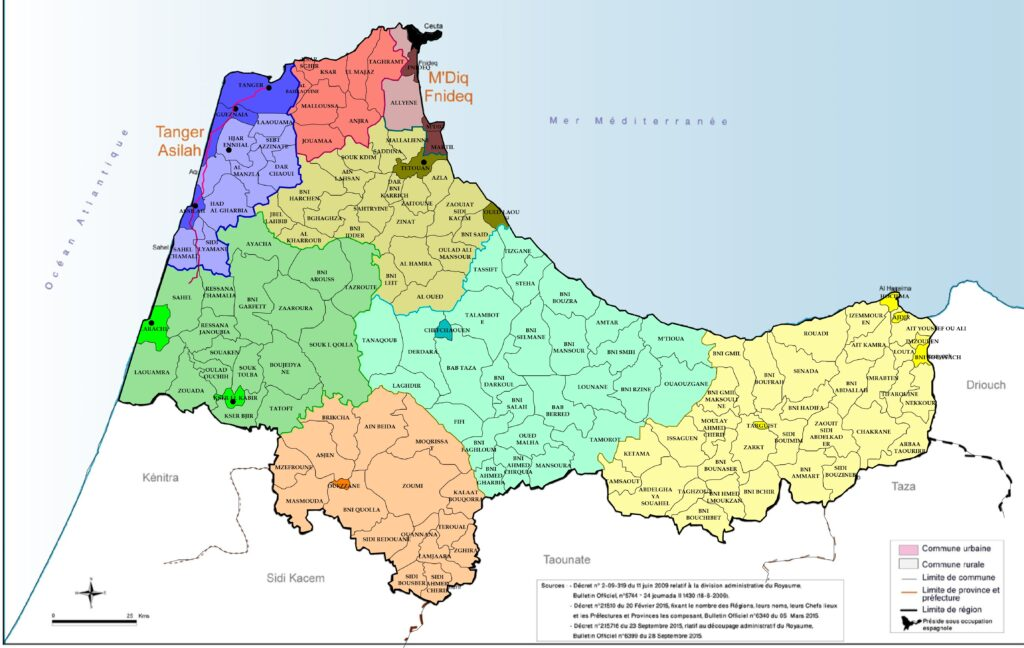
\includegraphics[width=\textwidth]{images/tanger-tetouan-al-houceima-region-map.jpeg}
    \caption{Carte de la région Tanger--Tétouan--Al Hoceïma}
    \label{fig:map-region}
\end{subfigure}
\caption{Présentation du Groupement Sanitaire Territorial Tanger--Tétouan--Al Hoceïma}
\label{fig:gst_presentation}
\end{figure}

%%%%%%%%%%%%%%%%%%%%%%%%%%%%%%%%%%%%%%%%%%%%%%%%%%%%%%%%%%%%%%%%%%%%%%%%%%%%%%
\subsection{Fiche signalétique}

Les principales informations relatives à l'organisme d'accueil sont présentées dans le tableau~\ref{tab:gst}.

\begin{table}[H]
\centering
\rowcolors{2}{LightGray}{white}
\begin{tabularx}{\textwidth}{>{\bfseries}p{4cm}X}
\toprule
\rowcolor{TableHeader}
\color{white}Élément & \color{white}Description \\
\midrule
Raison sociale & Groupement Sanitaire Territorial Tanger--Tétouan--Al Hoceïma (GST-TTA) \\
Tutelle & Ministère de la Santé et de la Protection Sociale \\
Statut juridique & Établissement public de santé, sous la tutelle de l'État \\
Région couverte & Tanger--Tétouan--Al Hoceïma \\
Population desservie & Environ 3,7 millions d'habitants \\
Siège & Tanger \\
Site web & \url{https://gst-tta.ma} \\
Direction d'accueil & Direction de la Formation, de la Recherche et de l'Innovation \\
\bottomrule
\end{tabularx}
\caption{Fiche signalétique du GST-TTA}
\label{tab:gst}
\end{table}

%%%%%%%%%%%%%%%%%%%%%%%%%%%%%%%%%%%%%%%%%%%%%%%%%%%%%%%%%%%%%%%%%%%%%%%%%%%%%%
\subsection{Missions}

Le GST-TTA assure la gouvernance des établissements de santé de la région et veille à l'amélioration continue de la qualité des services proposés aux citoyens.

Ses principales missions sont les suivantes :

\begin{itemize}
  \item coordonner les établissements hospitaliers de la région ;
  \item améliorer la qualité, la sécurité et la continuité des soins ;
  \item optimiser la gestion des ressources humaines, matérielles et financières ;
  \item accompagner la transformation numérique du système hospitalier ;
  \item promouvoir la recherche scientifique et l'innovation médicale ;
  \item développer les programmes de formation destinés aux professionnels de santé.
\end{itemize}

L'ensemble de ces missions contribue à renforcer l'efficacité du système de santé régional tout en favorisant l'introduction de solutions numériques innovantes. Ces missions, notamment l'accompagnement de la transformation numérique et la promotion de l'innovation, justifient le développement d'une plateforme comme celle présentée dans ce mémoire.

%%%%%%%%%%%%%%%%%%%%%%%%%%%%%%%%%%%%%%%%%%%%%%%%%%%%%%%%%%%%%%%%%%%%%%%%%%%%%%
\subsection{Organisation}

Le Groupement Sanitaire Territorial est organisé autour d'une direction générale appuyée par plusieurs directions fonctionnelles couvrant les domaines médicaux, administratifs, financiers, techniques ainsi que les activités liées à la recherche et à l'innovation.

Cette organisation favorise une gouvernance intégrée des établissements de santé et facilite la conduite de projets transversaux, notamment ceux liés à la transformation numérique.

\begin{figure}[H]
\centering
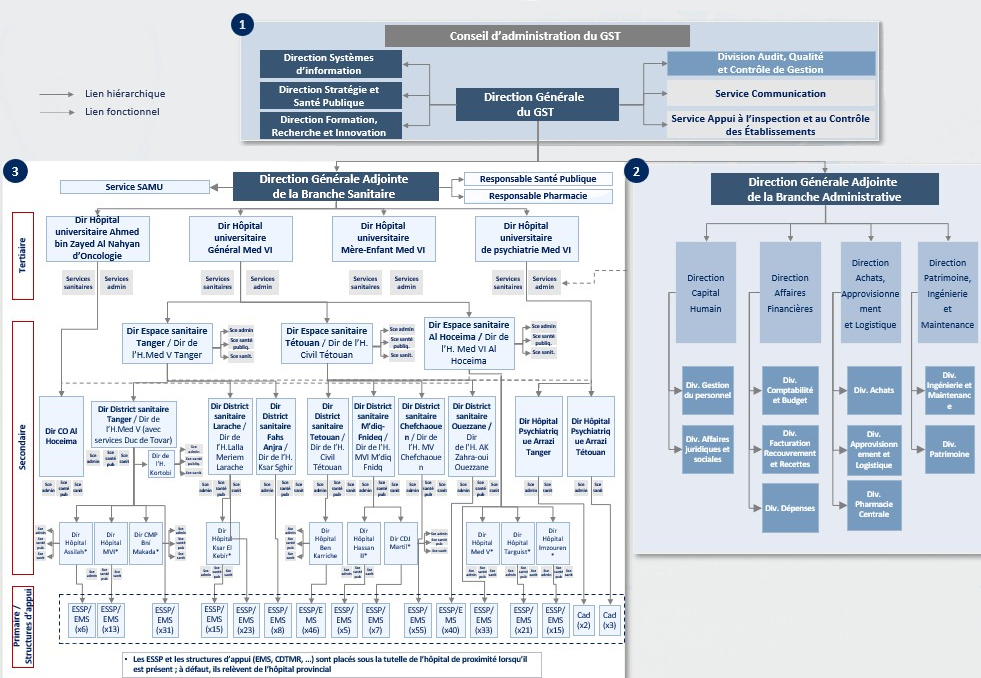
\includegraphics[width=0.92\textwidth]{images/3-Organigramme-general-GST-TTA.jpg}
\caption{Organigramme du Groupement Sanitaire Territorial Tanger--Tétouan--Al Hoceïma}
\label{fig:organigramme_gst}
\end{figure}

%%%%%%%%%%%%%%%%%%%%%%%%%%%%%%%%%%%%%%%%%%%%%%%%%%%%%%%%%%%%%%%%%%%%%%%%%%%%%%
\subsection{Direction de la Formation, de la Recherche et de l'Innovation}

Le projet a été réalisé au sein de la \textbf{Direction de la Formation, de la Recherche et de l'Innovation (DFRI)}.

Cette direction constitue un acteur majeur de la stratégie d'innovation du Groupement. Elle accompagne les établissements de santé dans leurs activités de formation, coordonne les projets de recherche et favorise le développement de solutions numériques répondant aux besoins du secteur hospitalier.

Parmi ses principales missions figurent :

\begin{itemize}
  \item la coordination des activités de formation ;
  \item le développement de projets de recherche scientifique ;
  \item la promotion de l'innovation technologique ;
  \item la valorisation des données de santé ;
  \item l'accompagnement des projets de transformation numérique.
\end{itemize}

Le développement de la plateforme présentée dans ce mémoire s'inscrit pleinement dans cette démarche de modernisation des outils d'aide à la décision fondés sur l'intelligence artificielle.

\begin{infobox}{Positionnement du projet}
Le projet a été réalisé au sein de la Direction de la Formation, de la Recherche et de l'Innovation du GST-TTA. Il contribue à la stratégie de transformation numérique de l'établissement en proposant une plateforme conversationnelle capable de faciliter l'exploitation des données grâce à l'intelligence artificielle générative.
\end{infobox}

%%%%%%%%%%%%%%%%%%%%%%%%%%%%%%%%%%%%%%%%%%%%%%%%%%%%%%%%%%%%%%%%%%%%%%%%%%%%%%
\section{Contexte général et analyse de l'existant}
%%%%%%%%%%%%%%%%%%%%%%%%%%%%%%%%%%%%%%%%%%%%%%%%%%%%%%%%%%%%%%%%%%%%%%%%%%%%%%

Le secteur de la santé connaît actuellement une profonde transformation numérique, marquée par la généralisation des systèmes d'information hospitaliers et la multiplication des données produites au quotidien. Cette évolution offre de nouvelles perspectives pour le pilotage des établissements de santé, l'amélioration de la qualité des soins et l'aide à la prise de décision.

Dans ce contexte, le Groupement Sanitaire Territorial Tanger--Tétouan--Al Hoceïma (GST-TTA) poursuit la modernisation de son infrastructure numérique afin de renforcer la gestion des établissements hospitaliers de la région. Toutefois, malgré la disponibilité d'un volume considérable de données, leur exploitation demeure complexe en raison des outils utilisés, de la diversité des sources d'information et des contraintes propres au domaine de la santé.

Cette section présente le contexte numérique du GST-TTA, les caractéristiques des données manipulées, le processus actuel d'analyse ainsi que les principales limites des solutions existantes.

%%%%%%%%%%%%%%%%%%%%%%%%%%%%%%%%%%%%%%%%%%%%%%%%%%%%%%%%%%%%%%%%%%%%%%%%%%%%%%
\subsection{Transformation numérique au GST-TTA}
%%%%%%%%%%%%%%%%%%%%%%%%%%%%%%%%%%%%%%%%%%%%%%%%%%%%%%%%%%%%%%%%%%%%%%%%%%%%%%

Dans le cadre de la réforme du système national de santé, le GST-TTA s'inscrit dans une stratégie visant à accélérer la transformation numérique des établissements hospitaliers de la région. Cette stratégie repose sur la modernisation des processus administratifs, le développement des systèmes d'information hospitaliers ainsi que l'amélioration de la gouvernance fondée sur les données.

La digitalisation progressive des activités permet aujourd'hui de dématérialiser de nombreux processus auparavant réalisés de manière manuelle, tout en facilitant la circulation de l'information entre les différents établissements du groupement.

Parmi les principaux axes de cette transformation figurent notamment :

\begin{itemize}
  \item la numérisation des processus administratifs et médicaux ;
  \item l'amélioration de la qualité et de la disponibilité des données ;
  \item le développement d'outils décisionnels ;
  \item la promotion des projets d'innovation numérique ;
  \item l'intégration progressive des technologies d'intelligence artificielle.
\end{itemize}

Cette évolution permet au GST-TTA de disposer d'un environnement numérique de plus en plus riche, capable de soutenir efficacement les activités de pilotage et d'aide à la décision.

%%%%%%%%%%%%%%%%%%%%%%%%%%%%%%%%%%%%%%%%%%%%%%%%%%%%%%%%%%%%%%%%%%%%%%%%%%%%%%
\subsection{Données et systèmes d'information hospitaliers}
%%%%%%%%%%%%%%%%%%%%%%%%%%%%%%%%%%%%%%%%%%%%%%%%%%%%%%%%%%%%%%%%%%%%%%%%%%%%%%

Les établissements hospitaliers produisent quotidiennement un volume important de données provenant de multiples systèmes d'information. Ces données concernent aussi bien les activités médicales que les aspects administratifs, logistiques et financiers.

Parmi les principales catégories de données exploitées, on distingue :

\begin{itemize}
  \item les données relatives aux patients et aux hospitalisations ;
  \item les consultations et actes médicaux ;
  \item les résultats des laboratoires ;
  \item les données de pharmacie ;
  \item les ressources humaines ;
  \item les indicateurs de performance hospitalière ;
  \item les données financières et logistiques.
\end{itemize}

Ces informations présentent plusieurs caractéristiques qui rendent leur exploitation particulièrement complexe :

\begin{itemize}
  \item un volume très important de données ;
  \item une mise à jour continue des informations ;
  \item une diversité des formats et des sources ;
  \item un niveau élevé de sensibilité nécessitant des mesures strictes de confidentialité ;
  \item des besoins croissants en matière d'analyse et de visualisation.
\end{itemize}

L'ensemble de ces données constitue une ressource stratégique permettant d'améliorer le suivi des activités hospitalières et de soutenir les décisions des responsables médicaux et administratifs.

%%%%%%%%%%%%%%%%%%%%%%%%%%%%%%%%%%%%%%%%%%%%%%%%%%%%%%%%%%%%%%%%%%%%%%%%%%%%%%
\subsection{Processus actuel et difficultés rencontrées}
%%%%%%%%%%%%%%%%%%%%%%%%%%%%%%%%%%%%%%%%%%%%%%%%%%%%%%%%%%%%%%%%%%%%%%%%%%%%%%

À l'heure actuelle, l'exploitation des données repose principalement sur une succession d'étapes réalisées à l'aide de plusieurs outils distincts.

Le processus classique comprend généralement :

\begin{enumerate}
  \item l'extraction des données depuis les différents systèmes d'information ;
  \item le nettoyage et la préparation des jeux de données ;
  \item la réalisation des traitements statistiques ;
  \item la création des tableaux et graphiques ;
  \item l'interprétation des résultats ;
  \item la rédaction des rapports.
\end{enumerate}

Bien que cette approche permette d'obtenir les analyses souhaitées, elle présente plusieurs inconvénients majeurs.

Les utilisateurs doivent souvent maîtriser plusieurs logiciels spécialisés tels que Microsoft Excel, SQL, Python ou encore Power BI. Cette multiplicité d'outils implique des manipulations répétitives, augmente les risques d'erreurs et allonge considérablement le temps nécessaire à la production des résultats.

Par ailleurs, la majorité des professionnels de santé ne disposent pas nécessairement des compétences techniques requises pour réaliser des analyses complexes, ce qui limite leur autonomie dans l'exploitation des données et crée une dépendance vis-à-vis des services spécialisés.

%%%%%%%%%%%%%%%%%%%%%%%%%%%%%%%%%%%%%%%%%%%%%%%%%%%%%%%%%%%%%%%%%%%%%%%%%%%%%%
\subsection{Limites des solutions existantes}
%%%%%%%%%%%%%%%%%%%%%%%%%%%%%%%%%%%%%%%%%%%%%%%%%%%%%%%%%%%%%%%%%%%%%%%%%%%%%%

Les solutions actuellement disponibles présentent trois limites majeures qui freinent l'exploitation efficace des données de santé.

\subsubsection*{Barrière technique}

Les outils traditionnels d'analyse de données (Excel, SQL, Power BI, Python) exigent des compétences techniques avancées en programmation, en statistiques ou en gestion de bases de données. Leur utilisation reste donc largement réservée aux profils spécialisés, limitant ainsi l'accès à l'information pour les utilisateurs métiers (médecins, personnels administratifs, décideurs).

\subsubsection*{Problèmes de confidentialité}

L'émergence des assistants conversationnels basés sur les grands modèles de langage (LLMs), tels que ChatGPT, Claude ou Gemini, a ouvert de nouvelles perspectives pour l'analyse de données en langage naturel. Ces interfaces réduisent considérablement la barrière technique et permettent à des utilisateurs non spécialistes d'interroger leurs données.

Toutefois, ces plateformes publiques ne répondent pas aux exigences de confidentialité imposées par le secteur de la santé. Les données médicales réelles, contenant des informations sensibles relatives aux patients, sont soumises à des contraintes réglementaires et éthiques strictes. Leur transmission vers des services externes hébergés sur des infrastructures publiques représente un risque majeur pour la sécurité, la confidentialité et la souveraineté des données.

\subsubsection*{Fragmentation des outils}

Les utilisateurs sont souvent contraints de manipuler plusieurs outils distincts afin de préparer les données, réaliser les analyses statistiques, produire des visualisations puis rédiger des rapports. Cette fragmentation du processus complexifie le travail, augmente le risque d'erreurs et ralentit considérablement la prise de décision.

De plus, les assistants conversationnels existants reposent principalement sur des mécanismes de génération de texte. Ils ne garantissent pas toujours la reproductibilité des traitements analytiques, la traçabilité des calculs effectués ni la transparence des résultats obtenus.

\begin{infobox}{Synthèse de l'analyse}
L'analyse de l'existant montre que les établissements de santé disposent aujourd'hui d'un patrimoine informationnel considérable, mais que son exploitation demeure freinée par trois obstacles majeurs : (i) la complexité technique des outils, (ii) les contraintes de confidentialité des données de santé, et (iii) la fragmentation des processus d'analyse.

Ces limites mettent en évidence la nécessité de disposer d'une plateforme intégrée, capable de combiner les avantages des interfaces conversationnelles avec la fiabilité d'un moteur d'analyse déterministe, tout en assurant la confidentialité des données manipulées.
\end{infobox}

%%%%%%%%%%%%%%%%%%%%%%%%%%%%%%%%%%%%%%%%%%%%%%%%%%%%%%%%%%%%%%%%%%%%%%%%%%%%%%
\section{Problématique}
%%%%%%%%%%%%%%%%%%%%%%%%%%%%%%%%%%%%%%%%%%%%%%%%%%%%%%%%%%%%%%%%%%%%%%%%%%%%%%

L'exploitation des données constitue aujourd'hui un enjeu majeur pour les établissements de santé. Avec la généralisation des systèmes d'information hospitaliers, les établissements produisent quotidiennement un volume considérable de données issues de multiples sources : dossiers médicaux électroniques, systèmes d'information hospitaliers, laboratoires, services administratifs, indicateurs de performance et données de recherche.

Ces données sont non seulement \textbf{massives}, mais également \textbf{dynamiques}, puisqu'elles sont continuellement mises à jour pour refléter l'évolution des activités médicales et administratives.

Les constats établis dans l'analyse de l'existant — barrière technique, problèmes de confidentialité et fragmentation des outils — mettent en évidence la nécessité de disposer d'une solution capable d'exploiter efficacement des données sensibles tout en restant simple d'utilisation, sécurisée et adaptée aux besoins des établissements de santé.

Ainsi, la problématique centrale de ce projet peut être formulée comme suit :

\begin{quote}
\itshape
\small
\textbf{\hl{Comment concevoir une plateforme intelligente permettant aux professionnels de santé d'interagir avec des jeux de données massifs et continuellement mis à jour en langage naturel, tout en garantissant la confidentialité des données sensibles, la fiabilité des traitements analytiques, la transparence des résultats, la modularité du système et la reproductibilité des analyses ?}}
\end{quote}

Cette problématique soulève plusieurs défis complémentaires :

\begin{itemize}
  \item \textbf{Défi technique} : concevoir une architecture modulaire séparant l'orchestration pilotée par l'IA de l'exécution computationnelle déterministe ;
  \item \textbf{Défi sécuritaire} : garantir la confidentialité et la souveraineté des données de santé tout en offrant des fonctionnalités d'analyse avancées ;
  \item \textbf{Défi d'usage} : proposer une interface intuitive permettant à des utilisateurs non techniques d'exploiter efficacement leurs données ;
  \item \textbf{Défi d'extensibilité} : développer une solution facilement adaptable à l'évolution des besoins et des technologies.
\end{itemize}

%%%%%%%%%%%%%%%%%%%%%%%%%%%%%%%%%%%%%%%%%%%%%%%%%%%%%%%%%%%%%%%%%%%%%%%%%%%%%%
\section{Objectifs du projet}
%%%%%%%%%%%%%%%%%%%%%%%%%%%%%%%%%%%%%%%%%%%%%%%%%%%%%%%%%%%%%%%%%%%%%%%%%%%%%%

\subsection{Objectif général}

L'objectif général de ce projet consiste à \textbf{concevoir et développer une plateforme conversationnelle d'analyse de données} reposant sur une architecture modulaire intégrant des agents d'intelligence artificielle. Cette plateforme doit permettre aux utilisateurs d'exploiter efficacement leurs données sans nécessiter de compétences avancées en programmation ou en science des données.

\subsection{Objectifs spécifiques}

Afin d'atteindre cet objectif général, plusieurs objectifs spécifiques ont été définis :

\begin{enumerate}
  \item \textbf{Conception architecturale} : concevoir une architecture logicielle modulaire favorisant la maintenabilité et l'évolutivité de la plateforme ;
  
  \item \textbf{Interface conversationnelle} : développer une interface conversationnelle intuitive permettant d'interroger les données en langage naturel ;
  
  \item \textbf{Orchestration intelligente} : intégrer un agent intelligent capable d'orchestrer les différentes étapes d'une analyse de données ;
  
  \item \textbf{Automatisation des traitements} : automatiser les traitements statistiques ainsi que les opérations courantes de préparation et d'exploration des données ;
  
  \item \textbf{Visualisation automatique} : générer automatiquement des visualisations adaptées aux résultats obtenus ;
  
  \item \textbf{Persistance des données} : permettre la gestion et la persistance des conversations ainsi que des artefacts produits au cours des analyses ;
  
  \item \textbf{Communication fluide} : assurer une communication fluide entre les différents composants de la plateforme grâce à une architecture moderne basée sur des API REST et le streaming des réponses ;
  
  \item \textbf{Extensibilité} : développer une solution facilement extensible permettant l'ajout de nouveaux outils d'analyse et de nouveaux modèles d'intelligence artificielle.
\end{enumerate}

%%%%%%%%%%%%%%%%%%%%%%%%%%%%%%%%%%%%%%%%%%%%%%%%%%%%%%%%%%%%%%%%%%%%%%%%%%%%%%
\section{Méthodologie adoptée}
%%%%%%%%%%%%%%%%%%%%%%%%%%%%%%%%%%%%%%%%%%%%%%%%%%%%%%%%%%%%%%%%%%%%%%%%%%%%%%

La réalisation de ce projet s'est appuyée sur une démarche de développement agile, adaptée aux spécificités d'un projet de recherche et développement en intelligence artificielle. Cette approche itérative et incrémentale a permis une progression maîtrisée, depuis une vision large de la plateforme jusqu'à une spécialisation progressive dans le domaine de la santé, en intégrant les retours des parties prenantes à chaque étape.

\begin{figure}[H]
\centering
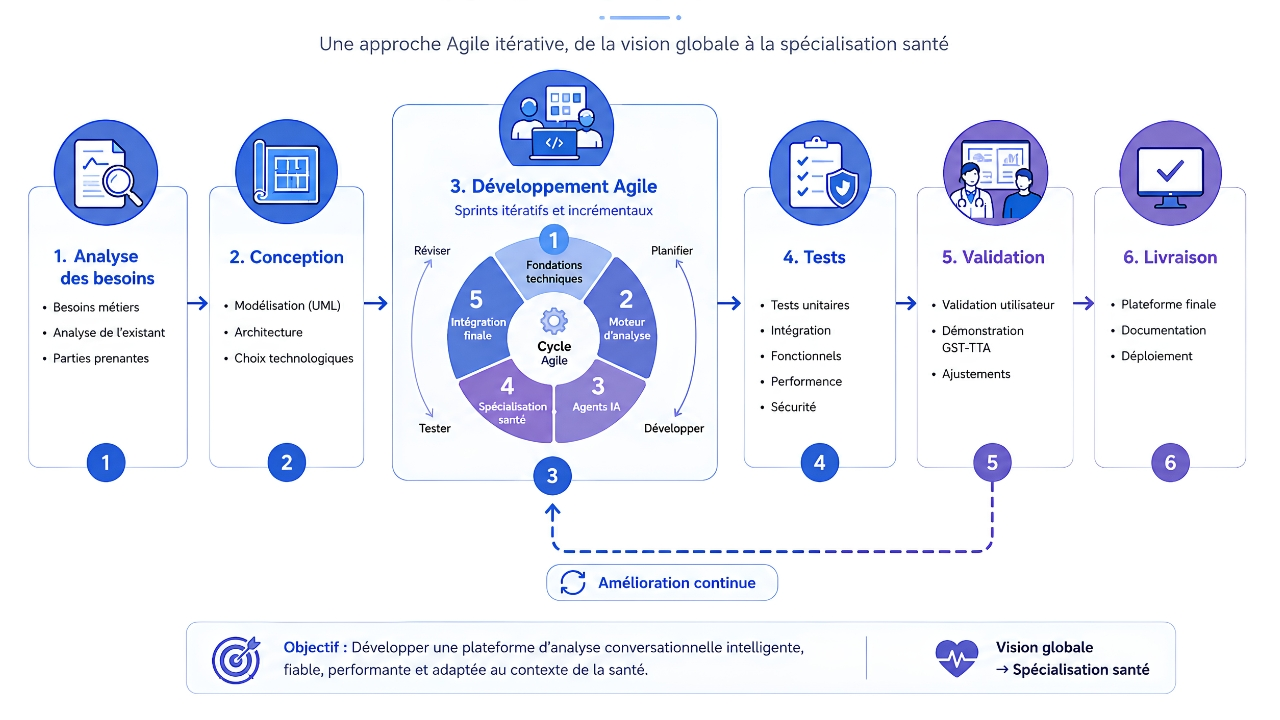
\includegraphics[width=0.82\textwidth]{images/methodologie.jpg}
\caption{Démarche générale adoptée pour la réalisation du projet}
\label{fig:methodologie}
\end{figure}

\subsection{Approche Agile adaptée}

Notre méthodologie s'inscrit dans une logique Agile, caractérisée par des cycles de développement courts (sprints) et une livraison incrémentale des fonctionnalités. Cette approche a été particulièrement adaptée à notre contexte, où les besoins ont évolué d'une vision générique vers une spécialisation progressive.

\begin{figure}[H]
\centering
\begin{tikzpicture}[
    node distance=0.8cm,
    phase/.style={rectangle, draw, thick, minimum width=5cm, minimum height=0.6cm, align=center, rounded corners, fill=LightGray!50},
    arrow/.style={->, thick, color=PrimaryRed, -{Stealth[length=3mm]}}
]
\node[phase, fill=PrimaryRed!15] (vision) {Vision globale de la plateforme};
\node[phase, below=of vision] (sprint1) {Sprint 1 : Fondations techniques};
\node[phase, below=of sprint1] (sprint2) {Sprint 2 : Moteur d'analyse};
\node[phase, below=of sprint2] (sprint3) {Sprint 3 : Agents IA};
\node[phase, below=of sprint3] (sprint4) {Sprint 4 : Spécialisation santé};
\node[phase, below=of sprint4, fill=PrimaryRed!25] (sprint5) {Sprint 5 : Intégration \& finalisation};

\draw[arrow] (vision) -- (sprint1);
\draw[arrow] (sprint1) -- (sprint2);
\draw[arrow] (sprint2) -- (sprint3);
\draw[arrow] (sprint3) -- (sprint4);
\draw[arrow] (sprint4) -- (sprint5);

% Feedback arrows
\draw[->, color=PrimaryRed, dashed, thick] (sprint2.west) -- ++(-1.2,0) |- (sprint1.west)
    node[pos=0.15, left, font=\scriptsize\itshape] {Retours};
\draw[->, color=PrimaryRed, dashed, thick] (sprint3.west) -- ++(-1.2,0) |- (sprint2.west);
\draw[->, color=PrimaryRed, dashed, thick] (sprint4.west) -- ++(-1.2,0) |- (sprint3.west);

% Annotation
\node[font=\small\itshape, color=MidGray, right=0.3cm of sprint3, xshift=2.5cm] {Spécialisation};
\node[font=\small\itshape, color=MidGray, right=0.3cm of sprint5, xshift=2.5cm] {Livraison};
\end{tikzpicture}
\caption{Structure des sprints : de la vision globale à la spécialisation santé}
\label{fig:sprints}
\end{figure}

\subsection{Organisation en sprints}

Le projet a été structuré en cinq sprints de deux à trois semaines, chacun ayant un objectif spécifique et livrant un incrément fonctionnel de la plateforme :

\begin{enumerate}
  \item \textbf{Sprint 1 : Fondations techniques} — Mise en place de l'infrastructure de base : structure du monorepo, environnement de développement, configuration des outils, et premier prototype d'interface.
  
  \item \textbf{Sprint 2 : Moteur d'analyse} — Développement du moteur computationnel (pandas, matplotlib) avec support multi-formats et fonctions statistiques essentielles.
  
  \item \textbf{Sprint 3 : Agents IA et orchestration} — Implémentation du framework agent (LangGraph), création des outils d'analyse, et mise en place de l'orchestrateur en trois phases.
  
  \item \textbf{Sprint 4 : Spécialisation santé} — Adaptation de la plateforme aux données du GST-TTA : intégration de jeux de données réels, personnalisation des analyses pour le contexte médical, et mise en place de la persistance.
  
  \item \textbf{Sprint 5 : Intégration et finalisation} — Assemblage complet des composants, tests d'intégration, optimisation des performances, et préparation de la livraison.
\end{enumerate}

Cette organisation a permis de maintenir un rythme de développement soutenu tout en assurant une validation continue des fonctionnalités produites.

\subsection{Phases de réalisation}

Au-delà de l'organisation en sprints, la réalisation du projet s'est articulée autour de quatre grandes phases complémentaires, permettant de structurer progressivement le développement de la plateforme.

\subsubsection{Phase 1 : Analyse des besoins}

Cette première phase a consisté à identifier les besoins des utilisateurs, à étudier le contexte du projet et à analyser les solutions existantes. Elle a permis de définir les objectifs du système ainsi que les principales exigences fonctionnelles et non fonctionnelles.

\subsubsection{Phase 2 : Conception et architecture}

La seconde phase a été consacrée à la modélisation de la solution et à la définition de son architecture logicielle. Les différents composants du système ont été conçus selon une approche modulaire afin de garantir leur maintenabilité, leur évolutivité et leur réutilisabilité.

\subsubsection{Phase 3 : Développement}

La troisième phase correspond à l'implémentation progressive de la plateforme selon une approche Agile. Les fonctionnalités ont été développées de manière incrémentale au cours de plusieurs sprints, permettant une validation continue des résultats obtenus et une adaptation aux besoins identifiés.

\subsubsection{Phase 4 : Tests et validation}

Enfin, une phase de validation a été menée afin de vérifier le bon fonctionnement de la plateforme. Différents niveaux de tests ont été réalisés pour évaluer la qualité de la solution, sa robustesse, ses performances ainsi que son adéquation aux objectifs fixés.

\begin{resultbox}{Synthèse méthodologique}
La méthodologie adoptée combine une approche Agile basée sur des développements itératifs avec une progression structurée en quatre phases : analyse, conception, développement et validation. Cette organisation a permis de faire évoluer progressivement la plateforme, depuis une vision générale jusqu'à une solution adaptée aux besoins du GST-TTA.
\end{resultbox}

%%%%%%%%%%%%%%%%%%%%%%%%%%%%%%%%%%%%%%%%%%%%%%%%%%%%%%%%%%%%%%%%%%%%%%%%%%%%%%
\section{Management du projet}
%%%%%%%%%%%%%%%%%%%%%%%%%%%%%%%%%%%%%%%%%%%%%%%%%%%%%%%%%%%%%%%%%%%%%%%%%%%%%%

La bonne conduite d'un projet de cette envergure nécessite une organisation rigoureuse, une répartition claire des responsabilités et un suivi temporel des différentes tâches. Cette section présente les principaux aspects du management du projet : l'équipe impliquée, la répartition des tâches et la planification temporelle.

\subsection{Équipe du projet}

Le projet a été mené par une équipe pluridisciplinaire, encadrée par des professionnels du GST-TTA et de l'établissement d'enseignement supérieur. L'équipe se compose comme suit :
\begin{table}[H]
\centering
\small
\renewcommand{\arraystretch}{1.25}

\begin{tabularx}{\textwidth}{
    >{\bfseries\raggedright\arraybackslash}p{3.3cm}
    >{\raggedright\arraybackslash}p{4.0cm}
    >{\raggedright\arraybackslash}X
}
\toprule
\rowcolor{TableHeader}
\color{white}\textbf{Rôle} &
\color{white}\textbf{Nom} &
\color{white}\textbf{Responsabilités} \\
\midrule

Stagiaires
&
El Gharib Mahmoud\par\medskip
Zarqi  Ezzoubair\par\medskip
El Attar Mohamed
&
\begin{itemize}[leftmargin=*,nosep]
    \item Analyse des structures et des sources de données ;
    \item Analyse et conception fonctionnelle et technique ;
    \item Modélisation et conception de l'architecture du système ;
    \item Développement de la plateforme et de ses différentes fonctionnalités ;
    \item Mise en place du moteur d'analyse et de l'orchestration agentique ;
    \item Intégration des modèles de langage et des composants d'intelligence artificielle ;
    \item Mise en place de la persistance, du cache et de la gestion des artefacts ;
    \item Réalisation des tests et validation des fonctionnalités ;
    \item Suivi des performances et amélioration de la solution ;
    \item Documentation et préparation de la soutenance.
\end{itemize}
\\

\midrule

Encadrante pédagogique
&
Pr.~Benabdoulah Ikram
&
Suivi académique du projet, orientation méthodologique,
correction et suivi du mémoire ainsi que préparation de la soutenance.
\\

\midrule

Encadrant technique
&
FANGACHI Oussama
&
Orientation technique, validation des fonctionnalités,
accompagnement du développement et exécution des tests.
\\

\bottomrule
\end{tabularx}

\caption{Composition de l'équipe projet et répartition des responsabilités}
\label{tab:equipe}
\end{table}
% \subsection{Répartition des tâches}

% La répartition des tâches a été organisée en fonction des compétences de chaque membre de l'équipe et des exigences du projet. Le tableau ci-dessous présente la répartition des principales activités :

% \begin{table}[H]
% \centering
% \caption{Répartition des tâches}
% \label{tab:repartition}
% \small
% \begin{tabularx}{\textwidth}{Y Z Z Z}
% \toprule
% \textbf{Tâche} & \textbf{Étudiant} & \textbf{Encadrant académique} & \textbf{Encadrant professionnel} \\
% \midrule
% Analyse des besoins & \textbullet & $\circ$ & \textbullet \\
% Conception architecturale & \textbullet & \textbullet & $\circ$ \\
% Développement backend & \textbullet & $\circ$ & $\circ$ \\
% Développement frontend & \textbullet & $\circ$ & $\circ$ \\
% Intégration des agents IA & \textbullet & $\circ$ & \textbullet \\
% Tests et validation & \textbullet & \textbullet & $\circ$ \\
% Rédaction du mémoire & \textbullet & \textbullet & $\circ$ \\
% \bottomrule
% \end{tabularx}
% \caption*{Légende : \textbullet\ Principal responsable, $\circ$ Contribution partielle}
% \end{table}

\subsection{Diagramme de Gantt}

La planification temporelle du projet a été établie sous forme de diagramme de Gantt, permettant de visualiser la séquence et la durée des différentes tâches. Ce diagramme couvre l'ensemble de la période de réalisation du projet, depuis l'analyse des besoins jusqu'à la livraison finale.

\begin{figure}[H]
\centering
\includegraphicsorplaceholder[width=0.95\textwidth]{gantt_projet_style_professionnel.png}
\caption{Diagramme de Gantt du projet}
\label{fig:gantt}
\end{figure}
La planification suit une organisation itérative dans laquelle plusieurs activités
peuvent être menées en parallèle. Cette organisation permet notamment
d'articuler progressivement la conception, le développement du moteur
d'analyse, l'intégration des agents d'intelligence artificielle,
l'implémentation du mécanisme de gestion du contexte, puis les phases
d'intégration, de validation et de documentation
\begin{resultbox}{Synthèse du management}
L'organisation du projet, structurée autour d'une équipe aux rôles clairement définis et d'une planification rigoureuse, a permis de mener à bien les différentes phases dans le respect des délais impartis. La répartition des tâches a favorisé une collaboration efficace entre les acteurs académiques et professionnels.
\end{resultbox}

%%%%%%%%%%%%%%%%%%%%%%%%%%%%%%%%%%%%%%%%%%%%%%%%%%%%%%%%%%%%%%%%%%%%%%%%%%%%%%
\section{Conclusion}
%%%%%%%%%%%%%%%%%%%%%%%%%%%%%%%%%%%%%%%%%%%%%%%%%%%%%%%%%%%%%%%%%%%%%%%%%%%%%%

Le Groupement Sanitaire Territorial Tanger--Tétouan--Al Hoceïma constitue un environnement particulièrement favorable au développement de projets innovants destinés à améliorer l'exploitation des données de santé. Grâce à sa stratégie de transformation numérique et à l'implication de la Direction de la Formation, de la Recherche et de l'Innovation, il offre un cadre propice à la conception de solutions d'aide à la décision intégrant les technologies de l'intelligence artificielle.

L'analyse du contexte et de l'existant a mis en évidence les limites des solutions actuelles, justifiant la nécessité de développer une plateforme adaptée aux besoins du secteur hospitalier. La problématique, les objectifs et la méthodologie adoptée constituent les fondements de la démarche entreprise.

L'organisation du projet, structurée autour d'une équipe pluridisciplinaire, d'une répartition claire des tâches et d'une planification temporelle rigoureuse, a permis d'assurer une conduite maîtrisée du projet dans le respect des échéances fixées.

Le chapitre suivant sera consacré à l'état de l'art des technologies et solutions existantes dans le domaine de l'analyse de données conversationnelle, des grands modèles de langage et des architectures d'agents intelligents qui constituent les fondements scientifiques de la plateforme développée.

%%%%%%%%%%%%%%%%%%%%%%%%%%%%%%%%%%%%%%%%%%%%%%%%%%%%%%%%%%%%%%%%%%%%%%%%%%%%%%
\chapter{Analyse des besoins et étude de l'existant}
%%%%%%%%%%%%%%%%%%%%%%%%%%%%%%%%%%%%%%%%%%%%%%%%%%%%%%%%%%%%%%%%%%%%%%%%%%%%%%

\section{Introduction}

Ce chapitre a pour objectif d'analyser les besoins auxquels doit répondre la plateforme proposée et d'étudier les solutions existantes dans le domaine de l'analyse conversationnelle de données. Dans un premier temps, les différents acteurs ainsi que leurs besoins fonctionnels et non fonctionnels sont identifiés afin de définir le périmètre du projet. Dans un second temps, un état de l'art présente les principales technologies mobilisées ainsi qu'une étude comparative des plateformes existantes. Cette analyse permet enfin de justifier les choix retenus pour la conception de la solution proposée.

%%%%%%%%%%%%%%%%%%%%%%%%%%%%%%%%%%%%%%%%%%%%%%%%%%%%%%%%%%%%%%%%%%%%%%%%%%%%%%
\section{Analyse des besoins}
%%%%%%%%%%%%%%%%%%%%%%%%%%%%%%%%%%%%%%%%%%%%%%%%%%%%%%%%%%%%%%%%%%%%%%%%%%%%%%

Cette section présente les besoins identifiés auprès des futurs utilisateurs de la plateforme. L'objectif est de définir les fonctionnalités attendues ainsi que les contraintes auxquelles le système devra répondre.

\subsection{Identification des acteurs}

L'identification des acteurs constitue une étape préliminaire essentielle pour comprendre les interactions entre les utilisateurs et le système. La plateforme s'adresse à plusieurs catégories d'utilisateurs ayant des rôles et des attentes distincts.

\begin{figure}[H]
\centering
\begin{tikzpicture}[
    actor/.style={rectangle, draw, thick, minimum width=3.5cm, minimum height=1cm, align=center, rounded corners, fill=PrimaryRed!10},
    system/.style={rectangle, draw, thick, minimum width=5cm, minimum height=0.8cm, align=center, rounded corners, fill=PrimaryRed!25, font=\bfseries},
    arrow/.style={->, thick, color=PrimaryRed, -{Stealth[length=3mm]}}
]
\node[system] (system) {Plateforme CHU};
\node[actor, above left=1cm and 1.5cm of system] (medecin) {Médecins \\ \small Professionnels de santé};
\node[actor, above=0.5cm of system] (administratif) {Personnels \\ \small Administratifs et décideurs};
\node[actor, above right=1cm and 1.5cm of system] (data) {Data Scientists \\ \small Analystes et chercheurs};

\draw[arrow] (medecin) -- (system);
\draw[arrow] (administratif) -- (system);
\draw[arrow] (data) -- (system);
\end{tikzpicture}
\caption{Acteurs principaux de la plateforme}
\label{fig:acteurs}
\end{figure}

Les acteurs identifiés sont les suivants :

\begin{itemize}
  \item \textbf{Médecins et professionnels de santé} : utilisateurs finaux souhaitant interroger les données en langage naturel pour obtenir des analyses rapides sur leurs activités ;
  \item \textbf{Personnels administratifs et décideurs} : responsables du pilotage des établissements cherchant à suivre les indicateurs de performance et à prendre des décisions fondées sur les données ;
  \item \textbf{Data scientists et analystes} : utilisateurs techniques nécessitant des fonctionnalités avancées pour des analyses complexes et reproductibles.
\end{itemize}

\subsection{Cas d'utilisation}

Les cas d'utilisation principaux de la plateforme sont présentés dans le diagramme ci-dessous :

\begin{figure}[H]
\centering
\begin{tikzpicture}[
    usecase/.style={ellipse, draw, thick, minimum width=3cm, minimum height=1.2cm, align=center, fill=SoftRed!20},
    actor/.style={rectangle, draw, thick, minimum width=2.5cm, minimum height=0.8cm, align=center, rounded corners, fill=PrimaryRed!10},
    arrow/.style={->, thick, color=PrimaryRed, -{Stealth[length=3mm]}}
]
\node[actor] (user) {Utilisateur};
\node[usecase, above right=0.5cm and 1cm of user] (uc1) {Importer \\ des données};
\node[usecase, right=1.5cm of uc1] (uc2) {Interroger en \\ langage naturel};
\node[usecase, right=1.5cm of uc2] (uc3) {Visualiser \\ les résultats};
\node[usecase, below=0.5cm of uc1] (uc4) {Exporter \\ des rapports};
\node[usecase, below=0.5cm of uc2] (uc5) {Gérer ses \\ conversations};
\node[usecase, below=0.5cm of uc3] (uc6) {Partager \\ des analyses};

\draw[arrow] (user) -- (uc1);
\draw[arrow] (user) -- (uc2);
\draw[arrow] (user) -- (uc3);
\draw[arrow] (user) -- (uc4);
\draw[arrow] (user) -- (uc5);
\draw[arrow] (user) -- (uc6);
\end{tikzpicture}
\caption{Diagramme des cas d'utilisation principaux}
\label{fig:cas_utilisation}
\end{figure}

\subsection{Besoins fonctionnels}

Les besoins fonctionnels décrivent les fonctionnalités que la plateforme doit offrir aux utilisateurs :

\begin{itemize}
  \item \textbf{Importation de données} : support multi-formats (CSV, XLSX, parquet, JSON) avec détection automatique de l'encodage et du délimiteur ;
  \item \textbf{Interaction en langage naturel} : interface conversationnelle permettant de formuler des requêtes analytiques sans compétences techniques ;
  \item \textbf{Planification automatique} : décomposition automatique d'une requête complexe en une séquence d'étapes ordonnées et traçables ;
  \item \textbf{Analyse statistique} : calculs statistiques rigoureux (descriptives, corrélations, agrégations, profilage) via un moteur déterministe ;
  \item \textbf{Visualisation automatique} : génération automatique de graphiques adaptés (histogrammes, diagrammes de dispersion, matrices de corrélation) ;
  \item \textbf{Génération de rapports} : production de rapports synthétiques intégrant résultats, graphiques et interprétations ;
  \item \textbf{Streaming en temps réel} : diffusion progressive des résultats (plan, étapes, graphiques, tokens) pour une expérience interactive ;
  \item \textbf{Persistance} : sauvegarde des conversations et des artefacts (graphiques, rapports) entre les sessions ;
  \item \textbf{Gestion des erreurs} : messages d'erreur clairs et suggestions pour guider l'utilisateur.
\end{itemize}

\subsection{Besoins non fonctionnels}

Les besoins non fonctionnels définissent les qualités et contraintes du système :

\begin{itemize}
  \item \textbf{Sécurité} : confidentialité et intégrité des données sensibles, authentification des utilisateurs, chiffrement des communications ;
  \item \textbf{Performance} : réactivité optimale avec un temps de réponse inférieur à 5 secondes pour les opérations courantes ;
  \item \textbf{Modularité} : architecture permettant l'ajout de nouveaux outils, agents ou visualisations sans modifications majeures ;
  \item \textbf{Extensibilité} : intégration facilitée de nouveaux modèles de langage et de nouvelles sources de données ;
  \item \textbf{Traçabilité} : journalisation des actions et des résultats pour l'audit et la reproductibilité des analyses ;
  \item \textbf{Maintenabilité} : bonnes pratiques de développement (tests unitaires, documentation, intégration continue) ;
  \item \textbf{Portabilité} : déploiement sur différentes infrastructures via la conteneurisation (Docker) ;
  \item \textbf{Souveraineté des données} : hébergement exclusif sur l'infrastructure du GST-TTA, sans transmission vers des services externes.
\end{itemize}

\begin{infobox}{Synthèse des besoins}
L'analyse des besoins a permis d'identifier une plateforme intégrée, sécurisée et modulaire, capable de répondre aux exigences du contexte hospitalier tout en offrant une interface intuitive en langage naturel. Les besoins non fonctionnels, notamment la sécurité et la souveraineté des données, constituent des contraintes fortes qui orientent les choix architecturaux.
\end{infobox}

%%%%%%%%%%%%%%%%%%%%%%%%%%%%%%%%%%%%%%%%%%%%%%%%%%%%%%%%%%%%%%%%%%%%%%%%%%%%%%
\section{État de l'art}
%%%%%%%%%%%%%%%%%%%%%%%%%%%%%%%%%%%%%%%%%%%%%%%%%%%%%%%%%%%%%%%%%%%%%%%%%%%%%%

Afin de concevoir une solution adaptée aux besoins identifiés, il est nécessaire d'étudier les principales technologies utilisées dans le domaine de l'intelligence artificielle générative et de l'analyse conversationnelle de données.

\subsection{Intelligence artificielle générative}

L'intelligence artificielle générative désigne l'ensemble des modèles capables de produire du contenu original — textes, images, code, etc. — à partir d'une entrée donnée. Contrairement aux modèles discriminants qui classifient ou prédisent, les modèles génératifs apprennent la distribution sous-jacente des données pour en générer de nouvelles.

Les avancées récentes dans ce domaine, notamment avec l'architecture Transformers et le mécanisme d'attention, ont permis l'émergence de modèles de plus en plus performants, capables de comprendre et de générer un langage naturel de qualité.

\subsection{Grands modèles de langage (LLMs)}

Les grands modèles de langage (\textit{Large Language Models}) sont des modèles d'IA générative entraînés sur des corpus textuels massifs. Ils sont capables de comprendre des requêtes en langage naturel, de raisonner sur des informations complexes et de générer des réponses cohérentes.

Parmi les LLMs les plus connus, on peut citer :

\begin{itemize}
  \item \textbf{GPT (OpenAI)} : modèles généralistes aux capacités étendues ;
  \item \textbf{Claude (Anthropic)} : modèle axé sur la sécurité et la fiabilité ;
  \item \textbf{Gemini (Google)} : modèle multimodal intégrant texte et image ;
  \item \textbf{Llama (Meta)} : modèle open source permettant un déploiement local.
\end{itemize}

Les LLMs ouvrent la voie à de nouvelles interfaces conversationnelles où l'utilisateur interagit en langage naturel, sans nécessiter de compétences techniques particulières.

\subsection{Agents intelligents}

Un agent intelligent est un système capable de percevoir son environnement, de raisonner sur les actions à entreprendre et d'agir de manière autonome pour atteindre un objectif. Dans le contexte de l'analyse de données, un agent peut orchestrer différentes étapes du traitement, appeler des outils spécialisés et synthétiser les résultats.

Les frameworks d'agents permettent aujourd'hui de :

\begin{itemize}
  \item décomposer des tâches complexes en sous-objectifs ;
  \item sélectionner dynamiquement les outils adaptés ;
  \item maintenir un état de la conversation ;
  \item assurer la traçabilité des actions effectuées.
\end{itemize}

\subsection{Model Context Protocol (MCP)}

Le Model Context Protocol est un protocole standardisé permettant aux modèles de langage d'interagir avec des outils et des sources de données externes de manière structurée. Il définit des interfaces communes pour :

\begin{itemize}
  \item la découverte des outils disponibles ;
  \item l'invocation des outils avec des paramètres validés ;
  \item le retour des résultats dans un format exploitable.
\end{itemize}

Ce protocole facilite l'intégration de nouvelles capacités aux agents sans modifier leur logique centrale.

\subsection{Framework LangGraph}

LangGraph est un framework open source permettant de construire des applications d'agents avec des graphes d'états. Il étend les capacités de LangChain en offrant :

\begin{itemize}
  \item une modélisation explicite du flux de contrôle ;
  \item la persistance de l'état entre les étapes ;
  \item la gestion de cycles et de conditionnels ;
  \item une traçabilité complète des actions.
\end{itemize}

Cette approche est particulièrement adaptée aux workflows analytiques complexes où chaque étape doit être documentée et vérifiable.



\subsection{Retrieval-Augmented Generation (RAG)}

Le RAG est une approche combinant la génération de texte avec la recherche d'informations dans des bases de données. Elle permet aux LLMs de produire des réponses basées sur des documents spécifiques plutôt que sur leur seule connaissance interne.

Les bénéfices du RAG incluent :

\begin{itemize}
  \item une réduction des hallucinations du modèle ;
  \item la capacité à répondre sur des données spécifiques non incluses dans l'entraînement ;
  \item la traçabilité des sources d'information.
\end{itemize}

Dans le contexte de l'analyse de données, le RAG peut être utilisé pour fournir des informations contextuelles sur les données (métadonnées, schémas, descriptions) lors de l'interprétation des résultats.

\subsection{Analyse conversationnelle de données}

L'analyse conversationnelle de données est un domaine émergent qui combine interfaces en langage naturel, intelligence artificielle et visualisation de données. Elle permet aux utilisateurs de dialoguer avec leurs données sans avoir à maîtriser des langages de programmation ou des outils statistiques complexes.

Les systèmes d'analyse conversationnelle reposent généralement sur :

\begin{itemize}
  \item une compréhension du langage naturel pour interpréter les requêtes ;
  \item un moteur d'exécution pour réaliser les traitements demandés ;
  \item une génération de langage naturel pour expliquer les résultats ;
  \item une interface de visualisation interactive.
\end{itemize}

%%%%%%%%%%%%%%%%%%%%%%%%%%%%%%%%%%%%%%%%%%%%%%%%%%%%%%%%%%%%%%%%%%%%%%%%%%%%%%
\section{Étude comparative des solutions existantes}
%%%%%%%%%%%%%%%%%%%%%%%%%%%%%%%%%%%%%%%%%%%%%%%%%%%%%%%%%%%%%%%%%%%%%%%%%%%%%%

Cette section présente une comparaison des principales plateformes actuellement disponibles pour l'analyse conversationnelle de données.

\begin{table}[H]
\centering
\caption{Comparaison des principales plateformes d'analyse conversationnelle}
\label{tab:comparaison}
\rowcolors{2}{LightGray}{white}
\begin{tabularx}{\textwidth}{>{\bfseries}p{3.3cm}cccccc}
\toprule
\rowcolor{TableHeader}
\color{white}Solution &
\color{white}Chat &
\color{white}Analyse &
\color{white}Graphiques &
\color{white}Local &
\color{white}Open source &
\color{white}Sécurité \\
\midrule
ChatGPT ADA & \checkmark & \checkmark & \checkmark & \ding{55} & \ding{55} & Moyen \\
Claude Analysis & \checkmark & \checkmark & \checkmark & \ding{55} & \ding{55} & Moyen \\
Julius AI & \checkmark & \checkmark & \checkmark & \ding{55} & \ding{55} & Moyen \\
Power BI Copilot & \checkmark & \checkmark & \checkmark & Entreprise & \ding{55} & Élevée \\
Tableau AI & \checkmark & \checkmark & \checkmark & Entreprise & \ding{55} & Élevée \\
\textbf{Notre plateforme} & \checkmark & \checkmark & \checkmark & \checkmark & \checkmark & Très élevée \\
\bottomrule
\end{tabularx}
\end{table}

L'analyse comparative met en évidence plusieurs constats :

\begin{itemize}
  \item \textbf{Solutions cloud} : les plateformes existantes (ChatGPT ADA, Claude Analysis, Julius AI) sont majoritairement hébergées sur des infrastructures cloud publiques, ce qui pose des problèmes de confidentialité pour les données de santé ;
  \item \textbf{Solutions propriétaires} : Power BI Copilot et Tableau AI sont des solutions d'entreprise propriétaires, coûteuses et non modifiables ;
  \item \textbf{Manque de transparence} : les mécanismes de traitement sont souvent opaques, ne permettant pas de vérifier la reproductibilité des analyses ;
  \item \textbf{Faible extensibilité} : l'ajout de nouveaux outils ou de nouvelles sources de données est généralement limité.
\end{itemize}

%%%%%%%%%%%%%%%%%%%%%%%%%%%%%%%%%%%%%%%%%%%%%%%%%%%%%%%%%%%%%%%%%%%%%%%%%%%%%%
\section{Positionnement de la solution proposée}
%%%%%%%%%%%%%%%%%%%%%%%%%%%%%%%%%%%%%%%%%%%%%%%%%%%%%%%%%%%%%%%%%%%%%%%%%%%%%%

À partir de l'analyse des besoins et de l'étude comparative réalisée, plusieurs limites des solutions existantes ont été identifiées. Bien que les plateformes actuelles proposent des fonctionnalités avancées d'analyse conversationnelle, elles reposent majoritairement sur des services cloud propriétaires, offrent une faible maîtrise des traitements réalisés et répondent difficilement aux exigences de confidentialité imposées par le domaine de la santé.

La plateforme développée dans le cadre de ce projet adopte une approche différente reposant sur :

\begin{itemize}
  \item une \textbf{architecture modulaire} facilitant l'évolution du système et l'ajout de nouvelles fonctionnalités ;
  \item une \textbf{exécution locale} garantissant la souveraineté des données au sein de l'infrastructure du GST-TTA ;
  \item un \textbf{moteur d'analyse déterministe} assurant la reproductibilité et la vérifiabilité des résultats ;
  \item une \textbf{orchestration basée sur des agents intelligents} (LangGraph) pour structurer le processus d'analyse ;
  \item une \textbf{intégration adaptée} aux données hospitalières du GST-TTA, avec persistance des conversations et des artefacts.
\end{itemize}

Ces caractéristiques permettent de répondre aux besoins identifiés tout en garantissant la confidentialité, la traçabilité et l'évolutivité de la solution.
En pratique, les modèles de langage sont servis localement au sein de l'infrastructure du groupement au travers d'une passerelle d'inférence auto-hébergée, conformément à l'exigence de souveraineté. Les API externes compatibles OpenAI ne sont mobilisées que ponctuellement, durant les phases de développement et de test.

\begin{infobox}{Positionnement technologique}
La plateforme se distingue par son approche hybride : elle combine la puissance des LLMs pour l'interaction en langage naturel avec un moteur d'analyse computationnel déterministe (pandas, matplotlib...), offrant ainsi à la fois la flexibilité du langage naturel et la rigueur des méthodes statistiques.
\end{infobox}
%%%%%%%%%%%%%%%%%%%%%%%%%%%%%%%%%%%%%%%%%%%%%%%%%%%%%%%%%%%%%%%%%%%%%%%%%%%%%%
\section{Conclusion}
%%%%%%%%%%%%%%%%%%%%%%%%%%%%%%%%%%%%%%%%%%%%%%%%%%%%%%%%%%%%%%%%%%%%%%%%%%%%%%

Ce chapitre a permis d'identifier les besoins fonctionnels et non fonctionnels de la plateforme ainsi que les contraintes propres au contexte hospitalier. L'étude des technologies et la comparaison des solutions existantes ont mis en évidence leurs avantages ainsi que leurs limites. Ces analyses justifient les choix technologiques retenus pour le développement de la plateforme et constituent la base de la conception présentée dans le chapitre suivant.

Le chapitre suivant détaille l'architecture logicielle complète de la plateforme, en présentant les différentes composantes développées, leurs interactions et les mécanismes de persistance et de communication.

%%%%%%%%%%%%%%%%%%%%%%%%%%%%%%%%%%%%%%%%%%%%%%%%%%%%%%%%%%%%%%%%%%%%%%%%%%%%%%
\chapter{Conception et architecture de la solution}
%%%%%%%%%%%%%%%%%%%%%%%%%%%%%%%%%%%%%%%%%%%%%%%%%%%%%%%%%%%%%%%%%%%%%%%%%%%%%%

\section{Introduction}

Ce chapitre a pour objectif de présenter la conception technique et l'architecture de la plateforme d'analyse conversationnelle de données. Il constitue le passage des besoins identifiés au chapitre précédent vers une solution technique concrète, en explicitant les choix d'ingénierie qui ont guidé la mise en œuvre.

Le chapitre s'organise en six parties complémentaires. La conception générale de la solution est d'abord présentée, en incluant les choix technologiques, l'architecture globale et les principes de conception retenus. La modélisation du système est ensuite détaillée à travers une modélisation fonctionnelle et les principaux diagrammes UML. L'architecture logicielle est décrite par couches, en précisant les responsabilités de chaque composant et leurs relations. Une attention particulière est ensuite accordée au cœur du système : l'architecture agentique et le moteur d'analyse. Enfin, les mécanismes de communication et de gestion des données sont présentés avant de conclure sur les choix effectués.




%%%%%%%%%%%%%%%%%%%%%%%%%%%%%%%%%%%%%%%%%%%%%%%%%%%%%%%%%%%%%%%%%%%%%%%%%%%%%%
\section{Conception générale de la solution}
%%%%%%%%%%%%%%%%%%%%%%%%%%%%%%%%%%%%%%%%%%%%%%%%%%%%%%%%%%%%%%%%%%%%%%%%%%%%%%

Cette section présente les choix de conception de haut niveau qui traduisent les besoins fonctionnels et non fonctionnels identifiés au chapitre précédent en décisions techniques. Elle s'articule autour des choix technologiques, de l'architecture globale et des principes de conception.

\subsection{Choix technologiques}

Le choix des technologies constitue une étape décisive de la conception.
Il doit permettre de satisfaire simultanément les exigences fonctionnelles
de la plateforme (interaction en langage naturel, analyse statistique,
visualisation et streaming) et ses contraintes non fonctionnelles
(sécurité, souveraineté des données, modularité, extensibilité et
performance).

Les principales technologies retenues sont présentées ci-dessous selon
leur domaine d'utilisation. Cette organisation permet de mettre en
évidence à la fois leur rôle individuel et leur complémentarité au sein
de la plateforme.

% ============================================================
% 01 — Interface utilisateur
% ============================================================

\vspace{0.4cm}

\techsection{01}{Interface utilisateur}

\vspace{0.15cm}

\noindent
\tech{svelte}{SvelteKit 5 / Svelte 5}
\hspace{0.8cm}
\tech{tailwindcss}{TailwindCSS}

\vspace{0.15cm}

\noindent
\begin{tabularx}{\textwidth}{@{}p{0.25\textwidth}X@{}}
\textcolor{MidGray}{\textbf{Justification}} &
Interface réactive et fluide, adaptée à l'affichage en temps réel
du streaming. L'approche par composants permet de conserver une
architecture modulaire et réutilisable.
\end{tabularx}

\techseparator

% ============================================================
% 02 — API et communication
% ============================================================

\techsection{02}{API et communication}

\vspace{0.15cm}

\noindent
\tech{fastapi}{FastAPI}
\hspace{0.8cm}
{\bfseries\color{DarkSlate}REST}
\hspace{0.8cm}
{\bfseries\color{DarkSlate}SSE}

\vspace{0.15cm}

\noindent
\begin{tabularx}{\textwidth}{@{}p{0.25\textwidth}X@{}}
\textcolor{MidGray}{\textbf{Justification}} &
FastAPI fournit une API asynchrone avec validation des données
via Pydantic et génération automatique de la documentation OpenAPI.
REST assure les échanges classiques avec le frontend, tandis que
SSE permet la diffusion des étapes de traitement, des tokens et
des artefacts en temps réel.
\end{tabularx}

\techseparator
% ============================================================
% 03 — Intelligence artificielle
% ============================================================

\techsection{03}{Intelligence artificielle}

\vspace{0.15cm}

\noindent
\tech{langgraph}{LangGraph / LangChain}
\hspace{0.8cm}
{\bfseries\color{DarkSlate}LLM compatible API OpenAI}

\vspace{0.15cm}

\noindent
\begin{tabularx}{\textwidth}{@{}p{0.25\textwidth}X@{}}
\textcolor{MidGray}{\textbf{Justification}} &
LangGraph permet de modéliser le processus d'analyse sous forme de
graphe d'états, facilitant l'organisation des différentes étapes,
la persistance de l'état, la gestion des erreurs et la traçabilité
du traitement. L'architecture reste indépendante du fournisseur de
modèles afin de privilégier l'utilisation de modèles locaux, en
cohérence avec les exigences de confidentialité et de souveraineté
des données. La mise en service des modèles locaux s'appuie sur une
passerelle d'inférence auto-hébergée (projet \texttt{llms-gateway}) qui
sert des modèles GGUF via \texttt{llama.cpp} et expose une interface
compatible OpenAI. Des modèles accessibles via une API compatible OpenAI
ont été utilisés ponctuellement durant les phases de développement
et de test afin d'accélérer les expérimentations.
\end{tabularx}

\techseparator

% ============================================================
% 04 — Analyse des données
% ============================================================

\techsection{04}{Analyse des données}

\vspace{0.15cm}

\noindent
\tech{pandas}{pandas}
\hspace{0.8cm}
\tech{numpy}{NumPy}
\hspace{0.8cm}
\tech{duckdb}{DuckDB}

\vspace{0.15cm}

\noindent
\begin{tabularx}{\textwidth}{@{}p{0.25\textwidth}X@{}}
\textcolor{MidGray}{\textbf{Justification}} &
Ces bibliothèques assurent les opérations de manipulation, de
calcul statistique et d'interrogation des données. DuckDB permet
notamment l'exécution de requêtes SQL directement sur les fichiers,
favorisant la reproductibilité et la vérifiabilité des résultats.
\end{tabularx}

\techseparator

% ============================================================
% 05 — Persistance des données
% ============================================================

\techsection{05}{Persistance des données}

\vspace{0.15cm}

\noindent
\tech{postgresql}{PostgreSQL}
\hspace{0.8cm}
\tech{sqlalchemy}{SQLAlchemy 2.0}

\vspace{0.15cm}

\noindent
\begin{tabularx}{\textwidth}{@{}p{0.25\textwidth}X@{}}
\textcolor{MidGray}{\textbf{Justification}} &
PostgreSQL assure le stockage fiable des conversations, messages
et artefacts. SQLAlchemy 2.0 fournit une couche d'accès aux données
modulaire et compatible avec le fonctionnement asynchrone du backend.
\end{tabularx}

\techseparator

% ============================================================
% 06 — Visualisation
% ============================================================

\techsection{06}{Visualisation}

\vspace{0.15cm}

\noindent
\tech{plotly}{Plotly}
\hspace{0.8cm}
\tech{matplotlib}{Matplotlib}

\vspace{0.15cm}

\noindent
\begin{tabularx}{\textwidth}{@{}p{0.25\textwidth}X@{}}
\textcolor{MidGray}{\textbf{Justification}} &
Plotly permet de produire des graphiques interactifs sous forme
de spécifications JSON, tandis que Matplotlib répond aux besoins
de visualisation statique et de génération de figures contrôlées.
\end{tabularx}

\techseparator

% ============================================================
% 07 — Déploiement et infrastructure
% ============================================================

\techsection{07}{Déploiement et infrastructure}
\vspace{0.15cm}

\noindent
\tech{docker}{Docker}
\hspace{0.8cm}
\tech{nginx}{Nginx}
\hspace{0.8cm}
{\bfseries\color{DarkSlate}uv}

\vspace{0.15cm}

\noindent
\begin{tabularx}{\textwidth}{@{}p{0.25\textwidth}X@{}}
\textcolor{MidGray}{\textbf{Justification}} &
Docker assure la conteneurisation des services, Nginx joue le rôle
de reverse proxy et uv permet une gestion rapide et reproductible
des dépendances Python.
\end{tabularx}

\vspace{0.5cm}

% ============================================================
% Conclusion
% ============================================================

Les choix technologiques présentent ainsi plusieurs cohérences notables.
L'utilisation de Python pour le backend, l'orchestration et le moteur
d'analyse évite les ruptures de contexte entre les différentes couches
computationnelles, tandis que TypeScript, utilisé par SvelteKit, garantit
une interface typée et maintenable.

Par ailleurs, les principales briques logicielles retenues sont open
source et peuvent être déployées sur une infrastructure locale. Cette
caractéristique répond directement aux exigences de souveraineté des
données identifiées précédemment, tout en conservant une architecture
modulaire et extensible.
\subsection{Architecture globale}

L'architecture globale de la plateforme s'organise autour d'un flux unique qui relie l'utilisateur aux données et aux résultats. Une requête formulée en langage naturel traverse successivement l'interface conversationnelle, l'API backend et l'orchestration pilotée par l'IA, avant d'être exécutée par le moteur d'analyse déterministe. Les résultats produits sont ensuite interprétés par le modèle de langage et restitués à l'utilisateur en temps réel.

\begin{figure}[H]
\centering
\includegraphicsorplaceholder[width=0.95\textwidth]{AI Data Analysis Pipeline Architecture.png}
\caption{Architecture globale : de la requête en langage naturel à la restitution des résultats}
\label{fig:arch-globale}
\end{figure}
Comme l'illustre la figure~\ref{fig:arch-globale}, l'architecture du
système repose sur une séparation claire entre les responsabilités
liées à l'intelligence artificielle et celles liées au traitement
déterministe des données.

\begin{itemize}
  \item \textbf{Zone IA et orchestration} : elle regroupe l'interface
  conversationnelle, l'API backend et l'orchestration assurée par
  LangGraph. Cette zone prend en charge la compréhension de la requête,
  la planification des étapes d'analyse, l'appel aux outils appropriés
  ainsi que l'interprétation et la restitution des résultats ;

  \item \textbf{Zone de traitement déterministe} : elle regroupe les
  outils d'analyse tels que pandas, DuckDB et les différents modules
  statistiques et de visualisation. Cette zone réalise les calculs
  effectifs sur les données selon des opérations déterministes,
  indépendamment du modèle de langage ;

  \item \textbf{Zone données et stockage} : elle assure l'accès aux
  fichiers de données, aux métadonnées ainsi qu'aux différents espaces
  de stockage nécessaires au fonctionnement de la plateforme. Elle
  constitue la source sur laquelle s'appuient les traitements
  analytiques et le stockage des informations produites.
\end{itemize}

Cette séparation constitue l'un des choix architecturaux les plus
structurants du projet. Le modèle de langage n'effectue pas directement
les calculs statistiques ou les opérations analytiques critiques :
il intervient principalement pour comprendre la demande, planifier
le traitement et interpréter les résultats produits par les outils
déterministes. Les calculs sont ainsi réalisés par des composants
spécialisés, ce qui permet de garantir leur reproductibilité et leur
vérifiabilité.

\subsection{Principes de conception}

La conception de la plateforme repose sur un ensemble de principes qui ont guidé l'ensemble des choix d'ingénierie. Ces principes, présentés dans le tableau~\ref{tab:principes}, découlent directement des besoins non fonctionnels identifiés au chapitre précédent.

\begin{table}[H]
\centering
\caption{Principes de conception et mise en œuvre}
\label{tab:principes}
\rowcolors{2}{LightGray}{white}
\small
\begin{tabularx}{\textwidth}{>{\bfseries}p{3.6cm}Y}
\toprule
\rowcolor{TableHeader}
\color{white}Principe & \color{white}Mise en œuvre \\
\midrule
Modularité & Décomposition du système en paquets indépendants (interface, API, agents, moteur d'analyse, outils) dont chacun expose une responsabilité unique. \\
\midrule
Séparation des responsabilités & Organisation en couches distinctes où chaque composant assure une fonction précise, sans chevauchement des responsabilités. \\
\midrule
Séparation IA / calcul déterministe & L'IA assure la compréhension, la planification et l'interprétation ; le moteur exécute les calculs de manière déterministe et traçable. \\
\midrule
Extensibilité & Registre d'outils permettant d'ajouter de nouvelles capacités d'analyse sans modifier l'orchestration ; intégration facilitée de nouveaux modèles de langage. \\
\midrule
Sécurité et souveraineté & Déploiement local, données hébergées exclusivement sur l'infrastructure du GST-TTA, aucune transmission vers des services externes. \\
\midrule
Traçabilité et reproductibilité & Journalisation des étapes, des outils appelés et des résultats ; persistance des artefacts pour l'audit et la reproductibilité. \\
\midrule
Temps réel & Diffusion progressive des résultats (plan, étapes, tokens, artefacts) via le streaming pour une expérience interactive. \\
\bottomrule
\end{tabularx}
\end{table}

\begin{infobox}{Synthèse de la conception générale}
La conception générale de la plateforme repose sur une architecture modulaire et sécurisée, articulée autour de la séparation entre le pilotage par l'IA et le calcul déterministe. Les choix technologiques, présentés dans la section consacrée aux choix technologiques, répondent aux besoins fonctionnels et non fonctionnels identifiés au chapitre précédent tout en garantissant la souveraineté des données de santé.
\end{infobox}

%%%%%%%%%%%%%%%%%%%%%%%%%%%%%%%%%%%%%%%%%%%%%%%%%%%%%%%%%%%%%%%%%%%%%%%%%%%%%%
\section{Modélisation du système}
%%%%%%%%%%%%%%%%%%%%%%%%%%%%%%%%%%%%%%%%%%%%%%%%%%%%%%%%%%%%%%%%%%%%%%%%%%%%%%

La modélisation du système permet de traduire les besoins identifiés au chapitre précédent en une représentation structurée des fonctionnalités, des interactions et des données de la plateforme. Elle s'articule autour d'une modélisation fonctionnelle et d'une modélisation UML.

\subsection{Modélisation fonctionnelle}

La modélisation fonctionnelle consiste à établir la correspondance entre les besoins fonctionnels exprimés au chapitre précédent et les fonctionnalités concrètes du système. Le tableau~\ref{tab:besoins-fonctions} présente cette traduction en associant chaque besoin à la fonctionnalité qui le satisfait et au composant responsable.

\begin{table}[H]
\centering
\caption{Traduction des besoins fonctionnels en fonctionnalités du système}
\label{tab:besoins-fonctions}
\rowcolors{2}{LightGray}{white}
\small
\begin{tabularx}{\textwidth}{>{\bfseries}p{4.2cm}Y>{\raggedright\arraybackslash}p{4.4cm}}
\toprule
\rowcolor{TableHeader}
\color{white}Besoin (chapitre précédent) & \color{white}Fonctionnalité & \color{white}Composant responsable \\
\midrule
Importation multi-formats & Upload, profilage et détection automatique des types & API datasets + moteur d'analyse \\
\midrule
Interaction en langage naturel & Interface conversationnelle avec streaming & Frontend + API chat \\
\midrule
Planification automatique & Décomposition d'une requête en étapes ordonnées & Planificateur (LLM) \\
\midrule
Analyse statistique & Calculs descriptifs, corrélations, agrégations & Moteur d'analyse (outils) \\
\midrule
Visualisation automatique & Génération de graphiques adaptés aux résultats & Outils de visualisation \\
\midrule
Génération de rapports & Synthèse des résultats et des interprétations & Synthétiseur (LLM) \\
\midrule
Streaming temps réel & Diffusion des étapes et des résultats & API chat + Frontend \\
\midrule
Persistance & Sauvegarde des conversations et des artefacts & Base de données PostgreSQL \\
\midrule
Traçabilité & Journalisation des étapes, outils et résultats & État d'exécution + événements \\
\bottomrule
\end{tabularx}
\end{table}

D'un point de vue fonctionnel, la plateforme se décompose en quatre grands ensembles : un \textbf{front-office} assurant l'interaction avec l'utilisateur (upload des données, interface conversationnelle, affichage des résultats), une \textbf{orchestration} pilotant le déroulement des analyses (planification, exécution, synthèse), un \textbf{moteur d'analyse} réalisant les traitements computationnels et un \textbf{service de persistance} garantissant la conservation des conversations et des artefacts produits.

\subsection{Modélisation UML}

La modélisation UML permet de représenter de manière normalisée les différents aspects du système. Le diagramme des cas d'utilisation présenté au chapitre précédent (figure~\ref{fig:cas_utilisation}) définit les interactions entre l'utilisateur et la plateforme. Afin de compléter cette vision, trois diagrammes complémentaires sont présentés : le diagramme de séquence, qui décrit le déroulement d'une requête, le diagramme d'activité, qui modélise le processus d'analyse, et le diagramme de classes, qui représente le modèle de données.

\subsubsection{Diagramme de séquence}

Le diagramme de séquence de la figure~\ref{fig:seq-conversation} illustre le déroulement temporel d'une requête conversationnelle, depuis la formulation de la question jusqu'à l'affichage de la réponse. Il traduit directement les besoins d'interaction en langage naturel et de streaming temps réel.

\begin{figure}[H]
\centering
\begin{tikzpicture}[
    actor/.style={rectangle, draw, thick, rounded corners=2pt, fill=PrimaryRed!10, align=center, minimum height=0.7cm, font=\scriptsize},
    lif/.style={dashed, color=MidGray},
    msg/.style={->, thick, color=DarkSlate, -{Stealth[length=2mm]}},
    ret/.style={->, dashed, thick, color=MidGray, -{Stealth[length=2mm]}},
    lbl/.style={font=\scriptsize, fill=white, inner sep=1pt},
]
\node[actor] (u) {Utilisateur};
\node[actor, right=0.6cm of u] (ui) {Frontend};
\node[actor, right=0.6cm of ui] (api) {API};
\node[actor, right=0.6cm of api] (or) {Orchestrateur};
\node[actor, right=0.6cm of or] (llm) {LLM};
\node[actor, right=0.6cm of llm] (mot) {Moteur d'analyse};
\node[actor, right=0.6cm of mot] (db) {Données};

% lifelines
\foreach \n in {u,ui,api,or,llm,mot,db}{
  \draw[lif] (\n.south) -- ++(0,-7.6);
}

% messages
\draw[msg] ([yshift=-0.55cm]u.south) -- node[above, lbl] {1. Question en langage naturel} ([yshift=-0.55cm]ui.south);
\draw[msg] ([yshift=-1.15cm]ui.south) -- node[above, lbl] {2. POST /api/chat/stream} ([yshift=-1.15cm]api.south);
\draw[msg] ([yshift=-1.75cm]api.south) -- node[above, lbl] {3. Exécution de la requête} ([yshift=-1.75cm]or.south);
\draw[msg] ([yshift=-2.35cm]or.south) -- node[above, lbl] {4. Planification (schéma)} ([yshift=-2.35cm]llm.south);
\draw[msg] ([yshift=-2.95cm]or.south) -- node[above, lbl] {5. Appel d'outil (SQL, stats)} ([yshift=-2.95cm]mot.south);
\draw[msg] ([yshift=-3.55cm]mot.south) -- node[above, lbl] {6. Requête sur les données} ([yshift=-3.55cm]db.south);
\draw[ret] ([yshift=-4.15cm]db.south) -- node[above, lbl] {7. Résultat} ([yshift=-4.15cm]mot.south);
\draw[ret] ([yshift=-4.75cm]mot.south) -- node[above, lbl] {8. Résultat de l'outil} ([yshift=-4.75cm]or.south);
\draw[msg] ([yshift=-5.35cm]or.south) -- node[above, lbl] {9. Interprétation (résultats)} ([yshift=-5.35cm]llm.south);
\draw[msg] ([yshift=-5.95cm]or.south) -- node[above, lbl] {10. Événements SSE} ([yshift=-5.95cm]api.south);
\draw[msg] ([yshift=-6.55cm]api.south) -- node[above, lbl] {11. Streaming (tokens, artefacts)} ([yshift=-6.55cm]ui.south);
\draw[msg] ([yshift=-7.15cm]ui.south) -- node[above, lbl] {12. Affichage de la réponse} ([yshift=-7.15cm]u.south);
\end{tikzpicture}
\caption{Diagramme de séquence du traitement d'une requête conversationnelle}
\label{fig:seq-conversation}
\end{figure}

Le déroulement met en évidence le rôle central de l'orchestrateur, qui coordonne les appels au modèle de langage pour la planification et l'interprétation, ainsi que les appels au moteur d'analyse pour l'exécution déterministe. Les étapes 5 à 8 sont répétées pour chaque étape du plan d'exécution. Chaque appel d'outil produit un résultat transmis à l'orchestrateur, puis interprété. L'ensemble des événements (étapes, appels d'outils, artefacts, tokens) est diffusé en temps réel au frontend via le streaming, conformément au besoin de réactivité identifié au chapitre précédent.

\subsubsection{Diagramme d'activité}

Le diagramme d'activité de la figure~\ref{fig:activite-analyse} modélise le processus d'analyse complet, depuis la réception de la requête jusqu'à la génération de la réponse. Il traduit les besoins de planification automatique, d'exécution rigoureuse et de gestion des erreurs.

\begin{figure}[H]
\centering
\begin{tikzpicture}[
    node distance=0.55cm,
    startstop/.style={rectangle, rounded corners=3pt, draw, thick, fill=LightGray, minimum width=3.2cm, minimum height=0.6cm, align=center, font=\small},
    proc/.style={rectangle, draw, thick, fill=PrimaryRed!12, minimum width=5.4cm, minimum height=0.75cm, align=center, font=\small},
    decis/.style={diamond, draw, thick, fill=SoftRed!40, align=center, font=\small, aspect=1.6},
    arr/.style={->, thick, color=PrimaryRed, -{Stealth[length=2.5mm]}},
    lbl/.style={font=\scriptsize\itshape, color=MidGray},
]
\node[startstop] (start) {Début};
\node[proc, below=of start] (req) {Réception de la requête en langage naturel};
\node[decis, below=of req] (dec) {Analyse\\nécessaire ?};
\node[proc, below=of dec] (comp) {Compréhension de l'intention et du schéma};
\node[proc, below=of comp] (plan) {Planification : décomposition en étapes};
\node[proc, below=of plan] (exec) {Exécution déterministe via les outils};
\node[decis, below=of exec] (err) {Étape\\réussie ?};
\node[proc, below=of err] (coll) {Collecte des résultats et des artefacts};
\node[proc, below=of coll] (interp) {Interprétation et synthèse (LLM)};
\node[proc, below=of interp] (resp) {Génération de la réponse (texte + graphiques)};
\node[startstop, below=of resp] (end) {Fin};

\draw[arr] (start) -- (req);
\draw[arr] (req) -- (dec);
\draw[arr] (dec) -- node[right, lbl] {oui} (comp);
\draw[arr] (comp) -- (plan);
\draw[arr] (plan) -- (exec);
\draw[arr] (exec) -- (err);
\draw[arr] (err) -- node[right, lbl] {oui} (coll);
\draw[arr] (coll) -- (interp);
\draw[arr] (interp) -- (resp);
\draw[arr] (resp) -- (end);

% branche réponse directe
\node[proc, right=2.2cm of dec, minimum width=3.2cm] (dr) {Réponse directe};
\node[startstop, below=of dr] (end2) {Fin};
\draw[arr] (dec) -- node[above, lbl] {non} (dr);
\draw[arr] (dr) -- (end2);

% boucle de reprise en cas d'échec
\draw[arr] (err.west) -- ++(-1.8,0) coordinate (p2) |- (exec.west);
\node[lbl, left=0.05cm of p2, align=right] {reprise et\\correction};
\node[lbl] at ([xshift=-0.4cm, yshift=-0.3cm]err.west) {non};
\end{tikzpicture}
\caption{Diagramme d'activité du processus d'analyse}
\label{fig:activite-analyse}
\end{figure}

Le processus distingue le cas où la requête appelle une analyse (chemin principal) de celui où une réponse directe suffit. Pour les requêtes analytiques, le système procède à la compréhension de l'intention, à la planification en étapes ordonnées, puis à l'exécution de chaque étape par les outils d'analyse. En cas d'échec d'une étape, un mécanisme de reprise et de correction est déclenché, conformément au besoin de robustesse et de traçabilité. Les résultats collectés sont ensuite interprétés et synthétisés par le modèle de langage, puis restitués à l'utilisateur.

\subsubsection{Diagramme de classes}

Le diagramme de classes de la figure~\ref{fig:classes-domaine} représente le modèle de données de la plateforme, qui traduit les besoins de persistance des conversations et des artefacts.

\begin{figure}[H]
\centering
\begin{tikzpicture}[
    class/.style={rectangle, draw, thick, rounded corners=2pt, align=center, font=\scriptsize, inner sep=4pt, fill=PrimaryRed!6, text width=3.2cm},
    rel/.style={thick, color=DarkSlate},
    m/.style={font=\tiny, fill=white, inner sep=1pt},
]
\node[class] (cat) {%
  \textbf{\color{DarkSlate}SemanticCategory}\\[3pt]
  \textcolor{MidGray!60}{\rule{2.8cm}{0.4pt}}\\[3pt]
  -- id : UUID\\
  -- nom : str\\
  -- description : str\\
  -- parent\_id : UUID?};

\node[class, right=1.1cm of cat] (ds) {%
  \textbf{\color{DarkSlate}Dataset}\\[3pt]
  \textcolor{MidGray!60}{\rule{2.8cm}{0.4pt}}\\[3pt]
  -- id : UUID\\
  -- nom : str\\
  -- fichier : path\\
  -- nb\_lignes : int\\
  -- nb\_colonnes : int};

\node[class, right=1.1cm of ds] (col) {%
  \textbf{\color{DarkSlate}DatasetColumn}\\[3pt]
  \textcolor{MidGray!60}{\rule{2.8cm}{0.4pt}}\\[3pt]
  -- id : UUID\\
  -- nom : str\\
  -- type : str\\
  -- valeurs\_manquantes : int};

\node[class, below=1.3cm of ds] (conv) {%
  \textbf{\color{DarkSlate}Conversation}\\[3pt]
  \textcolor{MidGray!60}{\rule{2.8cm}{0.4pt}}\\[3pt]
  -- id : UUID\\
  -- titre : str\\
  -- date\_creation : datetime};

\node[class, below left=1.3cm and 2.0cm of conv] (msg) {%
  \textbf{\color{DarkSlate}Message}\\[3pt]
  \textcolor{MidGray!60}{\rule{2.8cm}{0.4pt}}\\[3pt]
  -- id : UUID\\
  -- role : str\\
  -- contenu : text\\
  -- appels\_outils : json};

\node[class, below right=1.3cm and 2.0cm of conv] (art) {%
  \textbf{\color{DarkSlate}Artifact}\\[3pt]
  \textcolor{MidGray!60}{\rule{2.8cm}{0.4pt}}\\[3pt]
  -- id : UUID\\
  -- titre : str\\
  -- type : str\\
  -- chemin : path};

% relations
\draw[rel] (cat.east) -- node[m, above, pos=0.25] {0..*} node[m, above, pos=0.75] {0..1} (ds.west);
\draw[rel] (ds.east) -- node[m, above, pos=0.25] {1} node[m, above, pos=0.75] {0..*} (col.west);
\draw[rel] (ds.south) -- node[m, left, pos=0.3] {1} node[m, left, pos=0.7] {0..*} (conv.north);
\draw[rel] (conv.south) -- node[m, left, pos=0.3] {1} node[m, left, pos=0.7] {0..*} (msg.north);
\draw[rel] (conv.south) -- node[m, right, pos=0.3] {1} node[m, right, pos=0.7] {0..*} (art.north);
\draw[rel] (msg.east) -- node[m, above, pos=0.3] {1} node[m, above, pos=0.7] {0..*} (art.west);
\end{tikzpicture}
\caption{Diagramme de classes simplifié du modèle de données}
\label{fig:classes-domaine}
\end{figure}

Le modèle distingue les entités relatives au catalogue des données (\texttt{SemanticCategory}, \texttt{Dataset}, \texttt{DatasetColumn}) de celles relatives aux échanges conversationnels (\texttt{Conversation}, \texttt{Message}, \texttt{Artifact}). Un jeu de données est associé à une catégorie sémantique et décrit par ses colonnes profilées. Une conversation est rattachée à un jeu de données et regroupe les messages échangés ; les artefacts produits (graphiques, exports, rapports) sont rattachés à la conversation et au message qui les a générés.

%%%%%%%%%%%%%%%%%%%%%%%%%%%%%%%%%%%%%%%%%%%%%%%%%%%%%%%%%%%%%%%%%%%%%%%%%%%%%%
\section{Architecture logicielle}
%%%%%%%%%%%%%%%%%%%%%%%%%%%%%%%%%%%%%%%%%%%%%%%%%%%%%%%%%%%%%%%%%%%%%%%%%%%%%%

L'architecture logicielle de la plateforme est organisée en couches, chacune assurant une responsabilité précise. Cette organisation permet de maintenir une séparation claire des préoccupations et de faire évoluer chaque composant indépendamment.

\begin{figure}[H]
\centering
\includegraphicsorplaceholder[width=0.95\textwidth]{Architecture logicielle en couches et relations entre composants.png}
\caption{Architecture logicielle en couches et relations entre composants}
\label{fig:arch-couches}
\end{figure}

La figure~\ref{fig:arch-couches} présente l'architecture en couches et les relations entre les principaux composants. Chaque couche est décrite ci-dessous.

\subsection{Couche présentation}

La couche présentation correspond à l'interface utilisateur développée avec SvelteKit. Elle est responsable de l'affichage des données, de la gestion de l'interaction conversationnelle et de la restitution temps réel des événements diffusés par le backend. Elle intègre également le rendu interactif des graphiques produits par le moteur d'analyse, à partir des spécifications Plotly reçues au cours du streaming.

\subsection{Couche API et services}

La couche API, développée avec FastAPI, constitue le point d'entrée unique du backend. Elle expose des interfaces REST pour la gestion des jeux de données, des conversations, des artefacts et des catégories sémantiques, ainsi qu'un point de terminaison de streaming pour le traitement des requêtes conversationnelles. La logique métier est isolée dans une couche de services, ce qui permet de maintenir des routeurs légers et dédiés aux préoccupations HTTP.

\subsection{Couche orchestration}

La couche d'orchestration, basée sur LangGraph, constitue le cerveau du système. Elle coordonne le déroulement des analyses en pilotant les appels au modèle de langage et aux outils. Cette couche est décrite en détail dans la section consacrée à l'architecture agentique.

\subsection{Couche moteur d'analyse}

La couche moteur d'analyse regroupe les opérations computationnelles déterministes : chargement et profilage des données, calculs statistiques, agrégations, requêtes SQL et génération de visualisations. Elle est volontairement indépendante du modèle de langage, ce qui garantit la fiabilité et la reproductibilité des traitements.

\subsection{Couche persistance}

La couche persistance assure le stockage des données relationnelles (catalogue des jeux de données, conversations, messages, artefacts) dans PostgreSQL, ainsi que des fichiers bruts et des artefacts produits sur le système de fichiers. Le moteur DuckDB est utilisé pour exécuter des requêtes analytiques directement sur les fichiers, sans recourir à la base relationnelle pour les charges de calcul lourdes.

\subsection{Couche modèles IA}

Enfin, la couche des modèles de langage fournit les capacités de compréhension, de planification et de synthèse. Elle est consommée exclusivement par la couche d'orchestration, qui l'invoque via une interface de programmation standardisée. Cette isolation permet de remplacer ou de déployer localement le modèle sans impact sur le reste du système.

\begin{resultbox}{Architecture en couches}
L'architecture logicielle repose sur une séparation stricte entre les couches de présentation, d'API, d'orchestration, de moteur d'analyse, de persistance et de modèles IA. Cette organisation garantit la modularité, la maintenabilité et l'évolutivité de la plateforme, tout en respectant le principe fondamental de séparation entre le pilotage par l'IA et le calcul déterministe.
\end{resultbox}

%%%%%%%%%%%%%%%%%%%%%%%%%%%%%%%%%%%%%%%%%%%%%%%%%%%%%%%%%%%%%%%%%%%%%%%%%%%%%%
\section{Architecture agentique et moteur d'analyse}
%%%%%%%%%%%%%%%%%%%%%%%%%%%%%%%%%%%%%%%%%%%%%%%%%%%%%%%%%%%%%%%%%%%%%%%%%%%%%%

Cette section présente le cœur du système : l'architecture agentique qui orchestre le processus d'analyse, le cadre d'exécution (\textit{harness}) qui encadre les appels au modèle de langage ainsi que le moteur d'analyse qui réalise les traitements. Elle montre comment une instruction formulée en langage naturel aboutit à une analyse réelle et vérifiable, en s'appuyant sur une séparation claire entre les responsabilités de l'IA et celles du calcul déterministe.

\subsection{Architecture des agents}

L'architecture agentique repose sur un agent spécialisé, l'\textbf{agent analyste de données} (\textit{DataAnalystAgent}), construit avec LangGraph. Cet agent n'effectue pas lui-même les calculs : il constitue le \textbf{pilote} du processus, chargé de comprendre la requête, de décider des opérations à réaliser et d'interpréter les résultats. L'exécution effective des traitements est déléguée à un ensemble d'outils spécialisés.

L'architecture des agents s'articule autour de trois familles de composants :

\begin{itemize}
  \item \textbf{L'orchestrateur} : composant central qui organise le déroulement d'une requête en coordonnant les appels au modèle de langage et aux outils. Il garantit l'enchaînement des phases et la cohérence de l'ensemble du traitement ;
  \item \textbf{Les nœuds spécialisés} : le planificateur, l'exécuteur, le synthétiseur et le module de récupération d'erreur, qui incarnent chacune des étapes du processus d'analyse ;
  \item \textbf{Le registre d'outils} : catalogue centralisé des capacités analytiques accessibles à l'agent (inspection et profilage, statistiques et agrégation, nettoyage, requêtes SQL, visualisation). Chaque outil expose une interface normalisée et exécute un traitement déterministe sur les données.
\end{itemize}

L'\textbf{état de l'agent} (\textit{working memory}) constitue la mémoire de travail de l'exécution en cours. Il conserve l'ensemble des informations nécessaires au traitement : la requête originale, le jeu de données associé, le plan d'exécution, l'étape courante, les résultats intermédiaires, les artefacts générés et les éventuelles erreurs. Cet état est propagé d'un nœud à l'autre par le graphe d'orchestration et persisté via un mécanisme de \textit{checkpointer}, ce qui permet de maintenir la continuité entre les tours de la conversation et de reprendre une exécution en cas de besoin.

Le registre d'outils répond au besoin d'\textbf{extensibilité} identifié au chapitre précédent : l'ajout d'une nouvelle capacité d'analyse se limite à l'enregistrement d'un nouvel outil, sans modifier la logique de l'orchestration. Cette organisation permet également de maîtriser précisément les opérations que l'agent est autorisé à déclencher, renforçant ainsi la sécurité et la traçabilité de la plateforme.

\subsection{Orchestration avec LangGraph}

L'orchestration du processus d'analyse est modélisée sous la forme d'un \textbf{graphe d'états} construit avec LangGraph. Ce choix permet de représenter explicitement le flux de contrôle, de persister l'état entre les étapes et de gérer les cycles et les conditions de manière robuste. Le graphe d'orchestration, illustré par la figure~\ref{fig:graphe-langgraph}, organise le traitement d'une requête selon trois phases principales décrites ci-dessous.

\begin{figure}[H]
\centering
\begin{tikzpicture}[
    node distance=0.7cm,
    proc/.style={rectangle, draw, thick, rounded corners=2pt, align=center, font=\small, minimum width=3.2cm, minimum height=0.75cm},
    arr/.style={->, thick, color=PrimaryRed, -{Stealth[length=2.5mm]}},
    lbl/.style={font=\scriptsize\itshape, color=MidGray},
]
\node[circle, draw, thick, fill=LightGray, inner sep=2pt] (start) {Début};
\node[proc, fill=PrimaryRed!12, below=of start] (p) {Planificateur};
\node[proc, fill=PrimaryRed!18, below=of p] (e) {Exécuteur};
\node[proc, fill=AccentBlue!12, left=2.2cm of e, minimum width=3cm] (r) {Récupération\\d'erreur};
\node[proc, fill=PrimaryRed!25, right=2.2cm of e] (s) {Synthétiseur};
\node[circle, draw, thick, fill=LightGray, right=2.2cm of s, inner sep=2pt] (end) {Fin};

\draw[arr] (start) -- (p);
\draw[arr] (p) -- node[right, lbl] {plan d'étapes} (e);
\draw[arr] (e) -- node[above, lbl] {plan terminé} (s);
\draw[arr] (s) -- (end);
\draw[arr] (e.west) -- node[above, lbl] {erreur} (r.east);
\draw[arr] ([yshift=-0.35cm]r.east) -- node[below, lbl] {reprise} ([yshift=-0.35cm]e.west);
\draw[arr] (e.south) .. controls ([yshift=-0.9cm]e.south) .. (e.south) node[midway, below, lbl] {étape suivante};
\end{tikzpicture}
\caption{Graphe d'états de l'orchestrateur (planification, exécution, synthèse)}
\label{fig:graphe-langgraph}
\end{figure}

\subsubsection{Phase de planification}

La phase de planification a pour objectif de transformer la requête de l'utilisateur en un plan d'exécution structuré. Le modèle de langage analyse l'intention de l'utilisateur, le schéma du jeu de données concerné, et décompose la requête en une séquence d'étapes ordonnées. Chaque étape spécifie l'outil à utiliser et les paramètres de l'appel. Cette phase traduit le besoin de planification automatique identifié au chapitre précédent.

\subsubsection{Phase d'exécution}

La phase d'exécution traite chaque étape du plan en invoquant l'outil approprié au travers du registre d'outils. Le moteur d'analyse exécute alors le traitement de manière déterministe — requête SQL sur les données, calcul statistique, génération d'un graphique — et retourne le résultat à l'orchestrateur. Un mécanisme de tolérance aux pannes permet de retenter une étape en cas d'erreur, avec une correction automatique guidée par le modèle de langage, avant de poursuivre ou d'abandonner la séquence. Cette phase traduit les besoins d'analyse rigoureuse, de robustesse et de traçabilité.

\subsubsection{Phase de synthèse}

La phase de synthèse a pour objectif de transformer les résultats obtenus en une réponse compréhensible pour l'utilisateur. Le modèle de langage interprète les résultats, produit une synthèse rédigée en langage naturel et, le cas échéant, ordonne la génération de visualisations. Les étapes, les résultats intermédiaires et les artefacts produits sont conservés dans l'état de l'exécution, ce qui permet de retracer l'intégralité du raisonnement et de garantir la reproductibilité.

\subsection{Gestion du contexte et harness LLM}

L'utilisation d'un modèle de langage dans une application de production ne se limite pas à l'invocation d'un modèle : elle requiert un \textbf{cadre d'exécution} (\textit{harness}) qui encadre chaque appel, construit le contexte et organise la mémoire. Ce cadre, illustré par la figure~\ref{fig:harness}, s'inspire des pratiques des plateformes d'agents modernes et a été adapté aux spécificités de la plateforme d'analyse conversationnelle.

\begin{figure}[H]
\centering
\includegraphicsorplaceholder[width=0.95\textwidth]{harness archi.png}
\caption{Cadre d'exécution (\textit{harness}) de l'agent et supervision du cycle de vie (LLM Ops)}
\label{fig:harness}
\end{figure}
\subsubsection{Pourquoi un harness : la gestion du contexte des LLM}

Le recours à un cadre d'exécution dédié ne relève pas d'un choix cosmétique : il répond à une limitation fondamentale des grands modèles de langage. Un LLM est intrinsèquement \textbf{sans état} (\textit{stateless}) : chaque appel est indépendant du précédent et le modèle ne conserve aucune mémoire interne des échanges antérieurs. En l'absence de dispositif externe, il perd donc le fil de la conversation dès qu'un nouveau tour commence. Par ailleurs, la fenêtre de contexte d'un modèle est \textbf{finie} : elle ne peut contenir qu'un nombre limité de tokens, ce qui borne la quantité d'historique, de données et de résultats qu'il est possible de lui transmettre.

Une intégration naïve du modèle, sans harness, conduirait ainsi à plusieurs échecs :

\begin{itemize}
  \item \textbf{Perte de la continuité conversationnelle} : l'utilisateur serait contraint de reformuler son contexte à chaque tour, le modèle ne gardant aucune trace de la discussion précédente ;
  \item \textbf{Absence d'accès aux données} : le modèle ne peut pas exécuter de requête SQL ni de calcul statistique ; il se contenterait de simuler une analyse sans garantie de véracité ;
  \item \textbf{Risque d'hallucination} : sans ancrage dans le schéma réel du jeu de données, le modèle peut inventer des colonnes, des formats ou des résultats ;
  \item \textbf{Absence de traçabilité} : rien ne permettrait de savoir quelles opérations ont réellement été effectuées, ni de reproduire un résultat.
\end{itemize}

Plusieurs approches alternatives pourraient être envisagées pour répondre à ces limites. Le tableau~\ref{tab:approches-contexte} les compare et justifie le choix d'un harness.

\begin{table}[H]
\centering
\caption{Approches de gestion du contexte d'un LLM et limites}
\label{tab:approches-contexte}
\rowcolors{2}{LightGray}{white}
\small
\begin{tabularx}{\textwidth}{>{\bfseries}p{3.4cm}Y>{\raggedright\arraybackslash}p{4.2cm}}
\toprule
\rowcolor{TableHeader}
\color{white}Approche & \color{white}Principe & \color{white}Limites \\
\midrule
Appel sans mémoire & Chaque requête est traitée isolément, sans historique & Aucune continuité ; reformulation complète à chaque tour ; aucun accès aux données. \\
\midrule
Historique complet & Envoi de l'intégralité de la conversation à chaque tour & Dépassement de la fenêtre de contexte ; coût et latence croissants ; résultats dilués. \\
\midrule
Fine-tuning du modèle & Adaptation des poids du modèle à un domaine & Coûteux et complexe ; ne résout ni l'accès aux outils ni la mémoire par conversation. \\
\midrule
RAG seul & Enrichissement du prompt par des documents pertinents & Améliore l'ancrage, mais pas la continuité de la conversation ni le calcul déterministe. \\
\midrule
\textbf{Harness proposé} & Reconstruction du contexte, mémoire structurée, outils & Assure continuité, ancrage, traçabilité et maîtrise des coûts. \\
\bottomrule
\end{tabularx}
\end{table}

Le harness proposé surmonte ces difficultés en combinant trois mécanismes complémentaires. La \textbf{reconstruction systématique du contexte} rend l'exécution reproductible malgré le caractère sans état du modèle ; la \textbf{mémoire structurée} (procédurale, sémantique, épisodique) préserve la continuité de la conversation et les connaissances durables ; l'\textbf{ancrage dans les données} via le RAG et les outils déterministes garantit que le modèle raisonne sur des faits réels et non sur des inférences approximatives. Ce choix répond directement aux besoins de fiabilité, de transparence et de reproductibilité identifiés au chapitre précédent, tout en maîtrisant les coûts grâce à la consolidation du contexte.

\subsubsection{\hl{Principe du harness}}

Le harness repose sur un principe structurant : \textbf{chaque exécution de l'agent est éphémère}. Les informations manipulées au cours d'un tour — prompt, contexte, mémoire de travail, résultats d'outils — sont reconstruites à chaque invocation à partir de sources durables situées à l'extérieur de la boîte d'exécution. Cette conception garantit que l'agent ne dépend d'aucun état résiduel implicite et que chaque exécution peut être reproduite et tracée.

\subsubsection{Construction du contexte}

À chaque exécution, le harness construit le \textbf{contexte} transmis au modèle de langage à partir de plusieurs sources complémentaires :

\begin{itemize}
  \item la \textbf{requête de l'utilisateur} formulée en langage naturel ;
  \item le \textbf{jeu de données courant}, représenté par son schéma et son profilage (l'équivalent du fichier courant dans un environnement de développement) ;
  \item le \textbf{prompt système}, qui définit le rôle de l'agent, ses règles de comportement et les contraintes à respecter ;
  \item la \textbf{mémoire de travail} (état de l'agent) et le résumé consolidé de la conversation.
\end{itemize}

Afin de guider le modèle sans dépendre de sa seule connaissance générale, la plateforme exploite une forme de \textbf{RAG} (\textit{Retrieval-Augmented Generation}) sur les métadonnées des données : le schéma des colonnes, les types détectés et les catégories sémantiques sont récupérés et injectés dans le prompt. Le modèle peut ainsi formuler des requêtes valides et adaptées au jeu de données considéré.

\subsubsection{Gestion de la mémoire}

La gestion de la mémoire distingue trois types de mémoire complémentaires, conformément au modèle du harness :

\begin{itemize}
  \item la \textbf{mémoire procédurale} : fichiers et textes qui définissent \textit{comment} l'agent doit agir (prompt système, instructions, configuration de l'agent) ;
  \item la \textbf{mémoire sémantique} : faits durables relatifs aux données et aux utilisateurs (catalogue des jeux de données, catégories, profils), conservés dans la base de données ;
  \item la \textbf{mémoire épisodique} : historique des conversations passées, persisté dans PostgreSQL et exploité par le \textit{checkpointer} de LangGraph (en mémoire ou sur PostgreSQL) pour assurer la continuité des échanges.
\end{itemize}

Chaque tour est \textbf{sauvegardé} en base de données (messages, appels d'outils, artefacts), ce qui constitue la source de vérité de la mémoire épisodique. Afin de maîtriser la taille du contexte, un \textbf{agent de résumé} consolide périodiquement l'historique : après un certain nombre de tours, les échanges antérieurs sont condensés en un résumé courant, injecté dans le contexte des tours suivants. Cette consolidation est réalisée par un appel dédié au modèle de langage, ce qui permet de conserver l'essentiel de la conversation tout en limitant la consommation de contexte.

\subsubsection{Supervision du cycle de vie (LLM Ops)}

La mise en production d'un agent requiert enfin une supervision continue de son comportement. La plateforme intègre les principes du \textit{LLM Ops}, qui structurent le cycle de vie d'un agent :

\begin{itemize}
  \item \textbf{Tracer} : chaque exécution produit une trace complète (configuration, étapes, appels d'outils), permettant de reconstituer le déroulement d'une requête ;
  \item \textbf{Observer} : les réponses sont évaluées afin de mesurer leur qualité, notamment par des critères objectifs (\textit{LLM-as-a-judge}) ;
  \item \textbf{Diagnostiquer} : les traces et les métriques (tokens, latence, erreurs) permettent d'identifier l'origine d'un échec ;
  \item \textbf{Valider} : toute évolution (prompt, modèle, configuration) n'est déployée qu'après validation ;
  \item \textbf{Livrer} : les améliorations sont mises en production de manière progressive et réversible.
\end{itemize}

Ces mécanismes, combinés à la traçabilité des étapes et des outils décrite précédemment, garantissent que le comportement de l'agent reste maîtrisé et évolutif dans un contexte hospitalier exigeant.

\subsection{Moteur d'analyse déterministe}

Le moteur d'analyse constitue la partie déterministe du système. Il est chargé de réaliser l'ensemble des traitements computationnels sur les données réelles, à l'opposé du modèle de langage qui se limite à la compréhension, la planification et l'interprétation. Cette séparation garantit qu'un résultat présenté à l'utilisateur a bien été calculé par un algorithme vérifiable, et non généré de manière approximative par le modèle.

Le moteur d'analyse prend en charge :

\begin{itemize}
  \item le \textbf{chargement} des jeux de données aux formats CSV, XLSX, Parquet ou JSON, avec détection automatique de l'encodage et du séparateur ;
  \item le \textbf{profilage} des colonnes : types, valeurs manquantes, statistiques descriptives (min, max, moyenne, écart-type, quantiles) ;
  \item les \textbf{calculs statistiques} : statistiques descriptives, corrélations, agrégations et opérations de transformation ;
  \item les \textbf{requêtes SQL} exécutées directement sur les fichiers via DuckDB, avec des limites de sécurité sur le volume des résultats ;
  \item la \textbf{génération de visualisations} : histogrammes, diagrammes de dispersion, matrices de corrélation et autres graphiques, produits sous forme de spécifications Plotly interactives ou de rendus statiques.
\end{itemize}

Le déroulement d'une requête met en évidence le rôle complémentaire des deux composants. À partir d'une instruction en langage naturel, le modèle de langage produit une \textbf{compréhension} de l'intention, puis une \textbf{planification} en étapes. Le moteur d'analyse assure l'\textbf{exécution} réelle de chaque étape sur les données. Les \textbf{résultats} obtenus sont ensuite transmis au modèle de langage pour leur \textbf{interprétation}, puis restitués à l'utilisateur. Ainsi, le modèle de langage oriente le travail mais ne calcule jamais directement : il reçoit des résultats vérifiables qu'il se contente d'expliquer.

Cette architecture garantit plusieurs propriétés essentielles. La \textbf{fiabilité} des traitements, puisque les calculs sont réalisés par des algorithmes éprouvés ; la \textbf{transparence}, puisque chaque étape est tracée et chaque résultat associé à l'outil qui l'a produit ; la \textbf{reproductibilité}, puisque le même plan d'exécution appliqué aux mêmes données produit les mêmes résultats.

\begin{infobox}{Séparation IA et calcul}
Le point le plus structurant de l'architecture réside dans la séparation entre l'orchestration pilotée par l'IA et l'exécution déterministe du moteur d'analyse. Le LLM oriente et orchestre le travail, tandis que le moteur effectue les traitements réels de manière contrôlée et vérifiable. Cette distinction permet de concilier la flexibilité du langage naturel avec la rigueur et la fiabilité des méthodes statistiques.
\end{infobox}

%%%%%%%%%%%%%%%%%%%%%%%%%%%%%%%%%%%%%%%%%%%%%%%%%%%%%%%%%%%%%%%%%%%%%%%%%%%%%%
\section{Communication et gestion des données}
%%%%%%%%%%%%%%%%%%%%%%%%%%%%%%%%%%%%%%%%%%%%%%%%%%%%%%%%%%%%%%%%%%%%%%%%%%%%%%

Cette section présente les mécanismes de communication entre les différents composants de la plateforme ainsi que la gestion des données, de leur ingestion à la production des artefacts.

\subsection{Échanges entre composants}

Les échanges entre le frontend et le backend s'effectuent selon deux modes complémentaires. Le premier repose sur des \textbf{interfaces REST} pour les opérations de gestion : importation et profilage des jeux de données, gestion des conversations, récupération des artefacts et gestion des catégories sémantiques. Le second repose sur le \textbf{streaming} (\textit{Server-Sent Events}) pour le traitement des requêtes conversationnelles : le frontend ouvre un flux continu sur lequel le backend diffuse progressivement les événements du traitement.

Le backend constitue l'intermédiaire entre le frontend et l'orchestration agentique. Il reçoit la requête de l'utilisateur, initialise l'exécution, collecte les événements produits par l'orchestrateur et les convertit en messages de streaming. L'orchestrateur, quant à lui, communique avec le modèle de langage et avec le moteur d'analyse au travers du registre d'outils.

\subsection{Streaming et événements}

Le streaming constitue un élément clé de l'expérience utilisateur. Il permet de diffuser en temps réel l'ensemble des événements du traitement :

\begin{itemize}
  \item \texttt{step\_start} : annonce le début d'une étape du plan ;
  \item \texttt{tool\_call} : indique l'invocation d'un outil d'analyse ;
  \item \texttt{token} : diffusion progressive du texte généré par le modèle ;
  \item \texttt{artifact} : notification de la production d'un artefact (graphique, export) ;
  \item \texttt{error} : signalement d'une erreur éventuelle ;
  \item \texttt{done} : fin du traitement.
\end{itemize}

Ce mécanisme répond au besoin de réactivité et de transparence identifié au chapitre précédent : l'utilisateur observe en direct le déroulement de l'analyse, les étapes franchies et la construction progressive de la réponse.

\subsection{Persistance et gestion des artefacts}

La gestion des données s'articule autour d'une architecture duale. La \textbf{base de données relationnelle} (PostgreSQL) conserve les métadonnées du catalogue : jeux de données, colonnes profilées, catégories sémantiques, conversations, messages et artefacts. Les \textbf{fichiers bruts} des jeux de données et les \textbf{artefacts produits} (spécifications de graphiques, exports, rapports) sont stockés sur le système de fichiers, leurs références étant conservées en base de données.

Pour les opérations analytiques, le moteur \textbf{DuckDB} exécute les requêtes directement sur les fichiers, sans transiter par la base relationnelle. Cette approche permet de traiter efficacement de grands volumes de données en mémoire tout en préservant la base de données pour la gestion des métadonnées.

Les artefacts produits au cours des analyses — graphiques interactifs, tableaux exportés, rapports — sont enregistrés avec leurs métadonnées (titre, type, chemin) et associés à la conversation et au message qui les ont générés. Le frontend les récupère via des interfaces dédiées et les affiche directement dans l'interface conversationnelle. Cette organisation garantit la conservation des résultats et leur réutilisation ultérieure, conformément aux besoins de persistance et de traçabilité.

%%%%%%%%%%%%%%%%%%%%%%%%%%%%%%%%%%%%%%%%%%%%%%%%%%%%%%%%%%%%%%%%%%%%%%%%%%%%%%
\section{Conclusion}
%%%%%%%%%%%%%%%%%%%%%%%%%%%%%%%%%%%%%%%%%%%%%%%%%%%%%%%%%%%%%%%%%%%%%%%%%%%%%%

Ce chapitre a présenté la conception et l'architecture de la plateforme
d'analyse conversationnelle de données, en explicitant les choix
d'ingénierie qui traduisent les besoins identifiés au chapitre précédent
en une solution technique cohérente.

La conception générale a justifié les choix technologiques et défini
une architecture globale articulée autour de trois zones : l'orchestration
par l'IA, le traitement déterministe des données et la persistance.
La modélisation UML et l'architecture logicielle en couches ont précisé
les fonctionnalités et les responsabilités de chaque composant.

L'architecture agentique et le moteur d'analyse constituent le cœur
du système. L'agent, construit avec LangGraph, orchestre le processus
en trois phases — planification, exécution et synthèse — tandis que
le moteur déterministe réalise les traitements computationnels,
garantissant fiabilité et reproductibilité.

Le fil conducteur du chapitre repose sur une distinction structurante :
\textbf{l'IA pilote et orchestre l'analyse, tandis que les calculs
critiques sont exécutés par un moteur déterministe}. Cette séparation,
motivée par les besoins de fiabilité et de transparence, concilie la
flexibilité du langage naturel avec la rigueur des méthodes statistiques.

Ces choix fondent la réalisation pratique de la plateforme, dont la
mise en œuvre est détaillée dans le chapitre suivant.

%%%%%%%%%%%%%%%%%%%%%%%%%%%%%%%%%%%%%%%%%%%%%%%%%%%%%%%%%%%%%%%%%%%%%%%%%%%%%%
\chapter{Réalisation de la plateforme}
%%%%%%%%%%%%%%%%%%%%%%%%%%%%%%%%%%%%%%%%%%%%%%%%%%%%%%%%%%%%%%%%%%%%%%%%%%%%%%

\section{Introduction}

Ce chapitre présente la réalisation effective de la plateforme, c'est-à-dire la manière dont la solution conçue au chapitre précédent a été implémentée, intégrée et préparée pour le déploiement. Il répond à la question centrale : \textbf{comment avons-nous effectivement développé la solution ?}

Le chapitre s'organise comme suit. La notion d'\textbf{intelligence des données} appliquée au projet est d'abord introduite, afin de situer la plateforme dans la stratégie d'exploitation des données du GST-TTA. L'environnement de réalisation et l'organisation du travail sont ensuite présentés. Les principales réalisations sont ensuite détaillées : le backend et le streaming temps réel, l'orchestration agentique et le mécanisme d'\textbf{evidence}, le moteur d'analyse, puis l'interface et son \textbf{internationalisation} (i18n). Enfin, l'intégration de la solution et les aspects de déploiement sont abordés avant la conclusion.

Conformément aux exigences d'un rapport académique, seuls les extraits de code indispensables sont présentés, afin d'illustrer les mécanismes les plus structurants — streaming, evidence et internationalisation — sans transformer le chapitre en documentation technique. Les choix d'architecture ayant déjà été justifiés au chapitre précédent, ce chapitre se concentre sur la mise en œuvre concrète et ses résultats.

%%%%%%%%%%%%%%%%%%%%%%%%%%%%%%%%%%%%%%%%%%%%%%%%%%%%%%%%%%%%%%%%%%%%%%%%%%%%%%
\section{L'intelligence des données appliquée au projet}
%%%%%%%%%%%%%%%%%%%%%%%%%%%%%%%%%%%%%%%%%%%%%%%%%%%%%%%%%%%%%%%%%%%%%%%%%%%%%%

L'\textbf{intelligence des données} (\textit{data intelligence}) désigne la capacité d'une organisation à transformer ses données brutes en connaissances exploitables, en combinant la collecte et la préparation des données, l'analyse statistique, la visualisation et l'intelligence artificielle. Dans le secteur de la santé, elle constitue un levier essentiel pour le pilotage des établissements, l'amélioration de la qualité des soins et l'aide à la décision.

Dans le cadre de ce projet, la plateforme opérationnalise cette démarche pour le compte du GST-TTA. Elle ne se limite pas à l'exécution de requêtes : elle accompagne l'utilisateur sur l'ensemble du cycle d'exploitation des données. Le tableau~\ref{tab:intelligence-donnees} met en correspondance les dimensions de l'intelligence des données avec les composants développés de la plateforme.

\begin{table}[H]
\centering
\caption{L'intelligence des données et sa mise en œuvre dans la plateforme}
\label{tab:intelligence-donnees}
\rowcolors{2}{LightGray}{white}
\small
\begin{tabularx}{\textwidth}{>{\bfseries}p{3.9cm}Y>{\raggedright\arraybackslash}p{4.3cm}}
\toprule
\rowcolor{TableHeader}
\color{white}Dimension & \color{white}Apport & \color{white}Composants \\
\midrule
Compréhension des données & Profilage automatique : types, valeurs manquantes, statistiques descriptives & Moteur d'analyse (profilage), interface jeux de données \\
\midrule
Organisation sémantique & Catégorisation hiérarchique des jeux de données pour la recherche et le contexte & Catégories sémantiques \\
\midrule
Exploitation statistique & Statistiques descriptives, corrélations, agrégations, détection d'anomalies & Moteur d'analyse et outils (pandas, DuckDB) \\
\midrule
Accès conversationnel & Interrogation en langage naturel, sans compétences techniques & Orchestration agentique, interface de chat \\
\midrule
Génération d'insights & Synthèses fondées sur des résultats calculés et vérifiables & Synthétiseur et mécanisme d'\textit{evidence} \\
\midrule
Diffusion des résultats & Graphiques interactifs, rapports, streaming temps réel & Frontend et artefacts (Plotly, exports) \\
\bottomrule
\end{tabularx}
\end{table}

Ce positionnement répond directement aux besoins identifiés au chapitre consacré à l'analyse des besoins : réduire la barrière technique, garantir la confidentialité et fournir des analyses fiables et reproductibles. L'intelligence des données constitue ainsi le fil conducteur de la réalisation : chaque composant développé contribue à l'une de ses dimensions, depuis la compréhension des données jusqu'à la diffusion des résultats.

\begin{infobox}{Positionnement du projet}
La plateforme constitue un outil d'intelligence des données pour le GST-TTA : elle transforme des données hospitalières brutes en connaissances exploitables, accessibles en langage naturel et fondées sur des résultats calculés de manière vérifiable.
\end{infobox}

%%%%%%%%%%%%%%%%%%%%%%%%%%%%%%%%%%%%%%%%%%%%%%%%%%%%%%%%%%%%%%%%%%%%%%%%%%%%%%
\section{Environnement et organisation de la réalisation}
%%%%%%%%%%%%%%%%%%%%%%%%%%%%%%%%%%%%%%%%%%%%%%%%%%%%%%%%%%%%%%%%%%%%%%%%%%%%%%

\subsection{Environnement technique}

La réalisation s'appuie sur un monorepo Python géré par \texttt{uv}, organisé en applications et paquets partagés. Cette organisation permet de développer, tester et déployer les différents composants de manière cohérente tout en conservant une séparation claire des responsabilités, conformément au principe de modularité défini au chapitre précédent.

\begin{lstlisting}[caption={Organisation du monorepo}]
CHU-Platform/
|-- apps/
|   |-- api/          # API FastAPI (routers, services, modèles)
|   |-- ui/           # Mockup / maquette de l'interface utilisateur
|   |-- web/          # Application SvelteKit (interface)
|-- packages/
|   |-- agents/       # Orchestration agentique (LangGraph)
|   |-- analysis/     # Moteur d'analyse (statistiques, profilage)
|   |-- tools/        # Outils accessibles aux agents
|-- nginx/            # Reverse proxy
`-- docs/             # Documentation du projet
\end{lstlisting}

\subsection{Environnement et dépendances}

Les dépendances du projet sont gérées de manière reproductible : le workspace Python est décrit dans un fichier \texttt{pyproject.toml} à la racine, et les versions exactes des paquets sont épinglées dans un fichier de verrouillage (\texttt{uv.lock}) résolu par \texttt{uv}. Côté frontend, les dépendances Node sont gérées par \texttt{bun} ou \texttt{npm}. Cette organisation garantit que l'ensemble de l'équipe et les environnements de déploiement utilisent les mêmes versions de dépendances, ce qui contribue à la reproductibilité de la réalisation.

\subsection{Organisation du travail}

Le développement a été mené selon la démarche Agile présentée au chapitre consacré au contexte général : des sprints itératifs ont permis de faire évoluer la plateforme depuis les fondations techniques jusqu'à la spécialisation santé, chaque itération livrant un incrément fonctionnel validé. Les outils de versionnement (Git), de gestion des dépendances (\texttt{uv}) et de conteneurisation (Docker) ont été utilisés tout au long du processus, garantissant la traçabilité des évolutions et la reproductibilité de l'environnement.

\subsection{Gestion de la configuration}

La configuration de l'application est centralisée et externalisée : les paramètres sont définis par variables d'environnement (fichier \texttt{.env}) et chargés au démarrage via Pydantic Settings. Cette approche permet de configurer le modèle de langage (\texttt{OPENAI\_MODEL}), la chaîne de connexion à la base de données (\texttt{DATABASE\_URL}), les répertoires de stockage des fichiers (\texttt{FILES\_DIR}, \texttt{DATASETS\_DIR}, \texttt{EXPORTS\_DIR}) ou encore le niveau de journalisation (\texttt{LOG\_LEVEL}), sans modification du code. L'accès au modèle de langage est également configurable : l'adresse de l'endpoint (\texttt{OPENAI\_BASE\_URL}) et le modèle (\texttt{AGENT\_MODEL}) peuvent pointer vers l'infrastructure locale de modèles ou, en phase de test, vers un fournisseur externe. Elle facilite également le déploiement de la plateforme sur différentes infrastructures, conformément au besoin de portabilité identifié au chapitre consacré à l'analyse des besoins.

%%%%%%%%%%%%%%%%%%%%%%%%%%%%%%%%%%%%%%%%%%%%%%%%%%%%%%%%%%%%%%%%%%%%%%%%%%%%%%
\section{Réalisation du backend et du streaming}
%%%%%%%%%%%%%%%%%%%%%%%%%%%%%%%%%%%%%%%%%%%%%%%%%%%%%%%%%%%%%%%%%%%%%%%%%%%%%%

\subsection{L'API FastAPI}

Le backend expose une API REST structurée autour de routeurs dédiés, dont les principaux points de terminaison sont synthétisés dans le tableau~\ref{tab:endpoints-api}. La logique métier est isolée dans des services, les échanges sont validés par des schémas Pydantic, et l'accès aux données s'appuie sur SQLAlchemy 2.0 en mode asynchrone avec PostgreSQL. Les évolutions du schéma de la base sont gérées par des migrations Alembic. Enfin, l'API est auto-documentée : la documentation OpenAPI (interface Swagger) est générée automatiquement et accessible à l'adresse \texttt{/docs}, ce qui facilite l'exploration et l'intégration de la plateforme.

\begin{table}[H]
\centering
\caption{Principaux points de terminaison de l'API REST}
\label{tab:endpoints-api}
\rowcolors{2}{LightGray}{white}
\small
\begin{tabularx}{\textwidth}{>{\bfseries}p{3.1cm}Y>{\raggedright\arraybackslash}p{4.7cm}}
\toprule
\rowcolor{TableHeader}
\color{white}Ressource & \color{white}Points de terminaison & \color{white}Rôle \\
\midrule
Jeux de données & \texttt{POST /api/datasets/upload}, \texttt{GET /api/datasets/}, \texttt{GET /api/datasets/\{id\}}, \texttt{GET .../preview}, \texttt{PATCH}, \texttt{DELETE} & Importer, lister, consulter, prévisualiser et supprimer les jeux de données. \\
\midrule
Conversations & \texttt{POST/GET /api/conversations/}, \texttt{GET/DELETE /api/conversations/\{id\}} & Gérer les fils de discussion et leur historique. \\
\midrule
Chat (streaming) & \texttt{POST /api/chat/stream} & Exécuter une requête conversationnelle et diffuser les événements en temps réel (SSE). \\
\midrule
Artefacts & \texttt{GET /api/artifacts/\{id\}}, \texttt{GET /api/artifacts/conversation/\{id\}} & Récupérer les artefacts produits (graphiques, exports). \\
\midrule
Catégories sémantiques & \texttt{GET/POST /api/semantic-categories/}, \texttt{PATCH/DELETE .../\{id\}} & Gérer la catégorisation des jeux de données. \\
\bottomrule
\end{tabularx}
\end{table}

\subsection{Les services applicatifs}

La logique métier du backend est organisée en services, séparés des routeurs qui ne gèrent que les préoccupations HTTP. Trois services principaux structurent cette couche : le service des jeux de données, responsable de la validation des fichiers, de leur enregistrement et de leur profilage ; le service des conversations, qui gère le cycle de vie des fils de discussion et leur historique ; et le service de chat, qui assure l'intermédiaire entre la requête HTTP et l'orchestrateur et convertit les événements produits par l'agent en messages de streaming.

\subsection{La gestion des conversations}

Une conversation constitue un fil de discussion associé à un jeu de données précis. Son cycle de vie est géré par le service dédié : création d'un nouveau fil, liste des conversations existantes, récupération d'une conversation avec ses messages et suppression. Chaque échange — message de l'utilisateur et réponse de l'assistant — est persisté en base de données avec les traces des appels d'outils, ce qui alimente la mémoire épisodique décrite précédemment et permet de reprendre une discussion à tout moment.

\subsection{La chaîne d'ingestion et de profilage des données}

L'importation d'un jeu de données constitue la première étape de l'exploitation des données. Lors de l'upload d'un fichier, le service dédié enregistre le fichier brut dans un répertoire de stockage (\texttt{files/datasets/}) sous un identifiant unique, puis lance en arrière-plan une tâche de traitement : chargement de la table avec détection automatique du format (CSV, TSV, XLSX, XLS, Parquet, JSON, Feather) et des encodages, puis \textbf{profilage} des colonnes. Le profilage produit, pour chaque colonne, son type, le nombre de valeurs manquantes, le nombre de valeurs uniques et un exemple de valeur, ainsi que la forme globale de la table (nombre de lignes et de colonnes, volume mémoire). Ces métadonnées sont ensuite persistées en base de données et mises à disposition de l'interface (schéma et statistiques) ainsi que du moteur d'analyse.

Le stockage des fichiers suit une organisation simple et centralisée : les jeux de données bruts sont conservés dans \texttt{files/datasets/}, tandis que les artefacts produits au cours des analyses — spécifications de graphiques Plotly, exports CSV, rendus PNG — sont enregistrés dans \texttt{files/exports/}. Chaque artefact est référencé en base de données (identifiant, type, chemin, conversation associée), ce qui permet de le retrouver et de le diffuser via les interfaces dédiées. Cette organisation, dont le principe a été justifié au chapitre précédent, est ici mise en œuvre par les services de persistance et les routeurs d'artefacts.

\subsection{Le streaming temps réel}

Le streaming constitue un élément central de l'expérience utilisateur. Il repose sur le protocole \textit{Server-Sent Events} (SSE) : le backend diffuse progressivement les événements du traitement — plan, étapes, appels d'outils, tokens, artefacts, erreurs et fin. L'orchestrateur émet ces événements via un mécanisme unifié, comme l'illustre l'extrait suivant.

\begin{lstlisting}[language=Python, caption={Émission d'un événement de streaming}]
async def _emit(self, event_type: str, data: str | dict):
    """Émet un événement consommé par le flux SSE."""
    await adispatch_custom_event(
        "orchestrator_event", {"type": event_type, "data": data}
    )
\end{lstlisting}

Ce mécanisme garantit que l'utilisateur observe en direct le déroulement de l'analyse — étapes franchies, outils invoqués, construction progressive de la réponse — conformément au besoin de réactivité et de transparence identifié au chapitre consacré à l'analyse des besoins.

\subsection{Sécurité et gestion des erreurs}

La réalisation intègre plusieurs mesures de sécurité et un traitement rigoureux des erreurs, indispensables dans un contexte hospitalier. L'exécution des requêtes générées par le modèle de langage est \textbf{encadrée} : le moteur DuckDB fonctionne en mode lecture seule, ce qui interdit toute opération destructive sur les fichiers, et le volume des résultats est limité afin d'éviter une consommation excessive de mémoire. Les formats des fichiers importés sont contrôlés et les échanges validés par des schémas.

La gestion des erreurs distingue trois niveaux complémentaires. Au niveau de l'API, les erreurs sont retournées sous un format JSON homogène avec des codes HTTP explicites (400, 404, 422, 500). Au niveau du chat, une erreur survenant au cours du streaming est transmise au frontend sous la forme d'un événement \texttt{error}, sans interrompre la connexion : l'utilisateur est informé et peut reformuler sa demande. Enfin, au niveau de l'agent, l'échec d'un appel d'outil (par exemple une requête SQL invalide) est renvoyé dans la mémoire de travail de l'exécution : le planificateur analyse l'erreur et corrige la requête lors de l'itération suivante, conformément au mécanisme de reprise présenté au chapitre précédent.

\begin{infobox}{Sécurité par conception}
Les calculs exécutés sur les données sont strictement contrôlés : le moteur interdit les opérations destructives, borne les volumes traités et valide les entrées, tandis que la traçabilité des étapes et l'evidence garantissent la fiabilité des résultats.
\end{infobox}

%%%%%%%%%%%%%%%%%%%%%%%%%%%%%%%%%%%%%%%%%%%%%%%%%%%%%%%%%%%%%%%%%%%%%%%%%%%%%%
\section{Réalisation de l'orchestration agentique et de l'evidence}
%%%%%%%%%%%%%%%%%%%%%%%%%%%%%%%%%%%%%%%%%%%%%%%%%%%%%%%%%%%%%%%%%%%%%%%%%%%%%%

\subsection{L'orchestration avec LangGraph}

L'orchestration a été implémentée sous la forme d'un graphe d'états LangGraph (figure~\ref{fig:graphe-langgraph}), comprenant le planificateur, l'exécuteur, le module de récupération d'erreur et le synthétiseur. Le graphe est compilé avec un \textit{checkpointer} qui assure la persistance de l'état entre les étapes et la continuité entre les tours de conversation. Selon l'environnement, la mémoire est conservée en mémoire ou sur PostgreSQL.

\subsection{Le workflow d'analyse}

Le déroulement d'une requête suit le workflow planification-exécution-synthèse présenté au chapitre précédent (figure~\ref{fig:activite-analyse}). Concrètement, l'orchestrateur commence par demander au modèle de générer un plan d'étapes ordonné ; chaque étape est ensuite exécutée par l'outil adapté, dont le résultat alimente l'evidence ; en cas d'échec, une reprise est tentée avec correction ; enfin, la synthèse produit la réponse finale à partir de l'ensemble des preuves accumulées. Ce workflow garantit qu'une question en langage naturel se traduit systématiquement en une séquence d'opérations tracées et vérifiables.


\subsection{L'ingénierie des prompts de l'agent}

Le comportement de l'agent est défini par un ensemble de prompts système qui constituent sa \textbf{mémoire procédurale} : ils encodent les règles de bonnes pratiques — ne jamais inventer de statistique, fonder chaque conclusion sur des résultats calculés, suivre un cycle de vie de visualisation — et sont versionnés avec le code source de l'agent.

Le prompt système général de l'analyste fixe le workflow complet de l'analyse et les règles d'intégrité statistique, dont les principes fondamentaux sont reproduits ci-dessous.

\begin{lstlisting}[caption={Prompt système de l'analyste (extrait)}]
## Core Principles
- Never guess.
- Never fabricate statistics, values, trends, or conclusions.
- Every conclusion must be supported by tool output.
- If the available data is insufficient, explicitly say so.

## Analysis Workflow
1. Inspect the dataset.
2. Assess data quality.
3. Clean or prepare the data if necessary.
4. Select appropriate statistical methods.
5. Perform the requested analysis.
6. Generate visualizations when useful.
7. Verify important conclusions.
8. Present findings.
\end{lstlisting}

En complément, trois prompts spécialisés correspondent aux trois phases du workflow : la planification, l'exécution et la synthèse.

Le prompt de planification (\texttt{planner\_prompt}) demande au modèle de décomposer la requête utilisateur en une liste ordonnée d'étapes actionnables, en tirant parti du profilage pré-calculé lorsqu'il est fourni, et de retourner un plan au format JSON (extrait ci-dessous).

\begin{lstlisting}[caption={Prompt de planification (extrait)}]
You are an execution planner for a data analysis agent.
Your job is to break down a user's request into a clear,
ordered list of execution steps.

## Rules
1. Produce exactly the steps needed - no more, no less.
2. Each step must be actionable.
3. Include a final "Synthesize findings" step.
4. Visualization is evidence, NOT a standalone step. Set
   needs_visualization: true only if a chart adds insight.

## Output Format
Return ONLY a JSON object:
{
  "plan_title": "Short title",
  "steps": [
    {"id": 1, "title": "...", "description": "...",
     "tool_hint": "...", "needs_visualization": false,
     "visualization_rationale": ""}
  ]
}
\end{lstlisting}

Le prompt d'exécution (\texttt{step\_prompt}) oriente le modèle sur une étape précise du plan : il limite le périmètre de la tâche, impose l'usage séquentiel des outils et rappelle le cycle de vie des visualisations — calculer avant de générer, fournir une interprétation, référencer le graphique.

\begin{lstlisting}[caption={Prompt d'exécution (extrait)}]
You are an expert data analyst executing a specific step in
an analysis plan.

## Current Task
{step_title}: {step_description}

## Rules
- Use the available tools to gather evidence for this step.
- VERY IMPORTANT: Call tools sequentially.
- Be thorough but focused.
- Do NOT make a plan or list next steps - just execute this step.

## Chart Lifecycle (when visualization is required)
1. COMPUTE FIRST - run the relevant statistics tool.
2. DECIDE - would a chart add insight the numbers cannot convey?
3. INSIGHT FIRST - form a 1-2 sentence interpretation.
4. GENERATE - call generate_chart with the insight.
5. REFERENCE - mention the chart by title in your narrative.
\end{lstlisting}

Enfin, le prompt de synthèse (\texttt{synthesis\_prompt}) reçoit le \textbf{manifeste d'evidence} accumulé pendant l'exécution et impose au modèle de rédiger la réponse finale en s'appuyant exclusivement sur ces preuves, sans appeler de nouveaux outils et en intégrant les graphiques au fil du texte, comme des figures dans un article scientifique.

\begin{lstlisting}[caption={Prompt de synthèse (extrait)}]
You are an expert data analyst writing a final analytical report.

## Evidence Manifest
All analysis steps have been completed. The evidence below contains
statistics, findings, and chart references gathered step by step.

## Report Structure
Write a professional, research-paper-style report. For each section:
1. Open with a paragraph describing the findings (cite numbers).
2. Embed the chart's Markdown exactly where it is most relevant.
3. Provide the interpretation and business impact.

## Hard Rules
- Every conclusion MUST be traceable to evidence above.
- Never fabricate statistics or trends not present in the evidence.
- Do NOT call any more tools - just write the final report.
\end{lstlisting}

\subsection{Les outils de l'agent analyste de données}

L'exécution des étapes du plan repose sur un ensemble d'outils spécialisés, implémentés de manière autonome dans le paquet \texttt{tools}, indépendamment de l'orchestration, puis exposés à l'agent au travers d'un registre centralisé. Cette conception permet de développer et de tester chaque capacité d'analyse de manière isolée, puis de la rendre disponible à l'agent par simple enregistrement, conformément au principe d'extensibilité défini au chapitre précédent.

Le tableau~\ref{tab:outils-agent} recense les familles d'outils implémentées pour l'agent analyste de données.

\begin{table}[H]
\centering
\caption{Les outils de l'agent analyste de données}
\label{tab:outils-agent}
\rowcolors{2}{LightGray}{white}
\small
\begin{tabularx}{\textwidth}{>{\bfseries}p{3.6cm}Y>{\raggedright\arraybackslash}p{4.6cm}}
\toprule
\rowcolor{TableHeader}
\color{white}Famille & \color{white}Outils & \color{white}Rôle \\
\midrule
Inspection et profilage & \texttt{DescribeDataset}, \texttt{DatasetSummary}, \texttt{DatasetHead}, \texttt{DatasetShape}, \texttt{ListColumns}, \texttt{ColumnInfo} & Comprendre la structure, les types et la qualité d'un jeu de données. \\
\midrule
Statistiques et agrégation & \texttt{Mean}, \texttt{Median}, \texttt{Min}, \texttt{Max}, \texttt{Std}, \texttt{Quantiles}, \texttt{Correlation}, \texttt{Aggregate}, \texttt{Filter}, \texttt{Sort}, \texttt{OutlierDetection} & Calculer des indicateurs, croiser les variables et détecter les anomalies. \\
\midrule
Nettoyage & \texttt{MissingValues}, \texttt{Duplicates}, \texttt{DropColumns} & Préparer et fiabiliser les données avant analyse. \\
\midrule
Requêtes SQL (DuckDB) & \texttt{QuerySQL}, \texttt{DuckDBAggregate}, \texttt{DuckDBFilter}, \texttt{DuckDBWindowStats} & Interroger directement les fichiers via SQL (DuckDB). \\
\midrule
Visualisation & \texttt{GenerateChart}, \texttt{CorrelationHeatmap} & Produire des preuves visuelles au format Plotly. \\
\midrule
Planification & \texttt{CreateBlueprint} & Structurer le déroulement d'une analyse en étapes. \\
\bottomrule
\end{tabularx}
\end{table}

Chaque outil expose une interface normalisée — nom, description et schéma des paramètres — et est enregistré dans le registre au démarrage de l'application. Au cours d'une exécution, l'exécuteur sélectionne l'outil adapté à chaque étape du plan et reçoit un résultat structuré (tableau, statistique, spécification de graphique). Ce résultat alimente directement l'evidence de l'étape, garantissant que les conclusions reposent sur des traitements réellement exécutés.

\subsection{Implémentation du moteur d'analyse}

Le moteur d'analyse (paquet \texttt{analysis}) regroupe les traitements déterministes qui sous-tendent les outils de l'agent. Quatre domaines structurent sa réalisation.

\subsubsection{Préparation et exploration des données}

La préparation des données couvre le chargement multi-formats avec détection des encodages et des séparateurs, ainsi que le profilage des colonnes (types, valeurs manquantes, valeurs uniques, exemples). Les outils d'inspection permettent d'explorer un jeu de données : aperçu des premières lignes, forme de la table, résumé descriptif et liste des colonnes.

\subsubsection{Analyses statistiques}

Le moteur statistique fournit les calculs descriptifs (moyenne, médiane, écart-type, quantiles), les corrélations entre variables, les agrégations et la détection d'anomalies. Ces opérations sont implémentées à l'aide de \texttt{pandas} et \texttt{numpy}, puis exposées à l'agent sous forme d'outils normalisés.

\subsubsection{Génération des visualisations}

Les visualisations sont produites sous forme de spécifications \texttt{Plotly} interactives (histogrammes, diagrammes de dispersion, matrices de corrélation) ou de rendus \texttt{Matplotlib} statiques. Les spécifications générées sont enregistrées comme artefacts et rendues côté interface.

\subsubsection{Génération des artefacts et rapports}

Enfin, le moteur assure la production des artefacts : exports CSV des données traitées, spécifications de graphiques et synthèses. Chaque artefact est accompagné d'un résumé d'evidence associant le résultat à l'opération qui l'a produit, ce qui alimente le manifeste d'evidence de la réponse finale.

\subsection{Le cadre d'exécution (\textit{harness}) en pratique}

Le cadre d'exécution décrit au chapitre précédent (figure~\ref{fig:harness}) est mis en œuvre par l'orchestrateur à travers quatre mécanismes complémentaires : la conservation du contexte, sa construction pour le modèle, la gestion de l'historique et des états, et le contrôle des interactions avec le modèle.

\subsubsection{Gestion et conservation du contexte}

Le contexte durable de la plateforme repose sur les trois mémoires présentées au chapitre précédent. La mémoire épisodique — l'historique des échanges — est alimentée par la persistance des messages, des appels d'outils et des artefacts en base de données. La mémoire sémantique est portée par le catalogue des jeux de données et des catégories. La mémoire procédurale est constituée des prompts et de la configuration de l'agent. Ces sources sont conservées hors de la boîte d'exécution et reconstruites à chaque tour, conformément au principe d'exécution éphémère.

\subsubsection{Construction du contexte pour le modèle}

À chaque exécution, l'orchestrateur assemble le contexte transmis au modèle de langage : la requête de l'utilisateur, le schéma et le profilage du jeu de données courant, le prompt système définissant le rôle et les règles de l'agent, ainsi que la mémoire de travail et le résumé consolidé de la conversation. La langue de l'interface est également intégrée à la formulation des prompts, afin que l'agent réponde dans la langue de l'utilisateur.

\subsubsection{Gestion de l'historique et des états}

L'état de l'exécution est conservé par le \textit{checkpointer} de LangGraph, qui enregistre l'avancement du traitement (plan, étape courante, résultats intermédiaires, artefacts). Un résumé de conversation est consolidé périodiquement afin de maîtriser la taille du contexte : les échanges antérieurs sont condensés et injectés dans les tours suivants, tout en conservant l'historique complet en base de données.

\subsubsection{Contrôle des interactions avec le modèle}

Enfin, les interactions avec le modèle sont contrôlées : l'agent n'accède aux données que par l'intermédiaire d'outils validés, les appels au modèle sont configurés (modèle, paramètres de génération) et chaque exécution produit une trace exploitable pour le diagnostic et l'amélioration continue, conformément aux principes du \textit{LLM Ops} décrits au chapitre précédent. Le modèle est invoqué au travers d'une interface compatible OpenAI : en production, il est servi localement par la passerelle d'inférence décrite dans la section consacrée au déploiement, tandis que les phases de test ont recours à des API externes.

\subsection{La traçabilité par l'evidence}

L'\textbf{evidence} constitue le mécanisme garantissant la véracité des réponses. À chaque étape du plan, les résultats réels produits par les outils — résultats de requêtes, statistiques calculées, résumés de graphiques — sont accumulés dans l'état de l'exécution. La synthèse finale est construite à partir de ce manifeste d'evidence : le modèle de langage est explicitement invité à fonder ses conclusions sur les preuves calculées et à indiquer le niveau de confiance associé, comme l'illustre l'extrait suivant.

\begin{lstlisting}[language=Python, caption={Accumulation de l'evidence et synthèse}]
# Chaque étape accumule les preuves réellement calculées par les outils
full_evidence = "".join(evidence_tokens)
if full_evidence.strip():
    step_evidence = f"\n## Étape {step.id}: {step.title}\n{full_evidence.strip()}"

# La synthèse ne reçoit que l'evidence calculée, jamais un résultat inventé
synthesis_prompt = SYNTHESIS_SYSTEM_PROMPT.format(evidence=evidence)
\end{lstlisting}

Ainsi, chaque conclusion présentée à l'utilisateur est traçable vers des résultats calculés de manière déterministe. Le modèle de langage interprète et rédige, mais ne produit jamais lui-même les chiffres : il s'appuie exclusivement sur l'evidence accumulée, conformément aux exigences de transparence et de reproductibilité définies au chapitre précédent.

\begin{resultbox}{L'evidence au cœur de la fiabilité}
Le mécanisme d'evidence garantit que toute réponse est fondée sur des résultats réellement calculés par le moteur d'analyse. Les graphiques et statistiques produits constituent des preuves associées aux conclusions, et non des illustrations décoratives.
\end{resultbox}

%%%%%%%%%%%%%%%%%%%%%%%%%%%%%%%%%%%%%%%%%%%%%%%%%%%%%%%%%%%%%%%%%%%%%%%%%%%%%%
\section{Réalisation du frontend et de l'internationalisation}
%%%%%%%%%%%%%%%%%%%%%%%%%%%%%%%%%%%%%%%%%%%%%%%%%%%%%%%%%%%%%%%%%%%%%%%%%%%%%%

\subsection{L'interface SvelteKit}

L'interface a été développée avec SvelteKit 5, organisée autour de plusieurs espaces : un tableau de bord offrant une vue d'ensemble des jeux de données, des conversations et des rapports ; une gestion des jeux de données présentant le schéma, le profilage et les statistiques ; un espace de conversation ; ainsi qu'une page de paramètres. La navigation et les composants sont construits sur la bibliothèque de composants partagés du projet.

\subsection{L'interface conversationnelle}

L'espace de conversation constitue le cœur de l'expérience utilisateur. Il consomme le flux d'événements SSE diffusé par le backend et affiche en temps réel le déroulement de l'analyse : étapes du plan, appels d'outils, tokens de la réponse et artefacts produits. Les messages sont rendus au format Markdown et les appels d'outils sont présentés sous forme de panneaux dépliables, offrant ainsi une transparence totale sur le traitement en cours.

\subsection{La gestion des sessions et des conversations}

La plateforme permet de créer, lister, reprendre et supprimer des conversations. Chaque conversation est associée à un jeu de données, ce qui définit le contexte de l'analyse. L'historique des échanges est rechargé depuis le backend, permettant à l'utilisateur de reprendre une discussion là où elle s'est arrêtée.

\subsection{La visualisation des résultats}

Les graphiques produits par le moteur d'analyse sont rendus de manière interactive à partir de leurs spécifications Plotly, directement dans la conversation. Les artefacts — graphiques, exports, rapports — sont affichés sous forme de cartes avec la possibilité de les télécharger ou de les consulter.

\subsection{L'internationalisation (i18n)}

La plateforme est \textbf{internationalisée} en français et en anglais. L'internationalisation repose sur le framework \textit{inlang} et \textit{Paraglide JS} : les textes de l'interface sont centralisés dans des fichiers de messages par langue (\texttt{messages/en.json}, \texttt{messages/fr.json}), puis compilés en fonctions typées utilisées dans les composants. L'utilisateur peut basculer la langue de l'interface à tout moment depuis les paramètres, comme l'illustre l'extrait suivant.

\begin{lstlisting}[language=HTML, caption={Utilisation de l'internationalisation dans un composant}]
<script>
  import { i18n, m } from '$lib/i18n';
</script>

<h1>{m.overview_title()}</h1>
<button onclick={() => i18n.setLocale('fr')}>Français</button>
\end{lstlisting}

Au-delà de l'interface, la langue sélectionnée est intégrée à la construction des prompts adressés au modèle de langage : l'agent répond ainsi dans la langue de l'utilisateur, ce qui améliore l'accessibilité de la plateforme pour les professionnels de santé francophones et anglophones du GST-TTA.

%%%%%%%%%%%%%%%%%%%%%%%%%%%%%%%%%%%%%%%%%%%%%%%%%%%%%%%%%%%%%%%%%%%%%%%%%%%%%%
\section{Déploiement et intégration}
%%%%%%%%%%%%%%%%%%%%%%%%%%%%%%%%%%%%%%%%%%%%%%%%%%%%%%%%%%%%%%%%%%%%%%%%%%%%%%

\subsection{L'intégration des composants}

L'intégration de la solution s'est faite à trois niveaux complémentaires. L'intégration frontend/backend repose sur les interfaces REST et le streaming SSE : l'interface consomme directement les événements diffusés par l'API. L'intégration agent/moteur d'analyse passe par le registre d'outils : l'orchestrateur invoque les capacités du moteur sans dépendre de leur implémentation et récupère les résultats sous une forme structurée alimentant l'evidence. Enfin, l'intégration du modèle de langage est assurée par le cadre d'exécution (harness) : les appels au modèle sont configurés, encadrés et tracés, et les réponses sont produites dans la langue de l'utilisateur.

\subsection{Le déploiement conteneurisé}

La plateforme est conteneurisée et déployée au travers de Docker : une image pour l'API, une image pour l'application web, et une configuration Nginx assurant le reverse proxy. Un fichier de composition (\texttt{docker-compose}) orchestre l'ensemble des services — API, interface et base de données PostgreSQL — tandis que la configuration est externalisée par variables d'environnement. Cette approche garantit la portabilité et la reproductibilité du déploiement sur l'infrastructure locale, en cohérence avec l'exigence de souveraineté des données identifiée au chapitre consacré à l'analyse des besoins.

\subsection{L'infrastructure de modèles de langage locaux}

En production, la plateforme s'appuie sur une infrastructure de modèles de langage entièrement locale, qui garantit la souveraineté des traitements. Cette infrastructure repose sur une passerelle d'inférence auto-hébergée (projet \texttt{llms-gateway}) qui sert des modèles GGUF via le moteur \texttt{llama.cpp} et expose une API compatible OpenAI. Un reverse proxy Nginx constitue le point d'entrée unique (port 6060) et route les requêtes vers des conteneurs d'inférence dédiés par capacité — chat, embeddings, reranking, vision — gérés dynamiquement par le biais du SDK Docker.

L'intégration avec la plateforme est transparente : le backend est configuré pour adresser la passerelle, comme l'illustre l'extrait suivant.

\begin{lstlisting}[caption={Configuration de l'accès au modèle (extrait de \texttt{.env})}]
# Production : modele local servi par la passerelle llms-gateway
OPENAI_BASE_URL=http://localhost:6060/v1
AGENT_MODEL=<modele-local>

# Tests de developpement : API externe compatible OpenAI
# OPENAI_BASE_URL=https://api.openai.com/v1
\end{lstlisting}

L'orchestrateur LangGraph et les appels du modèle utilisent ainsi le même contrat d'API, que le modèle soit servi localement par la passerelle ou, ponctuellement, par un fournisseur externe durant les tests. La passerelle assure également la gestion du cycle de vie des modèles : installation depuis le hub HuggingFace avec vérification d'intégrité, démarrage des conteneurs d'inférence à la demande et remplacement à chaud. Aucune donnée n'est transmise à un service externe en production, conformément à l'exigence de souveraineté identifiée au chapitre consacré à l'analyse des besoins.

%%%%%%%%%%%%%%%%%%%%%%%%%%%%%%%%%%%%%%%%%%%%%%%%%%%%%%%%%%%%%%%%%%%%%%%%%%%%%%
\section{Conclusion}
%%%%%%%%%%%%%%%%%%%%%%%%%%%%%%%%%%%%%%%%%%%%%%%%%%%%%%%%%%%%%%%%%%%%%%%%%%%%%%

Ce chapitre a présenté la réalisation effective de la plateforme, en répondant à la question de la mise en œuvre concrète de la solution. L'intelligence des données a été introduite comme cadre structurant : la plateforme transforme les données hospitalières du GST-TTA en connaissances exploitables, accessibles en langage naturel et fondées sur des résultats vérifiables.

Les principales réalisations ont été détaillées : le backend FastAPI et son API REST, la chaîne d'ingestion et de profilage des jeux de données, le streaming temps réel, l'orchestration agentique et le mécanisme d'evidence garantissant la traçabilité des réponses, l'interface SvelteKit et son internationalisation en français et en anglais, ainsi que le déploiement conteneurisé et l'infrastructure de modèles de langage locaux. Les mesures de sécurité et de gestion des erreurs mises en œuvre ont également été présentées. Seuls les extraits de code les plus structurants ont été inclus, conformément à l'esprit d'un rapport académique.

La solution réalisée constitue ainsi une mise en œuvre complète des choix de conception du chapitre précédent. Le chapitre suivant est consacré aux tests effectués pour valider le bon fonctionnement de la plateforme, à la présentation des résultats obtenus ainsi qu'aux limites et perspectives d'amélioration.


%%%%%%%%%%%%%%%%%%%%%%%%%%%%%%%%%%%%%%%%%%%%%%%%%%%%%%%%%%%%%%%%%%%%%%%%%%%%%%
\chapter{Tests et validation}
%%%%%%%%%%%%%%%%%%%%%%%%%%%%%%%%%%%%%%%%%%%%%%%%%%%%%%%%%%%%%%%%%%%%%%%%%%%%%%

\section{Introduction}

Ce chapitre présente les tests réalisés pour valider le bon fonctionnement de la plateforme et évaluer sa conformité aux besoins identifiés au chapitre consacré à l'analyse des besoins. Dans le cadre de la démarche Agile adoptée, la validation a été menée de manière continue : chaque sprint livrait un incrément fonctionnel vérifié avant d'être intégré à la solution.

Le chapitre décrit la stratégie de test mise en œuvre et son environnement, les tests unitaires des composants, les tests d'intégration et la validation fonctionnelle, ainsi que les tests de la passerelle de modèles locaux. Il présente ensuite les aspects de sécurité, de performance et de qualité, avant de synthétiser les résultats obtenus, les limites identifiées et les perspectives d'amélioration envisageables.

%%%%%%%%%%%%%%%%%%%%%%%%%%%%%%%%%%%%%%%%%%%%%%%%%%%%%%%%%%%%%%%%%%%%%%%%%%%%%%
\section{Stratégie et environnement de test}
%%%%%%%%%%%%%%%%%%%%%%%%%%%%%%%%%%%%%%%%%%%%%%%%%%%%%%%%%%%%%%%%%%%%%%%%%%%%%%

La validation de la plateforme repose sur plusieurs niveaux de test complémentaires, conformes aux bonnes pratiques de développement logiciel :

\begin{itemize}
  \item \textbf{Tests unitaires} : validation de composants isolés, notamment l'exécution des outils de l'agent et la gestion de leurs erreurs ;
  \item \textbf{Tests d'intégration} : vérification des interactions entre les composants — API, streaming, ingestion, orchestration ;
  \item \textbf{Validation fonctionnelle} : scénarios de bout en bout correspondant aux cas d'utilisation identifiés au chapitre consacré à l'analyse des besoins ;
  \item \textbf{Tests de sécurité et de performance} : contrôle des mécanismes de protection des données et de la réactivité des traitements.
\end{itemize}

L'environnement de test s'appuie sur \texttt{pytest} et le gestionnaire de paquets \texttt{uv} (\texttt{uv run pytest}), avec des scripts de validation localisés à la racine du dépôt ainsi que dans les différents composants. Pour la passerelle de modèles locaux, une intégration continue est en place au travers d'un workflow GitHub Actions, comme détaillé dans la suite du chapitre. Cette stratégie garantit une validation à la fois locale (développement) et automatisée (intégration).

%%%%%%%%%%%%%%%%%%%%%%%%%%%%%%%%%%%%%%%%%%%%%%%%%%%%%%%%%%%%%%%%%%%%%%%%%%%%%%
\section{Tests unitaires des composants}
%%%%%%%%%%%%%%%%%%%%%%%%%%%%%%%%%%%%%%%%%%%%%%%%%%%%%%%%%%%%%%%%%%%%%%%%%%%%%%

Les tests unitaires visent à valider le comportement des composants fondamentaux de l'agent et du moteur d'analyse, indépendamment du reste du système.

\subsection{Exécution des outils et tolérance aux pannes}

Le premier volet vérifie l'exécution des outils au travers du nœud d'outils de l'agent : les fonctions enregistrées dans le registre doivent être correctement invoquées à partir des appels d'outils du modèle et leurs résultats correctement formatés. Le second volet porte sur la \textbf{tolérance aux pannes} : un outil qui échoue (par exemple une requête SQL invalide) doit produire une erreur structurée, sans interrompre le processus d'exécution. Ce comportement est validé à la fois avec le mode de gestion d'erreur du nœud d'outils et au sein du graphe de l'agent, comme l'illustre l'extrait suivant.

\begin{lstlisting}[language=Python, caption={Test de tolérance aux pannes d'un outil (extrait)}]
from langchain_core.messages import AIMessage, ToolCall

msg = AIMessage(content="", tool_calls=[ToolCall(name="bad_tool", args={}, id="call_123")])
res = tools_node.invoke({"messages": [msg]})
# L'echec de l'outil est capture et retourne sous forme d'erreur structuree,
# sans interrompre le processus d'execution.
\end{lstlisting}

Ces validations confirment que le mécanisme de reprise présenté au chapitre précédent — l'erreur renvoyée dans la mémoire de travail et corrigée par le planificateur — s'appuie sur un socle d'exécution robuste.

\subsection{Tests de bornes et robustesse}

Un troisième volet vérifie les \textbf{bornes} appliquées aux traitements analytiques : le volume maximal des résultats retournés par les requêtes DuckDB (afin d'éviter la saturation mémoire) et les seuils de taille des jeux de données manipulés. Ces tests valident que les limites de sécurité définies lors de la réalisation sont effectivement respectées par le moteur d'analyse.

Le moteur d'analyse (profilage, statistiques, chargement multi-formats) est par ailleurs exercé au travers de ces validations ainsi que dans les scénarios fonctionnels décrits ci-après.

%%%%%%%%%%%%%%%%%%%%%%%%%%%%%%%%%%%%%%%%%%%%%%%%%%%%%%%%%%%%%%%%%%%%%%%%%%%%%%
\section{Tests d'intégration et validation fonctionnelle}
%%%%%%%%%%%%%%%%%%%%%%%%%%%%%%%%%%%%%%%%%%%%%%%%%%%%%%%%%%%%%%%%%%%%%%%%%%%%%%

Les tests d'intégration et la validation fonctionnelle vérifient le comportement global de la plateforme selon les scénarios d'usage réels.

\subsection{Validation de l'API et du streaming}

Les points de terminaison de l'API REST (jeux de données, conversations, artefacts, catégories sémantiques) ont été validés, notamment la documentation OpenAPI générée automatiquement. Le flux de \textbf{streaming} (SSE) a été vérifié sur l'ensemble de ses événements : annonce du plan, étapes, appels d'outils, diffusion des tokens, artefacts, erreur et fin. La validation confirme que le frontend reçoit en temps réel les événements produits par l'orchestrateur, sans rupture de la connexion en cas d'erreur.

\subsection{Validation de la chaîne d'ingestion}

Le parcours d'importation d'un jeu de données a été validé de bout en bout : téléversement d'un fichier, enregistrement du fichier brut, profilage automatique des colonnes, persistance des métadonnées et affichage du schéma et des statistiques dans l'interface. Les formats pris en charge (CSV, Parquet, XLSX, JSON, etc.) et la détection des encodages ont été exercés sur des jeux de données variés.

\subsection{Validation du workflow d'analyse}

Le scénario central — une question posée en langage naturel aboutissant à une analyse complète — a été validé conformément au workflow présenté au chapitre consacré à la conception (figure~\ref{fig:activite-analyse}) : génération du plan, exécution des étapes par les outils, accumulation de l'evidence et synthèse de la réponse. La validation vérifie en particulier que chaque conclusion est tracée vers des résultats réellement calculés, et que les graphiques produits constituent des preuves associées aux réponses.

\subsection{Validation utilisateur}

Enfin, des démonstrations ont été réalisées avec les parties prenantes du GST-TTA afin de valider l'adéquation de la plateforme aux besoins métiers. Les retours recueillis ont été intégrés au fil des itérations, conformément à la démarche Agile présentée au chapitre consacré au contexte général, contribuant à l'amélioration continue de l'interface et des fonctionnalités.

%%%%%%%%%%%%%%%%%%%%%%%%%%%%%%%%%%%%%%%%%%%%%%%%%%%%%%%%%%%%%%%%%%%%%%%%%%%%%%
\section{Tests de la passerelle de modèles locaux}
%%%%%%%%%%%%%%%%%%%%%%%%%%%%%%%%%%%%%%%%%%%%%%%%%%%%%%%%%%%%%%%%%%%%%%%%%%%%%%

La passerelle d'inférence qui sert les modèles locaux en production (présentée au chapitre précédent) dispose de sa propre suite de tests, garantissant la disponibilité de l'endpoint utilisé par la plateforme.

\subsection{Suite de tests de la passerelle}

La passerelle (\textit{llms-gateway}) est validée à plusieurs niveaux : des tests de santé des endpoints (\texttt{/health}, \texttt{/ready}), des tests de l'API de gestion des modèles (installation, listage, progression), des tests de recherche sur le hub HuggingFace et des tests du système. Les bibliothèques de base sont également couvertes : le registre et ses backends de stockage, la validation des fichiers téléchargés et le client HuggingFace pour le paquet central, ainsi que le cycle de vie des conteneurs et l'allocation des ports pour l'orchestration.

\subsection{Intégration continue}

Une intégration continue est mise en place au travers d'un workflow GitHub Actions qui, sur chaque modification, identifie les composants affectés (paquet central, interface en ligne de commande, orchestration) et exécute les cibles de test correspondantes. Cette automatisation garantit que les évolutions de la passerelle ne régressent pas les mécanismes de gestion des modèles sur lesquels s'appuie la plateforme en production.

%%%%%%%%%%%%%%%%%%%%%%%%%%%%%%%%%%%%%%%%%%%%%%%%%%%%%%%%%%%%%%%%%%%%%%%%%%%%%%
\section{Sécurité, performance et qualité}
%%%%%%%%%%%%%%%%%%%%%%%%%%%%%%%%%%%%%%%%%%%%%%%%%%%%%%%%%%%%%%%%%%%%%%%%%%%%%%

\subsection{Sécurité}

Les contrôles de sécurité mis en œuvre lors de la réalisation ont été vérifiés : le moteur DuckDB fonctionne en lecture seule, les volumes de résultats sont bornés, et les formats des fichiers importés sont validés. Un audit de la plateforme a par ailleurs été mené, attribuant les appréciations suivantes : \textbf{A-} pour l'architecture et la qualité du code, \textbf{A} pour la conception de la base de données et du stockage, et \textbf{B-} pour la posture de sécurité, en raison de l'absence d'authentification et d'une politique CORS volontairement ouverte en environnement de développement. Ces réserves sont détaillées dans les limites de la solution.

\subsection{Performance}

La validation des performances s'est concentrée sur la réactivité du streaming temps réel (diffusion progressive des étapes et des tokens) et sur l'exécution des requêtes analytiques : le recours à DuckDB permet de traiter de grands volumes de données en mémoire, sans transiter par la base relationnelle pour les charges de calcul lourdes.

\subsection{Qualité des réponses}

La qualité des réponses produites par l'agent est évaluée au regard de leur fondement : chaque réponse s'appuie exclusivement sur l'evidence calculée par le moteur d'analyse, et les graphiques générés accompagnent les conclusions qu'ils illustrent. Ce mécanisme constitue une base objective d'évaluation, complétée par des critères d'appréciation automatisés (type \textit{LLM-as-a-judge}) envisagés pour affiner le contrôle qualité.

%%%%%%%%%%%%%%%%%%%%%%%%%%%%%%%%%%%%%%%%%%%%%%%%%%%%%%%%%%%%%%%%%%%%%%%%%%%%%%
\section{Résultats, limites et perspectives}
%%%%%%%%%%%%%%%%%%%%%%%%%%%%%%%%%%%%%%%%%%%%%%%%%%%%%%%%%%%%%%%%%%%%%%%%%%%%%%

\subsection{Résultats et synthèse}

L'ensemble des validations a permis de confirmer le bon fonctionnement de la plateforme selon les scénarios prévus. Le tableau~\ref{tab:synthese-tests} synthétise les niveaux de test et les principaux constats.

\begin{table}[H]
\centering
\caption{Synthèse des tests et validation}
\label{tab:synthese-tests}
\rowcolors{2}{LightGray}{white}
\small
\begin{tabularx}{\textwidth}{>{\bfseries}p{4cm}Y>{\raggedright\arraybackslash}p{4.4cm}}
\toprule
\rowcolor{TableHeader}
\color{white}Niveau de test & \color{white}Objets validés & \color{white}Constats \\
\midrule
Tests unitaires & Exécution des outils, tolérance aux pannes, bornes des requêtes & Mécanismes d'exécution et de reprise validés \\
\midrule
Intégration & API REST, streaming SSE, chaîne d'ingestion & Scénarios de bout en bout opérationnels \\
\midrule
Passerelle de modèles & Santé, API modèles, bibliothèques, CI & Suite dédiée opérationnelle et automatisée \\
\midrule
Sécurité et performance & Contrôles DuckDB, bornage, réactivité du streaming & Contrôles validés ; réserves identifiées (auth, CORS) \\
\midrule
Validation utilisateur & Démonstrations GST-TTA & Retours intégrés au fil des itérations \\
\bottomrule
\end{tabularx}
\end{table}

\subsection{Limites de la solution}

Malgré les résultats obtenus, plusieurs limites ont été identifiées :

\begin{itemize}
  \item \textbf{Authentification} : les points de terminaison de l'API ne sont actuellement pas protégés par un contrôle d'authentification ; la plateforme ne distingue pas les utilisateurs ni leurs droits d'accès ;
  \item \textbf{Politique CORS} : la configuration autorise volontairement toutes les origines en environnement de développement, ce qui doit être restreint en production ;
  \item \textbf{Nettoyage des fichiers} : les artefacts générés sont conservés indéfiniment, sans politique de purge automatisée ;
  \item \textbf{Interface héritée} : une ancienne interface (\texttt{web-2}) est maintenue en parallèle de l'application principale, engendrant une charge de maintenance redondante ;
  \item \textbf{Dépendance aux API externes en test} : les phases de test ont recours à des API externes compatibles OpenAI, alors que la production privilégie les modèles locaux.
\end{itemize}

\subsection{Perspectives d'amélioration}

Les limites identifiées ouvrent plusieurs perspectives d'amélioration :

\begin{itemize}
  \item \textbf{Sécurité} : mettre en place une authentification (JWT) et une autorisation multi-tenant, et restreindre la politique CORS par variables d'environnement ;
  \item \textbf{Hygiène des données} : automatiser la purge des artefacts obsolètes et durcir l'accès aux fichiers ;
  \item \textbf{Consolidation} : déprécier l'interface héritée et généraliser l'usage des modèles locaux pour les tests ;
  \item \textbf{Qualité et intégration continue} : étendre l'intégration continue à l'ensemble de la plateforme et renforcer l'évaluation systématique des réponses de l'agent (critères objectifs, \textit{LLM-as-a-judge}) ;
  \item \textbf{Extension des capacités} : enrichir le moteur d'analyse (nouveaux tests statistiques, connecteurs de données) et améliorer la gestion du contexte pour de très longues conversations.
\end{itemize}

\begin{resultbox}{Validation de la solution}
Les tests réalisés confirment que la plateforme répond aux besoins fonctionnels identifiés et que ses mécanismes fondamentaux — orchestration, evidence, streaming, sécurité — fonctionnent conformément aux choix de conception. Les limites recensées, principalement liées à l'authentification et à l'industrialisation, constituent des axes d'amélioration prioritaires.
\end{resultbox}

%%%%%%%%%%%%%%%%%%%%%%%%%%%%%%%%%%%%%%%%%%%%%%%%%%%%%%%%%%%%%%%%%%%%%%%%%%%%%%
\section{Conclusion}
%%%%%%%%%%%%%%%%%%%%%%%%%%%%%%%%%%%%%%%%%%%%%%%%%%%%%%%%%%%%%%%%%%%%%%%%%%%%%%

Ce chapitre a présenté la démarche de validation de la plateforme : la stratégie et l'environnement de test, les tests unitaires des composants, les tests d'intégration et la validation fonctionnelle, ainsi que les tests de la passerelle de modèles locaux. Les aspects de sécurité, de performance et de qualité ont été examinés, et les résultats ont été synthétisés.

Les tests confirment le bon fonctionnement de la solution et la conformité de ses mécanismes fondamentaux aux choix de conception. Les limites identifiées — principalement l'absence d'authentification, la politique CORS et l'industrialisation des tests — ainsi que les perspectives d'amélioration associées constituent des axes de travail futurs.

Ce chapitre clôt la présentation du projet. La conclusion générale du mémoire synthétise l'ensemble des travaux réalisés, de l'analyse des besoins à la validation de la plateforme, et rappelle les apports de la solution pour le GST-TTA.


\chapter*{Conclusion générale}
\addcontentsline{toc}{chapter}{Conclusion générale}

Ce projet de fin d'année s'est inscrit dans la stratégie de transformation numérique du
\textbf{Groupement Sanitaire Territorial Tanger--Tétouan--Al Hoceïma (GST-TTA)}, dont l'objectif
est de valoriser un patrimoine de données hospitalières de plus en plus riche. Face à la
complexité des outils d'analyse traditionnels, aux contraintes strictes de confidentialité
des données de santé et à la fragmentation des processus d'exploitation, le projet visait à
concevoir une plateforme intelligente permettant aux professionnels de santé et aux décideurs
d'interroger leurs données en langage naturel, tout en garantissant la fiabilité, la
transparence et la souveraineté des traitements.

La démarche adoptée a combiné une analyse rigoureuse des besoins et de l'existant, une
conception architecturale fondée sur une séparation claire entre le pilotage par l'IA et le
calcul déterministe, puis une réalisation itérative en sprints jusqu'à la validation de la
solution. La plateforme résultante intègre une interface conversationnelle internationalisée,
un backend asynchrone et sécurisé, un orchestrateur agentique (LangGraph), un moteur d'analyse
déterministe et une infrastructure de modèles de langage locaux garantissant qu'aucune donnée
ne quitte l'infrastructure du groupement.

L'\textbf{apport principal} du projet réside dans la dissociation entre l'orchestration pilotée
par le modèle de langage et l'exécution déterministe des traitements : le modèle comprend,
planifie et interprète, tandis que le moteur d'analyse réalise les calculs de manière
vérifiable. Le mécanisme d'\textit{evidence} assure que chaque conclusion repose sur des
résultats réellement calculés, répondant ainsi aux exigences de fiabilité, de transparence
et de reproductibilité. L'infrastructure de modèles locaux concrétise quant à elle
l'exigence de souveraineté, les API externes n'étant mobilisées qu'en phase de test.

La validation de la plateforme a confirmé son bon fonctionnement et sa conformité aux besoins
identifiés, tout en mettant en évidence des axes d'amélioration : mise en place de
l'authentification et du contrôle d'accès, industrialisation des tests, politique de nettoyage
des fichiers et extension des capacités analytiques.

La réalisation de ce projet a également été confrontée à plusieurs difficultés techniques.
L'une des principales a concerné l'intégration des modèles de langage dans un processus
d'analyse fiable et reproductible, notamment en raison de la variabilité des réponses générées
et de la nécessité de contrôler les différentes étapes d'exécution. La mise en place d'une
séparation stricte entre l'orchestration pilotée par l'IA et les traitements déterministes a
ainsi nécessité plusieurs ajustements architecturaux. L'utilisation de modèles de langage
locaux a également soulevé des contraintes liées aux ressources matérielles disponibles,
aux performances et au choix des modèles adaptés aux besoins d'analyse. Par ailleurs, la
conception de l'orchestration agentique et la mise en place du mécanisme d'\textit{evidence},
permettant de relier les conclusions aux résultats effectivement calculés, ont constitué
des défis importants. Ces difficultés ont néanmoins permis d'affiner les choix techniques
et de mieux prendre en compte les contraintes liées à l'utilisation de l'intelligence
artificielle générative dans un contexte d'analyse de données de santé.

Les perspectives sont néanmoins prometteuses, notamment la généralisation des modèles locaux,
l'évaluation systématique de la qualité des réponses et l'intégration de nouvelles sources
de données hospitalières.

Au-delà du GST-TTA, cette réalisation démontre la faisabilité d'une
\textbf{analyse conversationnelle de données de santé souveraine}, accessible et fondée sur
des preuves. Elle ouvre la voie à une adoption plus large de l'intelligence des données au
service du pilotage des établissements de santé et de la qualité des soins.

\begin{resultbox}{Bilan du projet}

Le projet a permis d'aboutir à une plateforme fonctionnelle d'analyse conversationnelle de données, conçue pour répondre aux contraintes spécifiques du contexte hospitalier. Au-delà de la mise en œuvre des différentes fonctionnalités, plusieurs contributions structurantes peuvent être retenues.

\begin{itemize}
    \item \textbf{Une interface conversationnelle} permettant aux utilisateurs d'interroger leurs données en langage naturel, sans nécessiter la maîtrise préalable de langages d'analyse ou de requêtes complexes ;

    \item \textbf{Une architecture modulaire} séparant clairement les différentes responsabilités du système, notamment l'interface utilisateur, les services applicatifs, l'orchestration agentique, le moteur d'analyse et la gestion des modèles de langage ;

    \item \textbf{Une séparation entre intelligence et calcul}, dans laquelle le modèle de langage assure principalement la compréhension, la planification et l'interprétation, tandis que les opérations analytiques sont exécutées par des composants déterministes et vérifiables ;

    \item \textbf{Un mécanisme d'evidence} permettant d'associer les conclusions produites aux résultats effectivement calculés par le moteur d'analyse, renforçant ainsi la traçabilité, la transparence et la reproductibilité des analyses ;

    \item \textbf{Une architecture agentique} reposant sur un orchestrateur permettant de décomposer les demandes complexes en différentes étapes et de coordonner les outils nécessaires à leur exécution ;

    \item \textbf{Une infrastructure de modèles locaux} permettant de répondre aux exigences de souveraineté des données, les données sensibles pouvant rester au sein de l'infrastructure du GST-TTA ;

    \item \textbf{Une conception extensible}, permettant d'envisager l'intégration progressive de nouveaux outils analytiques, de nouveaux modèles de langage et de nouvelles sources de données hospitalières.
\end{itemize}

Ainsi, la contribution du projet ne se limite pas à la réalisation d'une interface conversationnelle. Elle réside également dans la conception d'une architecture permettant de combiner les capacités d'interprétation des modèles de langage avec la fiabilité des traitements déterministes. Cette approche constitue un compromis entre facilité d'utilisation, contrôle des traitements, traçabilité des résultats et maîtrise des données.

Les travaux réalisés constituent également une base pour des évolutions futures, notamment l'intégration de mécanismes d'authentification et de contrôle d'accès, l'enrichissement des capacités analytiques, l'évaluation systématique des réponses générées et la généralisation de l'utilisation des modèles locaux.

\end{resultbox}



% ==========================================================
% Appendices
% ==========================================================

\appendix

\chapter{Annexes}

\section{Captures d'écran de la plateforme}

Cette annexe présente les interfaces de la plateforme réalisée. Pour chaque capture, une brève description indique à quoi sert l'écran et son rôle dans le parcours utilisateur. Les captures sont organisées selon les espaces fonctionnels de l'application : tableau de bord, gestion des jeux de données, espace conversationnel et artefacts.

\subsection{Tableau de bord}

\begin{figure}[H]
\centering
\includegraphicsorplaceholder[width=0.88\textwidth]{app-screenshots/01-dashboard.png}
\caption{Tableau de bord : vue d'ensemble de la plateforme. Cette page sert de point d'entrée et présente les jeux de données disponibles, les conversations récentes et les indicateurs clés de l'activité.}
\label{fig:annexe-dashboard}
\end{figure}

\begin{figure}[H]
\centering
\includegraphicsorplaceholder[width=0.88\textwidth]{app-screenshots/20-dashboard-white-mode.jpeg}
\caption{Tableau de bord (thème clair) : indicateurs clés de la plateforme — jeux de données connectés, volume de lignes, conversations actives et rapports générés.}
\label{fig:annexe-dashboard-white}
\end{figure}

\subsection{Gestion des jeux de données}

\begin{figure}[H]
\centering
\includegraphicsorplaceholder[width=0.88\textwidth]{app-screenshots/02-datasets_management_page.png}
\caption{Page de gestion des jeux de données : liste des jeux de données importés dans la plateforme, avec les actions disponibles (ouvrir, créer une conversation, supprimer).}
\label{fig:annexe-datasets-list}
\end{figure}

\begin{figure}[H]
\centering
\includegraphicsorplaceholder[width=0.88\textwidth]{app-screenshots/03-dataset_dettails.png}
\caption{Page de détail d'un jeu de données : informations générales (nom, taille, format, source) et accès aux différentes vues d'analyse (schéma, aperçu, statistiques).}
\label{fig:annexe-dataset-detail}
\end{figure}

\begin{figure}[H]
\centering
\includegraphicsorplaceholder[width=0.88\textwidth]{app-screenshots/04-dataset_column_mapping.png}
\caption{Mappage des colonnes : lors de l'import, la plateforme associe les colonnes du fichier aux types de données attendus, garantissant une interprétation correcte du contenu.}
\label{fig:annexe-column-mapping}
\end{figure}

\begin{figure}[H]
\centering
\includegraphicsorplaceholder[width=0.88\textwidth]{app-screenshots/05-Dataset_preview.png}
\caption{Aperçu des données : les premières lignes du jeu de données sont affichées pour vérifier le contenu importé avant analyse.}
\label{fig:annexe-dataset-preview}
\end{figure}

\begin{figure}[H]
\centering
\includegraphicsorplaceholder[width=0.88\textwidth]{app-screenshots/06-Dataset_schema.png}
\caption{Schéma du jeu de données : liste des colonnes avec leurs types et leurs caractéristiques, offrant une vision structurée des données.}
\label{fig:annexe-dataset-schema}
\end{figure}

\begin{figure}[H]
\centering
\includegraphicsorplaceholder[width=0.88\textwidth]{app-screenshots/07-dataset_statistics.png}
\caption{Statistiques du jeu de données : indicateurs descriptifs calculés par le profilage (moyenne, médiane, écart-type, valeurs manquantes, valeurs uniques).}
\label{fig:annexe-dataset-stats}
\end{figure}

\subsection{Espace conversationnel}

\begin{figure}[H]
\centering
\includegraphicsorplaceholder[width=0.88\textwidth]{app-screenshots/08-New_conversation.png}
\caption{Nouvelle conversation : espace de discussion vide, point de départ d'une analyse en langage naturel.}
\label{fig:annexe-new-conversation}
\end{figure}

\begin{figure}[H]
\centering
\includegraphicsorplaceholder[width=0.88\textwidth]{app-screenshots/09-New_conversation_with_dataset.png}
\caption{Nouvelle conversation associée à un jeu de données : l'utilisateur sélectionne le contexte de l'analyse avant de poser sa question.}
\label{fig:annexe-conversation-dataset}
\end{figure}

\begin{figure}[H]
\centering
\includegraphicsorplaceholder[width=0.88\textwidth]{app-screenshots/10-Simple-Prompt.png}
\caption{Requête en langage naturel : exemple de question posée par l'utilisateur, qui sera décomposée par l'agent en étapes d'analyse.}
\label{fig:annexe-simple-prompt}
\end{figure}

\begin{figure}[H]
\centering
\includegraphicsorplaceholder[width=0.88\textwidth]{app-screenshots/11-Agent-planning.png}
\caption{Planification : l'agent décompose la requête en un plan d'étapes ordonné, conformément à l'orchestration LangGraph.}
\label{fig:annexe-agent-planning}
\end{figure}

\begin{figure}[H]
\centering
\includegraphicsorplaceholder[width=0.88\textwidth]{app-screenshots/12-tools-execution-for-tracability.png}
\caption{Exécution des outils : déroulement des étapes du plan avec l'affichage des appels d'outils, garantissant la traçabilité du traitement.}
\label{fig:annexe-tools-execution}
\end{figure}

\begin{figure}[H]
\centering
\includegraphicsorplaceholder[width=0.88\textwidth]{app-screenshots/13-agent-reasoning.png}
\caption{Raisonnement de l'agent : présentation du cheminement de l'agent au cours de l'analyse, renforçant la transparence du processus.}
\label{fig:annexe-agent-reasoning}
\end{figure}

\begin{figure}[H]
\centering
\includegraphicsorplaceholder[width=0.88\textwidth]{app-screenshots/14-agent-generate-graph-insights.png}
\caption{Génération de graphiques : l'agent produit des visualisations en appui de son analyse, accompagnées de leur interprétation.}
\label{fig:annexe-generate-graph}
\end{figure}

\begin{figure}[H]
\centering
\includegraphicsorplaceholder[width=0.88\textwidth]{app-screenshots/21-agent-generate-graph-insights-white-mode.jpeg}
\caption{Génération de graphiques (thème clair) : l'agent présente une visualisation (répartition des cas par pays) accompagnée de son interprétation directement dans la conversation.}
\label{fig:annexe-generate-graph-white}
\end{figure}

\begin{figure}[H]
\centering
\includegraphicsorplaceholder[width=0.88\textwidth]{app-screenshots/15-resultat-de-agent.png}
\caption{Résultat de l'agent : réponse finale présentée à l'utilisateur, fondée sur l'evidence accumulée au cours de l'analyse.}
\label{fig:annexe-agent-result}
\end{figure}

\begin{figure}[H]
\centering
\includegraphicsorplaceholder[width=0.88\textwidth]{app-screenshots/16-explication-et-interpretation-des-resultat.png}
\caption{Explication et interprétation : détail des conclusions de l'agent et de leur signification pour l'utilisateur.}
\label{fig:annexe-interpretation}
\end{figure}

\subsection{Artefacts}

\begin{figure}[H]
\centering
\includegraphicsorplaceholder[width=0.88\textwidth]{app-screenshots/17-artifact-list.png}
\caption{Liste des artefacts : panneau présentant l'ensemble des artefacts produits par l'analyse (graphiques, exports, rapports).}
\label{fig:annexe-artifact-list}
\end{figure}

\begin{figure}[H]
\centering
\includegraphicsorplaceholder[width=0.88\textwidth]{app-screenshots/18-artifact-preview.png}
\caption{Aperçu d'un artefact : consultation d'un graphique ou d'un rapport produit par l'agent, avec possibilité de le télécharger.}
\label{fig:annexe-artifact-preview}
\end{figure}

\subsection{Paramètres et internationalisation}

\begin{figure}[H]
\centering
\includegraphicsorplaceholder[width=0.88\textwidth]{app-screenshots/22-settings.jpeg}
\caption{Paramètres : gestion des préférences de l'espace de travail (langue et thème). Cette page permet de basculer l'interface entre le français et l'anglais.}
\label{fig:annexe-settings}
\end{figure}

\begin{figure}[H]
\centering
\includegraphicsorplaceholder[width=0.88\textwidth]{app-screenshots/23-annexe-i18n.jpeg}
\caption{Internationalisation : les mêmes paramètres affichés en français avec le thème sombre, illustrant la bascule de langue et d'apparence de l'interface.}
\label{fig:annexe-i18n}
\end{figure}

\subsection{Passerelle de modèles locaux}

\begin{figure}[H]
\centering
\includegraphicsorplaceholder[width=0.88\textwidth]{app-screenshots/19-llm-gateway.jpeg}
\caption{Passerelle de modèles locaux (ModelCtl) : tableau de bord de gestion de l'infrastructure d'inférence — modèles GGUF installés, espace de stockage consommé et état de l'API.}
\label{fig:annexe-gateway}
\end{figure}

\section{Structure du projet}

\begin{lstlisting}[caption={Organisation du monorepo}]
CHU-Platform/
|-- apps/
|   |-- api/          # API FastAPI (routers, services, modèles)
|   |-- ui/           # Mockup / maquette de l'interface utilisateur
|   |-- web/          # Application SvelteKit (interface)
|-- packages/
|   |-- agents/       # Orchestration agentique (LangGraph)
|   |-- analysis/     # Moteur d'analyse (statistiques, profilage)
|   |-- tools/        # Outils accessibles aux agents
|-- nginx/            # Reverse proxy
`-- docs/             # Documentation du projet
\end{lstlisting}

\section{Projets liés}

La plateforme s'appuie, pour le service des modèles de langage locaux, sur une passerelle d'inférence auto-hébergée. Le code source de ce projet est disponible publiquement :

\begin{center}
\url{https://github.com/regisx001/llms-gateway}
\end{center}

Cette passerelle permet de rechercher, télécharger et servir des modèles GGUF via \texttt{llama.cpp}, en exposant une API compatible OpenAI utilisée par la plateforme en production.


% ==========================================================
% Bibliography
% ==========================================================

\nocite{*}

\printbibliography


\end{document}